% !!!SUCHE NACH IMPORTANT ZUM CHECKEN!!!

\documentclass[pagesize, paper=a4, fontsize=12pt,titlepage=true, headings=small, headnosepline, abstractoff, liststotoc, nochapterprefix, plainheadsepline]{scrreprt}
\usepackage[a4paper, left=40mm, right=30mm, top=20mm, bottom=20mm]{geometry}
\usepackage[utf8]{inputenc}
\usepackage[german]{babel}
\usepackage{amsmath}
\usepackage{amsfonts}
\usepackage{amssymb}
\usepackage{makeidx}
\usepackage{setspace}
\usepackage{color}
\usepackage{cite} % Paket fuer die Zitation
% \usepackage{natbib} % Erweitertes paket für Zitate.
%\usepackage{sourcesanspro}
\usepackage[T1]{fontenc}
\usepackage{lmodern}
% Bilder Settings
\usepackage{graphicx}
\usepackage [singlelinecheck=false] {caption}
\usepackage{subcaption}
\usepackage{url}
\usepackage{scrpage2}
\usepackage [singlelinecheck=false] {caption}
\usepackage{pdfpages}

% Paket fuer das anzeigen von Quellcode
\usepackage{listings}
% Setze die Programmiersprache auf CSharp
\lstset{language=[Sharp]C} 

% Festlegung Art der Zitierung - Havardmethode: Abkuerzung Autor + Jahr
\bibliographystyle{alphadin}
%plain

% Festlegen der Sprache
\selectlanguage{german}

% Settings fuer den Sourcecode START
\definecolor{mygreen}{rgb}{0,0.4,0}
\definecolor{mygray}{rgb}{0.5,0.5,0.5}
\definecolor{mymauve}{rgb}{0.58,0,0.82}
\definecolor{bggray}{rgb}{0.97,0.97,0.97}
\definecolor{titlegray}{rgb}{0.45,0.45,0.45}

% Farbe für die Überschriften
\addtokomafont{sectioning}{\color{titlegray}\rmfamily}


\lstset{
backgroundcolor=\color{bggray},  % choose the background color; you must add \usepackage{color} or \usepackage{xcolor}
basicstyle=\scriptsize, % the size of the fonts that are used for the code
breakatwhitespace=false,         % sets if automatic breaks should only happen at whitespace
breaklines=true,                 % sets automatic line breaking
captionpos=b,                    % sets the caption-position to bottom
commentstyle=\color{mygreen},    % comment style
deletekeywords={...},            % if you want to delete keywords from the given language
escapeinside={\%*}{*)},          % if you want to add LaTeX within your code
extendedchars=true,              % lets you use non-ASCII characters; for 8-bits encodings only, does not work with UTF-8
frame=single,                    % adds a frame around the code
keepspaces=true,                 % keeps spaces in text, useful for keeping indentation of code (possibly needs columns=flexible)
keywordstyle=\color{blue},       % keyword style
language=[Sharp]C,                 % the language of the code
morekeywords={*,Select},            % if you want to add more keywords to the set
numbers=left,                    % where to put the line-numbers; possible values are (none, left, right)
numbersep=5pt,                   % how far the line-numbers are from the code
numberstyle=\tiny\color{mygray}, % the style that is used for the line-numbers
rulecolor=\color{black},         % if not set, the frame-color may be changed on line-breaks within not-black text (e.g. comments (green here))
showspaces=false,                % show spaces everywhere adding particular underscores; it overrides 'showstringspaces'
showstringspaces=false,          % underline spaces within strings only
showtabs=false,                  % show tabs within strings adding particular underscores
stepnumber=1,                    % the step between two line-numbers. If it's 1, each line will be numbered
stringstyle=\color{mymauve},     % string literal style
tabsize=2,                       % sets default tabsize to 2 spaces
title=\lstname,                   % show the filename of files included with \lstinputlisting; also try caption instead of title
captionpos=t,
aboveskip=0.5\baselineskip,		% Platz über dem quellcode block
belowskip=2\baselineskip,			% Platz unter dem quellcode block
%morecomment=[il]{///}
}
% Settings fuer den Sourcecode ENDE

% Listings
\renewcommand{\lstlistlistingname}{Verzeichnis der Quellcode Beispiele}
\renewcommand{\lstlistingname}{Quellcode Beispiele}

% Autoren
\author{
Dominik Steffen \and
Erstbetreuer: Prof. Christoph Müller, Fakultät DM \and
Zweitbetreuer: Prof. Wilhelm Walter, Fakultät DM
}


% Titel
\title{LINQ for Geometry}
\subtitle{Implementierung der Half-Edge Datenstruktur zu Manipulation und Handling Dreidimensionaler Meshes insbesondere durch den Einsatz von LINQ und LAMBA Ausdrücken in Microsofts \CS}

\parindent 0pt


%%%%%%%%%%%%%%%%%%%%%%%%%%%%%%%%%%%%%%%%%%%%%%%%%%%%%%%%%%%%%%%%%%%%%%%%%%%%%%%%
%	Commands START - Makros
%%%%%%%%%%%%%%%%%%%%%%%%%%%%%%%%%%%%%%%%%%%%%%%%%%%%%%%%%%%%%%%%%%%%%%%%%%%%%%%%
% C# makro OHNE space nach dem logo
\newcommand{\CS}{C\texttt{\#}}
% C# makro MIT space nach dem logo
\newcommand{\CSS}{C\texttt{\# }}
% C++ Logo
\newcommand{\CPP}{C\nolinebreak\hspace{-.05em}\raisebox{.4ex}{\tiny\bf +}\nolinebreak\hspace{-.10em}\raisebox{.4ex}{\tiny\bf +}}
% LINQ For Geometry
\newcommand{\LFG}{LINQ For Geometry}
% LINQ For Geometry mit Space
\newcommand{\LFGS}{LINQ For Geometry }
% LINQ mit spaces links und rechts
\newcommand{\LQ}{ LINQ }
% Generic zeichen <T>
\newcommand{\GT}{\textless T\textgreater}
\newcommand{\GTS}{\textless T\textgreater\space}
% Lambda Zeichen in C#
\newcommand{\LAM}{ =\textgreater\space}
% HES
\newcommand{\HES}{Half-Edge Datenstruktur }
%%%%%%%%%%%%%%%%%%%%%%%%%%%%%%%%%%%%%%%%%%%%%%%%%%%%%%%%%%%%%%%%%%%%%%%%%%%%%%%%
%	Commands ENDE
%%%%%%%%%%%%%%%%%%%%%%%%%%%%%%%%%%%%%%%%%%%%%%%%%%%%%%%%%%%%%%%%%%%%%%%%%%%%%%%%


%%%%%%%%%%%%%%%%%%%%%%%%%%%%%%%%%%%%%%%%%%%%%%%%%%%%%%%%%%%%%%%%%%%%%%%%%%%%%%%%
%	Unterstrichene Kapitelüberschriften START
%%%%%%%%%%%%%%%%%%%%%%%%%%%%%%%%%%%%%%%%%%%%%%%%%%%%%%%%%%%%%%%%%%%%%%%%%%%%%%%%
\newcommand*{\ORIGchapterheadendvskip}{}%
\let\ORIGchapterheadendvskip=\chapterheadendvskip
\renewcommand*{\chapterheadendvskip}{%
\ORIGchapterheadendvskip
{%
\setlength{\parskip}{0pt}%
\noindent\rule[3\baselineskip]{\linewidth}{1pt}\par
}%
}
%%%%%%%%%%%%%%%%%%%%%%%%%%%%%%%%%%%%%%%%%%%%%%%%%%%%%%%%%%%%%%%%%%%%%%%%%%%%%%%%
%	Unterstrichene Kapitelüberschriften ENDE
%%%%%%%%%%%%%%%%%%%%%%%%%%%%%%%%%%%%%%%%%%%%%%%%%%%%%%%%%%%%%%%%%%%%%%%%%%%%%%%%

\newpage

\makeindex
\onehalfspacing
%\setuptoc{toc}{numbered}

\begin{document}
% Titelblatt START
%\maketitle
\includepdf[pages={1}]{../Bilder/deckblatt.pdf}
% Titelblatt ENDE


%%%%%%%%%%%%%%%%%%%%%%%%%%%%%%%%%%%%%%%%%%%%%%%%%%%%%%%%%%%%%%%%%%%%%%%%%%%%%%%%
%	Abstract START
%%%%%%%%%%%%%%%%%%%%%%%%%%%%%%%%%%%%%%%%%%%%%%%%%%%%%%%%%%%%%%%%%%%%%%%%%%%%%%%%
\begingroup

\newpage
\pagestyle{empty}
\renewcommand*{\chapterpagestyle}{empty}
\chapter*{Abstract}%
\addcontentsline{toc}{chapter}{Abstract}
Diese Arbeit zeigt, wie eine Implementierung der Half-Edge Datenstruktur f"ur das Handling von Mesh Daten umgesetzt werden kann. Die Implementierung des vorgestellten Konzeptes erfolgte in \CSS und ist in die Echtzeit 3D Engine Fusee der Hochschule Furtwangen integriert. Geometrie Daten k"onnen mit der Datenstruktur im Speicher gehalten und manipuliert werden. Im Kern dieser Thesis wird "uberp"uft wie sich LINQ Abfragen in der Datenstruktur realisieren lassen, ob sie  zur Laufzeit Auswirkungen auf die Performance des Systems haben. Ein Ausblick er"ortert wie LINQ die zuk"unftige Formulierung von Geometrie manipulierenden Algorithmen im Fusee Projekt beeinflussen k"onnte. Die Implementierung von \LFGS bietet Iteratoren als Schnittstelle f"ur Benutzer des Systems, mit welchen sich neue komplexe Transformations Algorithmen realisieren lassen. Es ist angedacht, das Projekt zuk"unftig eventuell als Datenstruktur f"ur einen Mesh Editor auf Basis der Fusee Engine einzusetzen. Das Ergebnis, der Code der Arbeit, ist auf GitHub frei zug"anglich und befindet sich in einem seperaten Branch des Fusee Projektes.
\clearpage
\endgroup
%%%%%%%%%%%%%%%%%%%%%%%%%%%%%%%%%%%%%%%%%%%%%%%%%%%%%%%%%%%%%%%%%%%%%%%%%%%%%%%%
%	Abstract ENDE
%%%%%%%%%%%%%%%%%%%%%%%%%%%%%%%%%%%%%%%%%%%%%%%%%%%%%%%%%%%%%%%%%%%%%%%%%%%%%%%%

%%%%%%%%%%%%%%%%%%%%%%%%%%%%%%%%%%%%%%%%%%%%%%%%%%%%%%%%%%%%%%%%%%%%%%%%%%%%%%%%
%	Versicherung START
%%%%%%%%%%%%%%%%%%%%%%%%%%%%%%%%%%%%%%%%%%%%%%%%%%%%%%%%%%%%%%%%%%%%%%%%%%%%%%%%
\begingroup

\newpage
\pagestyle{empty}
\renewcommand*{\chapterpagestyle}{empty}
\chapter*{Eidesstattliche Erkl"arung}%
\addcontentsline{toc}{chapter}{Eidesstattliche Erkl"arung}%
Ich erkläre hiermit an Eides statt, dass ich die vorliegende Bachelorthesis selbständig und ohne 
unzulässige fremde Hilfe angefertigt habe. Alle verwendeten Quellen und Hilfsmittel die sowohl zum schreiben dieser Arbeit als auch zum Entwickeln des dazugeh"origen Quellcodes benutzt wurden, habe ich angegeben.

\vspace*{3cm}
\hspace*{\fill}\begin{tabular}{@{}l@{}}\hline
\makebox[9cm]{Dominik Steffen, K"ussaberg den \today}
\end{tabular}
\clearpage
\endgroup
%%%%%%%%%%%%%%%%%%%%%%%%%%%%%%%%%%%%%%%%%%%%%%%%%%%%%%%%%%%%%%%%%%%%%%%%%%%%%%%%
%	Versicherung ENDE
%%%%%%%%%%%%%%%%%%%%%%%%%%%%%%%%%%%%%%%%%%%%%%%%%%%%%%%%%%%%%%%%%%%%%%%%%%%%%%%%

%%%%%%%%%%%%%%%%%%%%%%%%%%%%%%%%%%%%%%%%%%%%%%%%%%%%%%%%%%%%%%%%%%%%%%%%%%%%%%%%
%	Logo START
%%%%%%%%%%%%%%%%%%%%%%%%%%%%%%%%%%%%%%%%%%%%%%%%%%%%%%%%%%%%%%%%%%%%%%%%%%%%%%%%
\pagestyle{empty}
\vspace*{8cm}

\includegraphics[width=\linewidth]{../Bilder/Logo}
\vspace*{1cm}
\begin{quote}
"`Focused, hard work is the real key to success. Keep your eyes on the goal, and just keep taking the next step towards completing it. If you aren't sure which way to do something, do it both ways and see which works better."'
\end{quote} - John Carmack, co-founder of idSoftware
%\captionof{figure}{Diese Illustration zeigt die Verbindung der data records an einem beliebigen Polygon durch Pfeilverbindungen.}\label{pic:polyConnections} 
%%%%%%%%%%%%%%%%%%%%%%%%%%%%%%%%%%%%%%%%%%%%%%%%%%%%%%%%%%%%%%%%%%%%%%%%%%%%%%%%
%	Logo START
%%%%%%%%%%%%%%%%%%%%%%%%%%%%%%%%%%%%%%%%%%%%%%%%%%%%%%%%%%%%%%%%%%%%%%%%%%%%%%%%

% Inhaltsverzeichnis START
\begingroup
	\clearpage
	\pagestyle{empty}
	\renewcommand*{\chapterpagestyle}{empty}
	\addcontentsline{toc}{chapter}{Inhaltsverzeichnis} 
	\tableofcontents
	\clearpage
\endgroup
% Inhaltsverzeichnis ENDE

% Passe Seitenzahlen wieder an START
\pagestyle{plain}
\setcounter{page}{1}
% Passe Seitenzahlen wieder an ENDE


%%%%%%%%%%%%%%%%%%%%%%%%%%%%%%%%%%%%%%%%%%%%%%%%%%%%%%%%%%%%%%%%%%%%%%%%%%%%%%%%
% Inhalt START
%%%%%%%%%%%%%%%%%%%%%%%%%%%%%%%%%%%%%%%%%%%%%%%%%%%%%%%%%%%%%%%%%%%%%%%%%%%%%%%%



%%%%%%%%%%
% Strukturierung der Thesis in vorläufiger Form
%%%%%%%%%%



%%%%%%
%	Einführung / Einleitung START
%%%%%%

\chapter {Einleitung}
	\section {Motivation}
		%Ist es möglich die „Half-Edge Data Structure“ (kurz HES) in einer gemanagten Programmiersprache wie \CSS unter der Berücksichtigung von LINQ und Lambda Ausdrücken so zu implementueren, dass damit grundlegende Geometriemanipulation in der Computergrafik erfolgen kann?
Um 3D Modelle in Echtzeit Engines darzustellen werden diese meistens in einer Face basierten Datenstruktur gespeichert. Durch diese Art der Speicherung ist es zwar m"oglich, aber sehr aufwendig, performante Algorithmen zur Manipulation der Daten in Echtzeit zu formulieren. Sollte dies gelingen sind die gew"ahlten Algorithmen meist kompliziert und der Einstieg f"ur neue Entwickler f"allt meist schwer. Eine Face basierte Datenstruktur bietet kaum Vernetzungen der enthaltenen Elemente und erschwert das Formulieren von L"osungen durch die Notwendigkeit vieler Schleifen. Die Laufzeiten werden lang und Kanten basierte Operationen lassen sich durch eine solche Struktur gar nicht oder durch erheblichen rechnerischen Aufwand realisieren. Die \HES ist eine Datenstruktur welche diese Probleme umgehen kann. Elemente eines Meshes sind untereinander vernetzt und Iterationen auf dem Mesh k"onnen schnell ausgef"uhrt werden.
\newline

Um diese Datenstruktur in \CSS zu implementieren und den Zugriff darauf zu verbessern, besch"aftigt sich diese Arbeit mit der Frage wie die \HES in \CSS mit LINQ und Lambda Support umgesetzt werden kann und wo die Vorteile und Nachteile eines solchen Projektes liegen. \LFGS ist ein Projekt, welches sich w"ahrend seiner Entwicklung stetig weiter entwickelt hat. Zuerst wurde nur eine Datenstruktur entwickelt. Um sie allerdings zu testen und den Nutzen zu erforschen wurde die Datenstruktur in eine Echtzeit 3D Engine namens Fusee integriert.
\newline

Dieser Text beschreibt auch, einige der wichtigsten Iteratoren f"ur die Manipulation einzelner geometrischer Daten oder ganzer Models/Meshes zur Laufzeit. Es wird gepr"uft, ob LINQ Abfragen in jeder Situation verwendet werden k"onnen oder ob mit Blick auf die Performance des Systems mit Problemen zu rechnen ist. Es werden einige standard Geometrie Manipulationen vorgestellt und ihre Implementierung im Projekt wird beschrieben. Schliesslich m"ochte diese Arbeit einen Ausblick darauf geben was mit solch einem System in einer Engine wie Fusee getan werden kann und was die m"oglichen Einsatzgebiete von \LFGS in Zukunft sein k"onnten.
\newline

Der Autor dieser Arbeit interessiert sich bereits seit einigen Jahren f"ur 3D Echtzeit Engines und Interaktive Software und der Funktionsweise der einzelnen Bereiche hinter einer solchen Engine. Im Laufe des Studiums wurden einige kleine Softwareprojekte und Spiele entwickelt und so war es der n"achste logische Schritt etwas tiefer in die Computergrafik und Mesharchitektur einzusteigen. Menschen wie John Carmack (idSoftware), John Romero, Markus "`Notch"' Persson und viele andere, waren eine Inspiration w"ahrend des Studiums und haben den Schreiber dieser Arbeit stetig weiter motiviert.
	%Ist eine Implementierung der Half-Edge Datenstruktur in \CSS unter Berücksichtigung von\LQ und Lambda Support möglich?
	% Verweis darauf, dass es in Echtzeit Engines bis jetzt nicht verwendet wird. Keine bekannte Editor Engine. Jedenfalls nicht offiziell.
	% Verweis auf die Demo Szene mit kkrieger und debris.
%	\section {Anforderungen an \LFG}
	%Content
	
	%Content
	\section {Ziele von \LFG}
	%Content
	\LFGS hat es sich als Ziel gesetzt die \HES in einem \CSS Projekt einmal grundlegend zu implementieren und herauszufinden wie sehr \CSS's LINQ Abfragen in einem solchen System von Nutzen sind. Die Entwicklung des Softwareprojekts stand hierbei im Vorderung und entwickelte sicher stetig weiter. \LFGS wurde mit der Zeit in die Echtzeit 3D Engine Fusee integriert und besitzt aktuell einen eigenen Branch im Fusee Projekt. Das Projekt ist vorerst dazu gedacht, Daten von 3D Meshes im Speicher zu halten und ihre Werte "uber bereitgestellte Iteratoren und Transformationen zu manipulieren. Diese Arbeit zielte nicht darauf ab, ein komplett abgeschlossenes Projekt zu erschaffen. Die von \LFGS angebotenen Iteratoren sollen viel mehr als eine Ausgangslage darstellen und wiederverwendet werden um in Zukunft durch ihre Kombination aus bestehenden Methoden neue M"oglichkeiten der Transformation in LFG zu schaffen oder bereits bekannte bew"ahrte Algorithmen zu implementieren.
	%Content
	\section{Gliederung dieser Arbeit}
	%Content
	Zun"achst soll ein Ausblick dar"uber gegeben werden, was eine \HES eigentlich ist und wo ihre Vor- und ihre Nachteile liegen. Es folgt eine Einf"uhrung in LINQ to objects und den nutzen dieses \CSS Sprachkonstruktes f"ur das \LFGS Projekt. Nat"urlich soll auch die Implementierung des Projekts und die Probleme w"ahrend der selben nicht ausser Acht gelassen werden. Sp"ater wird dieser Text noch auf die Vor- und Nachteile der \HES in Verbindung mit LINQ und der Verwendung der beiden im Projekt eingehen. Das Projekt wurde mit Hilfe des Visual Studio 2010 Profiles zur Laufzeit analysiert und aus den Ergebnissen wurden Hinweise f"ur die Verbesserung des Codes gezogen. Benchmarking Ergebnisse belegen die dort getroffenen Entscheidungen und die gew"ahlten Methoden. Ein Abschnitt "uber die wichtigen Iteratoren und Transformationen, wie das Triangulieren eines Meshes, schliesst den Hauptteil dieser Arbeit ab. Der Schluss fasst nochmals die wichtigsten Einzelheiten und Erkenntnisse zusammen und gibt einen Ausblick auf die m"oglicherweise zuk"unftigen Verwendungszwecke von \LFG.
	%Content
	\section {Verwendete Software}
\begin{itemize}
\item Microsoft Visual Studio 2010, \newline verwendet als Entwicklungsumgebung f"ur das Softwareprojekt.
\item Die Erweiterung ReSharper in Version 7.1 f"ur Visual Studio 2010 \url{http://www.jetbrains.com/resharper}
\item Umlet \url{http://www.umlet.com/} \newline Ein kostenloses Tool um UML Diagramme zu erstellen.
\item GitHub und die GitShell \url{www.github.com} \newline Verwendet als Versionskontrollsystem und als Distributionswerkzeug für den Quellcode.
\item TexWorks \url{www.tug.org/texworks/} \newline Zum Schreiben dieser Arbeit.
\end{itemize}
%%%%%%
%	Einführung / Einleitung ENDE
%%%%%%
%%%%%%
%	Hauptteil START
%%%%%%

\chapter {Hauptteil}
	%\section {Gegenüberstellung nativer (OpenMesh.org) und gemanagter Implementierungen der \HES}
		%Content	
		%Content
	%\section {Geschwindigkeitsunterschiede von nativem und \CSS Code}
		%Content
		%Content

	\section {Die \HES}
		%Content
		% Mark de Berg, Otfried Cheong, Marc van Kreveld, Mark Overmars: Computational Geometry: Algorithms and Applications.
		%Springer-Verlag Berlin Heidelberg New York, 2000, ISBN 3-540-65620-0, S. 31–32 und 33
		% TODO Planare Graphen
		Die Half-Edge Datenstruktur, oft auch als "`Doubly-connected edge list"' bezeichnet, ist eine Datenstruktur f"ur planare Graphen. Sie ist im Allgemeinen sehr flexibel einsetzbar. Diese Thesis Arbeit setzt die \HES dazu ein, die wichtigsten Informationen eines dreidimensionalen Computermodells zu repr"asentieren und sie f"ur eine sp"atere Verwendung im Speicher bereit zu halten. Sehr oft werden Informationen eines Computermodells ohne relationale Verbindungen gespeichert. Bei diesen so genannten Face basierten Datenstrukturen handelt es sich um sehr einfache Datenstrukturen, die keinen gro"sen Spielraum f"ur Optimierungen und Erweiterungen lassen. Bei Iterationen und geometrischen Transformationen sind Face basierte Strukturen wesentlich langsamer als eine Edge basierte Struktur (dazu sp"ater mehr) und werden meist nicht f"ur geometrische Operationen, sondern nur zum Speichern der Daten im Prim"ar oder Sekund"arspeicher des Rechners verwendet. Die \HES wird f"ur dieses Projekt sogar ein wenig bez"uglich ihres Umfangs erweitert ohne aber die grunds"atzlichen Gegebenheiten der Datenstruktur zu beeinflussen.
\newline

Ein Kernelement der \HES und sicherlich ihre bekannteste und herausragendste Eigenschaft ist, dass jede Kante im gespeicherten Modell (Mesh) als Kombination aus zwei Half-Edges repr"asentiert wird. Zwei Half-Edges zusammen ergeben also eine komplette Kante.
\newline

Die Einsatzgebiete der \HES sind vielf"altig. Sie wird wie von Mark de Berg, Otfried Cheong, Marc van Kreveld und Mark Overmars in Computational Geometry \cite{vanMarkdeBerg.2008} (Auflage 3) beschrieben  \begin{quote}"`dazu eingesetzt Geografische Gegebenheiten etc. auf digitalen Landkarten  als Thematische Karten Overlays dazustellen."' \cite[S.~29]{vanMarkdeBerg.2008}\end{quote} Ebenso h"aufig findet man sie in der 3D Computergrafik, wenn auch selten in gr"o"seren Projekten. Meist wird sie als Datenstruktur f"ur kleinere Softwarel"osungen herangezogen. Ein Beispiel ist hier die Demo Szene \footnote{Eine Demo ist in der Demo Szene als Digitale Kunst zu verstehen. Meist ist eine Demo eine Form der Computergrafik Echtzeit-Animationen inklusive Musikuntermalung.} der Computergrafik. Das Entwickler Team "`farbrausch"', das verantwortlich ist f"ur Projekte wie das Preis gekrönte "`kkrieger"' (ein minimalistischer Ego Shooter mit einer Gesamtgr"o"se von 96kb) hat die \HES f"ur ihr Demo Projekt "`debris"' genutzt. \footnote{Viele farbrausch Projekte sind zu finden unter http://www.farb-rausch.de/ (Stand: Juli 2013)}
		\subsection {Die Half-Edge Datenstruktur in \LFGS}
			%Content
			%TODO Planare Graphen erkläutern und verstehen
			H"aufig wird in der Thematik die Bezeichnung "`Doubly-connected Edge List"' auch als Synonym f"ur die Bezeichnung "`Half-Edge Data Structure"' verwendet. Im Hinblick auf die Implementierung dieser Arbeit ist das so nicht ganz richtig. Dieser Text bezieht sich im Falle der "`Doubly-connected Edge List"' immer auf die Darstellung von \cite{vanMarkdeBerg.2008}. Es existieren, besonders in diesem Projekt, einige wenige feine Unterschiede der beiden Datenstrukturen. 

Die \HES besteht grunds"atzlich aus vier verschiedenen Datens"atzen (data records). Dazu z"ahlen:
\begin{itemize}
\item Vertex, ein Punkt im dreidimensionalen Raum.
\item Face, zu betrachten als Polygon (Geometrisches Vieleck mit genau oder mehr als 3 Eckpunkten). Erweitert um zus"atzliche Informationen.
\item Half-Edge, der wichtigste Datensatz in der Datenstruktur. Eine halbe Kante welche in der \HES die meisten Informationen "uber ein dreidimensionales Modell (Mesh) enth"alt.
\item Edge, eine Kante welche aus zwei Halbkanten besteht.
\end{itemize}

\begin{quote}"`Jeder Datensatz (Half-Edge, Vertex und Face) der Datenstruktur kann ebenfalls dazu benutzt werden Informationen zu speichern welche nicht im direkten Zusammenhang mit den geometrischen Informationen des Meshes stehen. Es ist in etwa m"oglich, Informationen zur Beleuchtungsberechnung (Vertex- und Facenormalen) oder Textur Koordinaten eines Meshes in den Datens"atzen zu speichern. Diese zus"atzlichen Informationen werden im folgenden als Attributs-Informationen bezeichnet."' \cite[S.~31]{vanMarkdeBerg.2008}\end{quote}

Zu beachten ist hierbei, dass die \HES durch ihr wichtigstes Element auch als gerichteter Graph betrachtet werden kann. Jede Half-Edge, in der Graphentheorie als Bogen bezeichnet, ist genau einem Vertex, in der Graphentheorie als Knoten bezeichnet, zugeordnet. Dieser Zustand ergibt sich durch die Speicherung des Pointers an jeder Half-Edge, der auf den Vertex verweist auf den die Half-Edge zeigt.
\begin{quote}"`Ein gerichteter Graph \(G = (V,E)\) besteht aus einer Knotenmenge \(V\) und einer Bogenmenge \(E\), sodass jedem Bogen (jeder Kante) \(e = (u,v)\) eindeutig ein geordnetes Paar \((u,v)\) von Knoten aus \(V\) zugeordnet ist."' \cite[S.~127]{Tittmann.2011}\end{quote}

\begin{quote}In der Half-Edge Datenstruktur sind die Half-Edges also Kanten mit einer Orientierung. Der Vertex dem sie entspringen ist dabei als der Ursprung zu bezeichnen, w{\"a}hrend der Vertex auf den sie zeigen und auf den sie einen Zeiger enthalten, als Ziel (Destination) betrachtet wird. vgl.\cite[S.~31]{vanMarkdeBerg.2008}\end{quote}

\begin{quote}"`Because half-edges are oriented we can speak of the \textit{origin }and the \textit{destination }of a half-edge."' \cite[S.~31]{vanMarkdeBerg.2008}\end{quote}

Die \HES ist also mathematisch betrachtet ein planarer Graph. Laut Eulerscher Polyederformel beschrieben von Peter Tittmann \cite[S.~47--50]{Tittmann.2011} ergibt sich folgender Sachverhalt. \(v + f = k + 2\) \(v\) entspricht der Anzahl der Punkte oder Vertices in einem Graphen, \(f\) die Anzahl der Fl"achen oder Faces und \(k\) entspricht der Anzahl der Kanten. Wendet man diesen Ausdruck auf einen W"urfel an, so ensteht die folgende Gleichung \(8 + 6 = 12 + 2\). Es ist also hier tats"achlich so, dass ein W"urfel als planarer Graph betrachtet werden kann. Der gleiche Sachverhalt ergibt sich nun in der Repr"asentation eines W"urfels in der Half-Edge Datenstruktur.

			\subsubsection {Doubly Connected Edge List}
				Die doubly connected edge list (kurz DECL) wie in \cite{vanMarkdeBerg.2008} erw"ahnt ist der hier verwendeten \HES "ahnlich. Die Strukturen haben nur ein paar wenige Unterschiede. Zuerst einmal ein paar Worte zu den Gemeinsamkeiten. \begin{quote}Die Doubly-connected edge list besteht grunds{\"a}tzlich ebenfalls aus drei verschiedenen Typen von Datens"atzen. Dazu z"ahlen, wie auch in der \HES, Vertices, Faces und Half-Edge Datens"atze. vgl. \cite[S.~31]{vanMarkdeBerg.2008}\end{quote}

Somit ist bereits klar, dass sich die Datenstruktur in der Implementierung durch den in diesem Projekt hinzugekommenen data record "`Edge"' unterscheidet. Die Doubly-connected edge list unterscheidet sich weiterhin im Blick auf die Zeiger, welche in einem data record gespeichert werden. W"ahrend die hier implementierte \HES in einem Half-Edge record folgende Informationen speichert:
\begin{itemize}
\item Zeiger auf ihre Twin Half-Edge, auch Nachbar Half-Edge genannt.
\item Zeiger auf die n"achste Half-Edge im Uhrzeigersinn (Ist variabel implementierbar. \LFGS implementiert die Zeiger im Uhrzeigersinn)
\begin{itemize}
\item Sowohl in OpenGL als auch in Direct3D kann eingestellt werden ob die Ausrichtung von Faces anhand des Uhrzeigersinns (CW) oder gegen den Uhrzeigersinn (CCW) bestimmt wird. Direct3D benutzt hier die CW Richtung als Standard\footnote{\url{http://msdn.microsoft.com/en-us/library/windows/desktop/bb204882(v=vs.85).aspx} (Stand: 23. Juli 2013)}, OpenGL benutzt als Standard die CCW order. \footnote{\url{http://www.opengl.org/wiki/Face_Culling} (Stand: 23. Juli 2013)}
\end{itemize}
\item Zeiger auf den Vertex auf den die Half-Edge zeigt
\item Zeiger auf das Face zu welchem die Half-Edge geh"ort
\end{itemize}

Die Doubly-connected Edge List laut \cite{vanMarkdeBerg.2008} speichert ein wenig mehr Informationen.
\begin{itemize}
\item Zeiger auf ihre Twin Half-Edge.
\item Zeiger auf die n"achste Half-Edge im Uhrzeigersinn.
\item Zeiger auf die vorige Half-Edge im Uhrzeigersinn.
\item Zeiger auf den Vertex von dem die Half-Edge ausgeht.
\item Zeiger auf das Face zu welchem die Half-Edge geh"ort.
\end{itemize}

Somit ist zu erkennen, dass sich die hier verwendete Struktur von der DCEL auf jeden Fall dadurch unterscheidet, dass sie a) Keinen Pointer auf die vorige Half-Edge speichert und b) Ihr Ziel anstatt ihres Ursprungs speichert.

Allerdings sind die Quellen hierzu nicht immer konsistent da beide Datenstrukturen nirgendwo in einer definitiven Form beschrieben werden. So k"onnen sich verschiedene Implementierungen der gleichen Datenstruktur in Feinheiten unterscheiden. Auch die Namen der Doubly-connected Edge List und der \HES wird wie schon genannt oft synonym, oft aber auch als Unterscheidung benutzt. Das \LFGS Projekt vergleicht hier um einen festen Bezugspunkt zu erhalten also immer die Doubly-connected edge list in der Darstellung von \cite[S.~30 und Folgende]{vanMarkdeBerg.2008} mit der eigenen Implementierung der Half-Edge Datenstruktur.

Diese Verbindungen und Beziehungen der data records in der \HES werden im n"achsten Abschnitt genauer erl"autert.

				%Content
			\subsubsection {Verbindungen und Beziehungen in der \HES}
				%Content
				Die \HES bedingt einige Vernetzung unter den einzelnen data records. Es folgt eine Auflistung, welche Zusammensetzung an Zeigern jeder der vorhandenen "`Data Records"' enth"alt.
Anhand einer Skizze eines viereckigen Polygons(Abbildung \ref{pic:polyConnections}), werden die Beziehungen der "`Data Records"' untereinander illustriert.
\newline

Es folgt eine Auflistung der einzelnen, in der \HES existierenden, "`Data Records"'.
\begin{itemize}
\item Half-Edge
\item Edge
\item Face
\item Vertex
\end{itemize}

Die Half-Edge ist damit der wichtigste Informationstr"ager in der Datenstruktur. Sie enth"alt als einziges Element Verbindungen zu allen anderen Elementen der Datenstruktur.

Diese Informationen sind an einer Half-Edge gespeichert.
\begin{itemize}
\item Ein Zeiger auf ihre twin Half-Edge (Der Nachbar der Half-Edge).
\item Ein Zeiger auf den Vertex auf den sie hinf"uhrt.
\item Ein Zeiger auf das zugeh"orige Face.
\item Ein Zeiger auf die n"achste Half-Edge im Uhrzeigersinn.
\end{itemize}

Eine Edge enth"alt gerade noch zwei Informationen:
\begin{itemize}
\item Ein Zeiger auf die erste Half-Edge der Edge.
\item Ein Zeiger auf die zweite Half-Edge der Edge.
\end{itemize}

Ein Face speichert nur eine Information:
\begin{itemize}
\item Ein Zeiger auf eine beliebige das Face begrenzende Half-Edge. Vorzugsweise die erste für das Face hinzugef"ugte Half-Edge.
\end{itemize}

Der Vertex speichert eine Information:
\begin{itemize}
\item Eine beliebige Half-Edge die von ihm ausgeht, dabei wird meist die erste Half-Edge benutzt die an den Vertex angelegt wird.
\end{itemize}

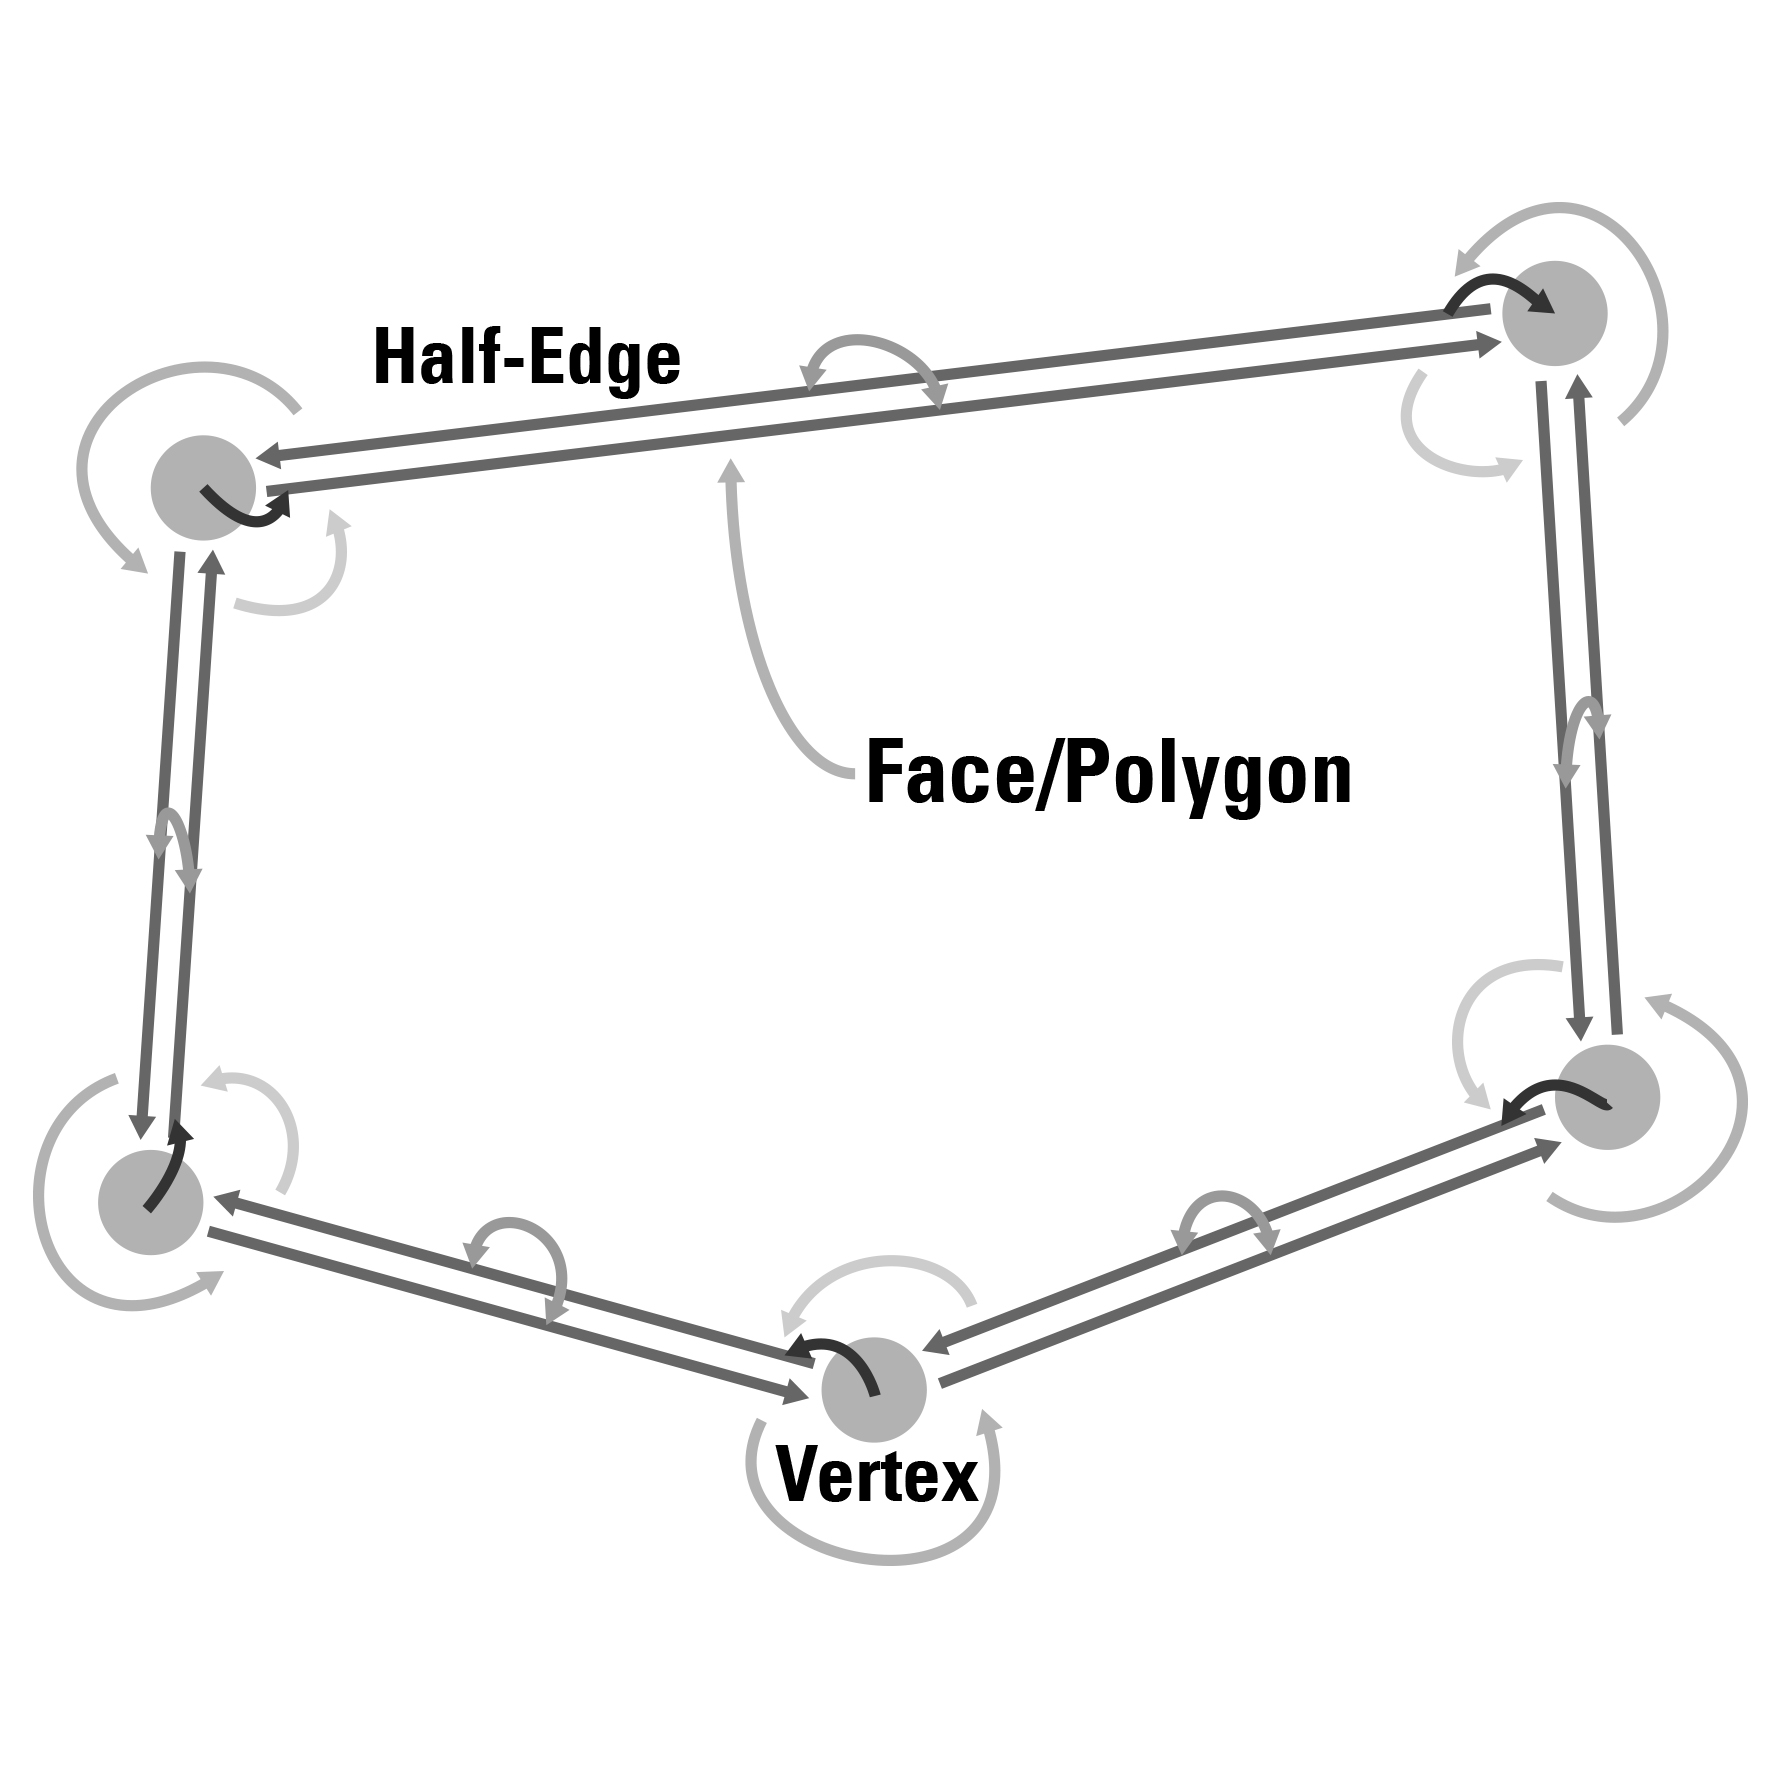
\includegraphics[width=\linewidth]{../Bilder/hesBeziehungen}
\captionof{figure}{Diese Illustration zeigt die Verbindung der data records an einem beliebigen Polygon durch Pfeilverbindungen.}\label{pic:polyConnections} 
\vspace{15mm}
An dieser Stelle sei bereits vorweg genommen, dass \LFGS in seiner Implementierung diese data records um ein paar Beziehungen, welche durch die Verbindung zur Echtzeit 3D Engine Fusee n"otig werden, erweitert.

%Content
		\subsection {Vorteile der \HES}
			%Content
			%TODO rasche geschwindigkeit in iterationen. Beispiel für einen Algorithmus anführen der Kanten eines Polygons sucht oder sonstwie über ein Polygon iteriert.
			% Exemplarisch herausfinden wie das Polygon neben einem Würfel heisst das zwischen zwei vertices liegt.
			Die vielen Verbindungen unter den einzelnen Komponenten in der \HES machen es m"oglich sehr schnelle Iterations Algorithmen zu implementieren. Die Normale\footnote{Normale: Orthogonaler Vektor auf einer Ebene. In der Computergrafik oft dazu benutzt um herauszufinden welche Seite des Faces "`vorne"' ist. Ebenfalls oft f"ur Beleuchtungsberechnung benutzt.} eines Faces kann sehr effizient berechnet werden. Es k"onnen auch die Normalen f"ur beliebige Faces unabh"angig vom Rest des Meshes berechnet werden. Man ben"otigt daf"ur lediglich den Index eines Faces als Einstiegspunkt in die Berechnung.
\newline

Subdivision Surface Algorithmen wie Catmull-Clark oder Loop k"onnen mit der Datenstruktur (oder jeder anderen Edge basierten Datenstruktur) besonders "`kosteng"unstig"' realisiert werden. Catmull-Clark ben"otigt dazu ein Mesh aus Quads w"ahrend man mit Loop ein Mesh aus Triangles verarbeiten k"onnte. Beide Mesh Typen, Quads und Triangles, werden vom \LFGS Projekt unterst"utzt. Die Fusee Engine, in welche das \LFGS Projekt integriert ist, kann im Moment allerdings nur mit Meshes bestehend aus Triangles arbeiten. Um trotzdem mit Fusee zu arbeiten, trianguliert dieses Projekt ein Mesh vor der "Ubergabe an Fusee.
\newline

Die \HES ist also grunds"atzlich sehr flexibel. Es bedingt praktisch nicht, dass die Anzahl der Eckpunkte jedes Faces eines Meshes gleich gro"s ist. \LFGS allerdings, in seiner jetzigen Form, erwartet entweder Triangulated Meshes, Meshes aus Quadlaterals (Quads) oder eine Mischung aus beidem. Dies ist dem Umstand geschuldet, dass ein Mesh zur weiteren Verwendung in Fusee konvertiert und verarbeitet werden muss.
		\subsection {Nachteile der \HES}
			%Content
Es gibt selbst in einer so flexiblen Datenstruktur wie der \HES Nachteile, die w"ahrend der Planungsphase oder Implementierung auftreten k"onnen.
			Durch ihren Aufbau und die verschiedenen Verbindung welche w"ahrend einer Initialisierung aufgebaut werden m"ussen ist die Datenstruktur sehr komplex. Es erfordert einiges an Zeit und "Uberlegungen ein System f"ur eine Implementierung so zu entwerfen, dass es alle Anforderungen an eine Echtzeit 3D Datenstruktur erf"ullt. Vor einer Implementierung der \HES sollte also gut "uberlegt sein, ob sie f"ur das gestellte Problem eine vern"unftige Art der L"osung darstellt. In \LFGS ist die Datenstruktur eine sehr elegante L"osung. Sie ist hinreichend flexibel um eine m"ogliche L"osung f"ur die Problemstellung "`(Editierbare) Echtzeit 3D Datenstruktur"' darzustellen. Die \HES ist aber nicht als Universall"osung zu betrachten. Wenn der Entwickler nur einige wenige spezielle Operationen auf einem Mesh ausf"uhren m"ochte, so gibt es m"oglicherweise eine effizientere und schnellere Datenstruktur um dies zu bewerkstelligen.

Ein auff"alliger Unterschied zu einfacheren Face basierten Datenstrukturen ist der massiv erh"ohte Overhead, der bei der Erstellung der Datenstruktur entsteht. Im n"achsten Abschnitt wird ein kleines Beispiel exemplarisch den Speicherverbrauch der \HES bestimmen.

\subsubsection {Speicherverbrauch im Gegensatz zu Face basierten Datenstrukturen}
			%Content
			Der Overhead, der bei der Repr"asentation eines Meshes f"ur eine \HES entsteht, ist um einiges h"oher als der Overhead einer Face basierten L"osung. Sollte man also nur einfache Aufgaben auf einem Mesh erledigen wollen, ist an sehr wenig Speicher gebunden, oder einige wenige Operationen nur einmal ausf"uhren wollen so w"are es wohl ratsam eine andere Datenstruktur daf"ur zu nutzen. Allerdings ist es heute in der Computergrafik meistens so, dass gen"ugend Speicherplatz im Prim"arspeicher unserer Rechner und Grafikkarten zur Verf"ugung steht um diesen Sachverhalt zu verschmerzen.
\newline

Es folgt die beispielhafte Berechnung des Speicherbedarfs eines W"urfels.
Man gehe davon aus, jedes gespeicherte Element (Daten in Form von Vertices, Faces, Edges, Half-Edges) wird mit 32bit repr"asentiert. Jeder Zeiger (Pointer) wird mit 8bit repr"asentiert. In diesem Fall k"onnte man den Speicherverbrauch zur Laufzeit des Programms im Hauptspeicher des Rechners (RAM) eines einfachen sechs Seitigen W"urfels wie folgt beschreiben.

\begin{itemize}
\item 24 Half-Edges jede beansprucht 32 bit
	\begin{enumerate}
    	\item Ein Vertex Pointer mit 8bit
    	\item Ein Twin Pointer mit 8bit
    	\item Ein Next Pointer mit 8bit
    	\item Ein Face Pointer mit 8bit
	\end{enumerate}
\item 12 Edges jede beansprucht 32 bit
	\begin{enumerate}
    	\item Zwei Half-Edge Pointer mit je 8bit
	\end{enumerate}
\item 6 Faces jedes beansprucht 32 bit
	\begin{enumerate}
    	\item Half-Edge Pointer eins mit 8bit
	\end{enumerate}
\item 8 Vertices jeder beansprucht 32 bit
	\begin{enumerate}
    	\item Half-Edge Pointer eins mit 8bit
	\end{enumerate}
\end{itemize}

Daraus w"urden sich nun folgende Berechnungen ergeben:

	Half-Edge Datenmenge: \begin{math}24 * (32bit+ 8bit + 8bit + 8bit + 8bit) = 1536bit\end{math}
	\\
	Edge Datenmenge: \begin{math}12 * (32bit + 8bit + 8bit) = 576bit\end{math}
	\\
	Face Datenmenge: \begin{math}6 * (32bit + 8bit) = 240bit\end{math}
	\\
	Vertex Datenmenge: \begin{math}8 * (32bit + 8bit) = 320bit\end{math}

	In Summe sind das 2672bit = 334 Byte.
\newline

Eine Face basierte L"osung w"urde den W"urfel so darstellen:
\begin{itemize}
\item 6 Faces jedes beansprucht 32 bit
	\begin{enumerate}
    	\item Vier Vertex Pointer mit 8bit pro Face
	\end{enumerate}
\item 8 Vertices jeder beansprucht 32 bit
\end{itemize}

Der Datenverbrauch w"urde wie folgt berechnet:

	Face Datenmenge: \begin{math}6 * (32bit + 8bit + 8bit + 8bit + 8bit) = 384bit\end{math}
	\\
	Vertex Datenmenge: \begin{math}8 * 32bit = 256bit\end{math}

	In Summe sind das 640bit = 80Byte.
\newline

Das Beispiel zeigt also, dass bei einem einfachen Mesh der Speicherverbrauch der \HES mit 334Byte um ca. das vierfache h"oher liegt als der Verbrauch einer Face basierten L"osung mit 80 Byte. Somit ist eine Face basierte Datenstruktur sparsamer was den Speicher betrifft. Allerdings tauscht man in diesem Falle auch Geschwindigkeit gegen Speicherplatz ein. Die \HES mag zwar komplex sein und hat einen h"oheren Speicherverbauch, allerdings ist sie bei Iterationen in Kantenbasierten Algorithmen auch schneller als die Face basierte Datenstruktur.
	\section {Aktueller Forschungsstatus auf dem Gebiet der 3D Mesh Datenstrukturen}
		%Content
		% TODO
		% Erwähnen und einordnen von OpenMesh, zusätzlich noch mal eben recherchieren ob es neue Implementierungen der dcel oder der hes gibt welche sich in einer 3d engine oder dergleichen bewegen.
		Die \HES oder auch die Doubly-connected edge list (DCEL) werden heute zwar relativ h"aufig f"ur 3D Mesh Datenstrukturen eingesetzt, allerdings ist zum Zeitpunkt dieser Arbeit nicht bekannt ob und welche gro"sen Programme diese Datenstruktur zum Handling ihrer 3D Daten einsetzt. Weder f"ur 3DS Max von Autodesk noch f"ur Cinema 4D von Maxon konnten verl"assliche Quellen gefunden werden. Die Open Source Software "`Blender"' verwendet in der Version 2.6 die BMesh Structure. Hierbei handelt es sich um eine vom Blender Team entwickelte Datenstruktur, welche dazu gedacht ist Limitierungen einer "alteren von Blender genutzen Datenstruktur zu beheben. BMesh\footnote{\url{http://wiki.blender.org/index.php/Dev:2.6/Source/Modeling/BMesh/Design} (gepr"uft 30.07.2013)}  ist eine an die Radial Edge Structure \footnote{Weiler, K.J. : The Radial Edge Structure: A Topological Representation for Non-Manifold Geometric Modeling. in Geometric Modeling for CAD Applications, Springer Verlag, May 1986.} angelehnte Struktur. Sie ist der \HES "ahnlich, beide weichen allerdings im Aufbau doch so stark von einander ab um sie sicher zu unterscheiden (Hier sei nur kurz angemerkt, dass BMesh nur auf komplette Kanten setzt und nicht auf Halbkanten). Wo wird die \HES also eingesetzt? Bei den Recherchen zu dieser Arbeit wurde festgestellt, dass viele Studenten und Akademiker diese Datenstruktur f"ur kleine Projekte in der Computergrafik nutzen. Es existieren einige exemplarische Implementierungen ohne die Integration in eine Engine, meistens jedoch in C++ geschrieben und dementsprechend ohne die Nutzung und Unterst"utzung von LINQ. Keines der gefundenen Projekte war in eine Echtzeit 3D Engine integriert. Es wurden auch keine geometrischen Transformationen auf den Datenstrukturen pr"asentiert. Es soll hier aber auf Ryan Holmes Arbeit \cite{Holmes.2012} verwiesen werden. Er hat ein interessantes Projekt Namens "`The DCEL Data Structure for 3D Graphics"'\footnote{Zu finden unter \url{http://www.holmes3d.net/graphics/dcel/}(gepr"uft 30.07.2013)} auf Basis der Doubly-connected edge list erstellt. Es vereinfacht den Einstieg in die Thematik und erkl"art interaktiv die Topologie der \HES und der DCEL.
\newline

Sicherlich kann diese Arbeit auch nicht fortfahren ohne die Erw"ahnung des OpenMesh\footnote{Zu finden unter \url{http://www.openmesh.org/} (gepr"uft 29.07.2013)} Projektes, betreut von Prof. Dr. Leif Kobbelt in der Computer Graphics Group der RWTH Aachen. OpenMesh ist eine generische Datenstruktur f"ur die Repr"asentation und Manipulation von polygonalen Mesh Daten \cite{Kobbelt.2013}. OpenMesh war in den Anf"angen dieser Arbeit ein Vorbild f"ur das LFG Projekt ohne jedoch den Anspruch, die Funktionen von OpenMesh nachzubilden. Open Mesh ist zudem Open Source, generisch und in C++ implementiert was einen Vergleich mit LFG zu schwierig macht. LFG orientiert sich in seiner Umsetzung jedoch ausdr"ucklich am Modell der \HES, wie sie durch M.Botsch, S.Steinberg, S.Bischoff und L.Kobbelt im Paper "`OpenMesh - a generic and efficient polygon mesh data structure"' \cite{Botsch.2002} erl"autert wird.
		%Content
		\subsection {Probleme in der aktuellen Forschung}
			%Content
			Das Problem der aktuellen Forschung ist also, dass die \HES nur sehr selten in \CSS, wenn "uberhaupt nur testweise (meist sehr minimal oder sogar nur in Pseudocode), implementiert wurde und keine der L"osungen einen Support f"ur LINQ Abfragen und Lambda Ausdr"ucke bietet. Somit ist LFG in Verbindung mit der Fusee Engine und dem LINQ Support eine neue Entwicklung auf Basis bew"ahrter Strukturen.
	\section {Einführung zu LINQ in \CS}
		%Content
		Language Integrated Query, kurz LINQ und zu deutsch Sprachintegrierte Abfrage, wurde mit \CSS 3.0 und .NET 2.0 in die .NET Umgebung integriert. LINQ ist also ein Produkt von Microsoft und erinnert auf den ersten Blick in seinem syntaktischen und semantischem Aufbau stark an die Software MySQL, eine Sprache f"ur die Verwaltung relationaler Datenbanken, welche aktuell (Stand Juli 2013) von der Oracle Corporation betreut wird. Beide Projekte unterscheiden sich jedoch wesentlich. LINQ ist in erster Linie ein Feature, das direkt auf Objekten arbeitet wohingegen MySQL auf relationale Datenbanken angewendet wird. Allerdings kann LINQ viel mehr als das. LINQ Statements werden zur "`Compile Zeit"' auf die Korrektheit der Syntax "uberpr"uft und von Microsofts IntelliSense zum Zeitpunkt der Entwicklung auf Fehler untersucht. Was einen gr"ossen Vorteil des Systems im Gegensatz zu Sprachen wie MySQL darstellt, da Statements in dieser Sprache vor Ausf"uhrung keiner syntaktischen Pr"ufung unterzogen werden.
\newline

LINQ kann als Layer und Bindeglied zwischen Collections aus Daten und den Programmiersprachen des .NET Frameworks betrachtet werden. Es ist hierbei m"oglich, LINQ in verschiedenen Bereichen zu nutzen. Es arbeitet sowohl wie bereits erw"ahnt auf Collections aus Daten, wie z.B. Listen aus Objekten die sich bereits im Hauptspeicher befinden, oder fungiert als Bindeglied zu SQL um Daten aus einem Persistenten Medium wie der Festplatte eines Rechners (Sekund"ar Speicher, HDD/SSD) auszulesen. Hierzu z"ahlen z.B. XML Datens"atzen bzw. Dokumente. Das System ist ebenso dazu in der Lage mit Filesystemen und anderen Datenquellen zu interagieren. Das bedeutet, dass LINQ sich nicht grunds"atzlich auf die vorher genannten M"oglichkeiten beschr"ankt sondern offen ist f"ur viele Arten von Datenstrukturen. Weitere Provider sind LINQ to DataSet und LINQ to SharePoint auf die hier mangels Relevanz zum Projekt nicht weiter eingegangen wird.
\newline

Noch einmal zusammengefasst zeichnen sich als wichtigste Einsatzgebiete f"ur LINQ also die folgenden Methoden aus. Im .NET Namespace finden sich die LINQ Methoden unter System.Linq
\begin{itemize}
\item LINQ to Objects ist die Basis f"ur LINQ Abfragen in .NET. Dieser Provider kann auf alle internen .NET Datenstrukturen oder Benutzerdefinierten Datenstrukturen ausgef"uhrt werden solange die Schnittstelle IEnumerable oder IEnumerable<T> f"ur generische Datenstrukturen implementiert wird.
\item LINQ to SQL ist dazu geeignet auf SQL Datenbanken, besonders auf den Versionen von Microsoft zu arbeiten.
\item LINQ to XML ist ein Provider der f"ur eine Zusammenarbeit mit XML genutzt wird. Es handelt sich hierbei um eine XML Programmierschnittstelle. \cite{MicrosoftCReferenz.2013} \footnote{\url{http://msdn.microsoft.com/de-de/library/vstudio/bb387098.aspx} (gepr"uft 01.08.2013)}
\end{itemize}

Diese Arbeit besch"aftigt sich also haupts"achlich mit dem LINQ Provider (LINQ Anbieter) LINQ to Objects, da sich die zu verarbeitenden Daten w"ahrend der Bearbeitungszeit mit LINQ bereits im Speicher des Rechners befinden. Wie erw"ahnt, ist LINQ ein Layer f"ur die Programmiersprachen von .NET und kann deswegen nicht nur in \CSS verwendet werden wie hier, sondern auch in Microsofts VB.NET. Dieses Projekt beschr"ankt sich auf \CSS als Programmiersprache, weswegen auch alle folgenden Codebeispiele in \CSS geschrieben sind. %Ein weiterer nicht zu verachtender Vorteil von LINQ im Gegensatz zu den meisten Implementationen von SQL Statements ist, dass die Statemtents vom \CSS compiler zum Zeitpunkt der Kompilierung auf syntaktische Korrektheit gepr"uft werden und der Benutzer vom IntelliSense System von Visual Studio wertvolle Hinweise w"ahrend der Generierung von LINQ Statements erh"alt.
		%Content
		\subsection {Was ist LINQ to Objects genau? }
		%Content
		LINQ to Objects wie in diesem Projekt verwendet, erfordert zur Benutzung erst einmal die grunds"atzliche Eigenschaft des Datensatzes eine Collection zu sein. Jede Collection aus Objekten, auf welche ein LINQ to objects angewendet wird, muss also die Schnittstelle IEnumerable\GTS implementieren. Diese Objekte werden im LINQ Vokabular dann als Sequences bezeichnet. In dieser Arbeit werden fast aussschliesslich die generischen Collections von \CSS verwendet welche grunds"atzlich auch alle das generische IEnumerable\GTS Interface implementieren. Der am meisten verwendete Datentyp in dieser Arbeit ist die generischen Implementierung von List\GT.

Eine LINQ to object Abfrage besteht immer aus drei Abfrageoperationen
\begin{itemize}
\item Bereitstellen einer Datenquelle
\item Erstellen einer LINQ Abfrage
\item Ausführen der LINQ Abfrage auf der Datenquelle mithilfe einer foreach() Anweisung
\end{itemize}
Das besondere an der Formulierung von LINQ Statements ist, dass sie zum Zeitpunkt ihrer Erstellung noch keine Daten der Datenquelle abfragen, sondern erst zum Ausf"uhrungszeitpunkt des Statements damit beginnen. Das ist sehr praktisch, denn dadurch k"onnen einmal in einer Abfrage erstellte Statements wiederverwertet werden. Eine LINQ Abfrage Variable speichert nie das Ergebnis einer Abfrage. Durch diesen Umstand ist es möglich, einen Datensatz zu unterschiedlichen Zeitpunkten abzufragen. Eventuell "andert sich auch das Ergebnis der Abfrage, wenn man davon ausgeht dass sich die Collection der Daten "uber die Zeit ver"andert. Trotzdem wird immer noch die semantisch gleiche Abfrage verwendet. LINQ Abfragen werden also mit einer Verz"ogerung schlussendlich in einer foreach() Anweisung ausgef"uhrt. Dabei durchl"auft die foreach() Anweisung Syntaktisch die Query oder Statement Variable und nicht die Collection der Daten.
\newline

Hier folgt ein Beispiel zu einer einfachen LINQ Abfrage auf einem einfachen Array Datensatz, welcher die Schnitstelle IEnumerable\GTS implementiert.
\lstinputlisting
			[caption={LINQeasyQuery.cs - Einfaches LINQ Abfrage Beispiel}, label=code:linqeasyquery]
			{../Codebeispiele/LINQeasyQuery.cs}

Ein direkter Aufruf der Methoden toList\GTS oder toArray\GTS auf dem Statement erzwingt die sofortige Ausf"uhrung der Abfrage.
%\caption[Foo Bar.]{Foo Bar. Redrawn from \protect\cite{Baz}.}
\lstinputlisting
			[caption={LINQdirectQueryList.cs - Einfaches direktes LINQ Abfrage Beispiel} \protect\cite{MicrosoftCReferenz.2013}, label=code:linqdirectquery]
			{../Codebeispiele/LINQdirectQueryList.cs}
		%Content
		\subsection {Abfragesyntax in LINQ}
		Was im vorigen Code Beispiel \ref{code:linqdirectquery} als LINQ Statement bezeichnet wurde ist eigentlich ein ganz spezielles LINQ Statemtent in einer speziellen syntaktischen Schreibweise. In diesem Fall ein LINQ Statement geschrieben in der Abfragesyntax. Diese Syntax zeichnet sich durch einfache Lesbarkeit und einfache Zug"anglichkeit aus. Zur Compile Zeit wird diese Syntax vom Compiler in die so genannte Methodensyntax "ubersetzt. Die beiden syntaktischen Varianten sind semantisch identisch auch wenn sie sich auf den ersten Blick sehr unterscheiden.
		%Content
		\subsection {Methodensyntax in LINQ}
		Die Methodensyntax in LINQ unterscheidet sich von der Abfragesyntax dadurch, dass anstatt fester Keywords wie where, from und select um eine Abfrage zu formen, Lambda Ausdr"ucke verwendet werden (Lambda Ausdr"ucke werden im n"achsten Abschnitt n"aher erleutert). In der Referenzdokumentation zu LINQ (Stand Juli 2013) \cite{MicrosoftCReferenz.2013} wird haupts"achlich diese Art der Syntax verwendet. Aus den dort aufgef"uhrten Typen wird in dieser Arbeit sehr h"aufig der Enumerable Typ verwendet.
\\
Hier ein Vergleich der beiden Syntaktischen M"oglichkeiten zum Erstellen von LINQ Statements.
\lstinputlisting
			[caption={LINQzweiSynt.cs - Zwei syntaktische M"oglichkeiten} \protect\cite{MicrosoftCReferenz.2013}, label=code:linqzweisynt]
			{../Codebeispiele/LINQzweiSynt.cs}
		%Content

Beide Methoden LINQ Abfragen in \CSS zu schreiben werden vom JIT (Just in Time Compiler) in gleichen Code "ubersetzt. Sie unterscheiden sich nur selten. Manche Standardoperatoren wie Sum oder Count sind in der Abfragesyntax nicht gegeben. Dieses Projekt wird in Zukunft alle LINQ Abfragen in der Methodensyntax verwenden um den Code zu vereinheitlichen. Der Entwickler kann sich also eigentlich aussuchen, in welcher Syntax er seinen Code am liebsten schreibt. Eine gute "ubersicht von LINQ Standard Operatoren wurde von Don Box und Anders Hejlsberg 2007 in \begin{quote}"`LINQ: .NET Language-Integrated Query"' \cite[Standard Query Operators in a Nutshell]{Box.2007}\end{quote} beschrieben. \footnote{Zu finden unter \url{http://msdn.microsoft.com/en-us/library/bb308959.aspx}}
\newpage
Hier sollen nur die f"ur dieses Projekt wichtigsten Standardoperatoren aufgelistet werden.
\newline

\addcontentsline{lot}{table}{Standardoperatoren in LINQ}\label{tab:standardoperatoren}
\begin{tabular}{p{3cm}|p{9cm} |l|l|}
\hline
  Operator & Beschreibung\\
\hline
\hline
  Select & Ein Projektionsoperator der auf einer Auswahlfunktion basiert.\\
\hline
  Where & Ein Restriktionsparemeter, seine Entscheidungen basieren auf einem angegebenen
 Pr"adikatausdruck\\
\hline
AsEnumerable & Konvertiert eine Collection in ein Objekt vom generischen Typ IEnumerable<T>\\
\hline
ToArray, ToList & Konvertiert eine Collection in ein Array oder eine Liste\\
\hline
Contains & Pr"uft ob ein Element in der Collection vorhanden ist\\
\hline
Distinct & Entfernt Duplikate aus einer Collection \\
\hline
\end{tabular}

\newpage
	\section {Einführung zu Lambda Ausdr"ucken in \CS}
		%Content
		Lambda Ausdr"ucke in \CSS sind Anonymen Funktionen sehr "ahnlich. In dieser Arbeit wurden Lambda Ausdr"ucke in LINQ Statements im Zusammenhang mit Standardabfrageoperatoren verwendet. Syntaktisch ist diese Art Funktionen zu schreiben sehr simpel gestrickt. Das Lambda Zeichen in \CSS wird als \LAM dargestellt. Es folgt immer der Parameterliste und sollte nicht mit den Vergleichsoperatoren \textgreater = und \textless = verwechselt werden. Das Lamba Zeichen bedeutet hier soviel wie "`wechselt zu"' oder "`wird zu"' und steht links des gew"unschten Ausdrucks.
		%Content
		\subsection {Lambda Ausdr"ucke in Verbindung mit LINQ}
Wie bereits beschrieben werden Lambda Ausdr"ucke  in Verbindung mit LINQ in der Methodensyntax von LINQ verwendet. Diese Syntax wird meist benutzt um Standardabfrageoperatoren wie Collection.Select(lambda hier) Collection.Where(lambda hier) und Collection.All(lambda hier) zu verwenden. In dieser Arbeit wird der Standardoperator Select() am h"aufigsten verwendet. Select() wendet den angegebenen Lambda Ausdruck auf jedes Element der Collection an auf die der Select operator angewendet wird und gibt, falls vorhanden, ein Ergebnis zur"uck. Siehe Listing \ref{code:lambdaeasy}

Lambda ist also eine einfache M"oglichkeit Standard LINQ Abfragen aufzuwerten. Es reicht im Hinblick auf dieses Projekt meist zur Abfrage von Informationen aus. Oft kommt es vor, dass mehrere LINQ Abfragen mit Lambda Statements kombiniert werden um ein Ergebnisset zu erhalten. 
\lstinputlisting
			[caption={LambdaEasy.cs - Einfacher Lambda Ausdruck}, label=code:lambdaeasy]
			{../Codebeispiele/LambdaEasy.cs}


\section {Das Software Projekt LINQ For Geometry}
		%Content
Das Softwareprojekt \LFGS (kurz LFG), welches im Rahmen dieser Thesis Arbeit entworfen und implementiert wurde, stellt eine Umsetzung der \HES zum Handling dreidimensionaler Meshes dar. \LFGS hat darüber hinaus den Anspruch, die Datenstruktur durch LINQ Ausdr"ucke und bereit gestellte Iteratoren/Enumeratoren, welche mit LINQ erweitert werden k"onnen, flexibel und zug"anglich zu gestalten. Es bietet einen Converter in das von der Fusee Engine benutze Mesh Format und kann in Echtzeit geometrische Operationen auf einem in der Datenstruktur gespeichertem Mesh ausf"uhren. \LFGS wurde Anfangs als eigenst"andiges Projekt begonnen. Im sp"ateren Verlauf wurde es in die Fusee Engine integriert um dort wahlweise Meshes in der \HES im Speicher bereit zu halten. Das \LFGS Projekt ist von Fusee nicht abh"angig. es w"are also nach Wunsch auf andere Engines oder Programme mit wenigen Anpassungen portabel.

\LFGS erweitert die \HES um ein paar Funktionen um die korrekte Darstellung von Meshes in Fusee zu gew"ahrleisten. Dazu z"ahlen Erweiterungen der an den Kanten und Faces gespeicherten Informationen, um UV Textur Koordinaten und Face- und Vertex Normalen im Mesh zu speichern.
Zus"atzlich ist es in der Lage, Kanten zu verarbeiten, die an mehr als 2 Polygone grenzen. Diese L"osung ist allerdings zum Zeitpunkt Juni 2013 nur als Notl"osung zu betrachten und das massive Edge Sharing (Teilen von Kanten mit vielen Faces) sollte wenn m"oglich bereits beim Modellieren eines Meshes vermieden werden.
\newline

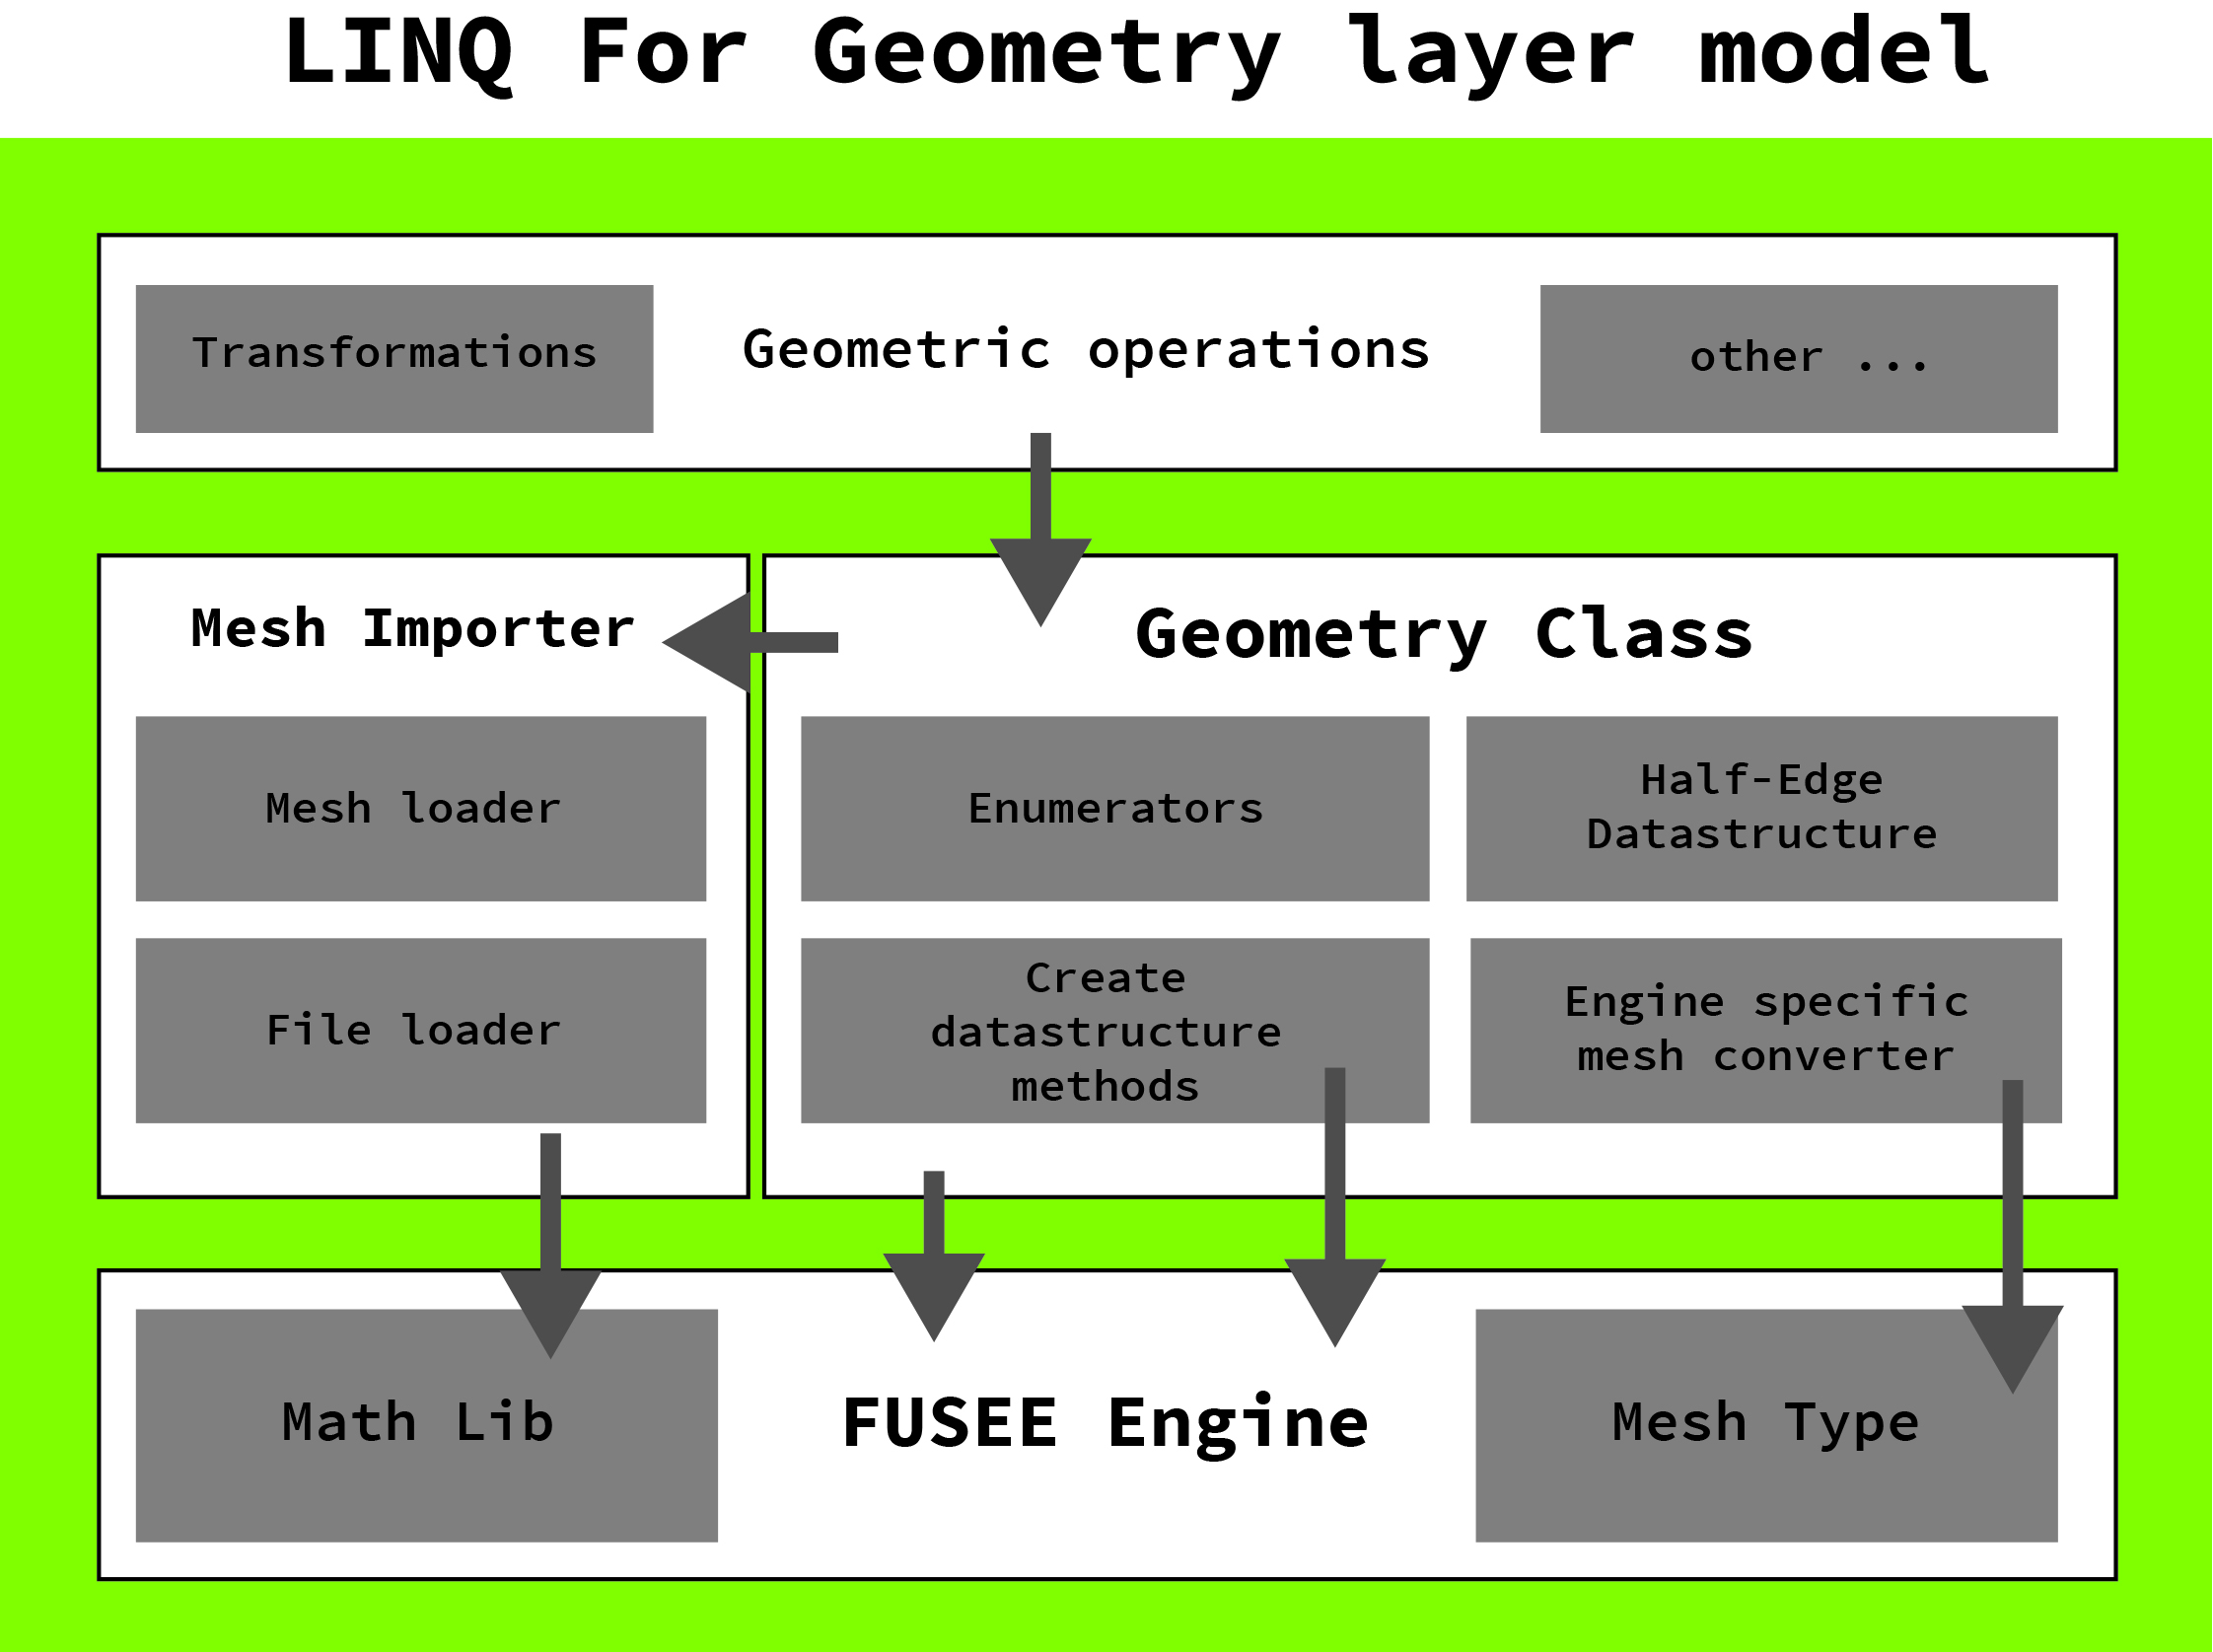
\includegraphics[width=\linewidth]{../Bilder/LFGLayer}
\captionof{figure}{Diese Illustration zeigt die verschiedenen Layer von LFG und deren Verbindungen.}\label{pic:LFGLayer} 


In den n"achsten Abschnitten steht die Implementierung, siehe \ref{uml:klassendiagramm}, von \LFGS im Vordergrund und versucht ein Umfassendes Bild zu vermitteln wie die \HES mit Hilfe von LINQ und Lambda Support in \CSS aufgebaut werden kann.
\newline
		%Content
		\subsection {Konzept zu \LFG}
			%Content
			% Was ist das Konzept von LFG, wann hat es sich in Fusee integriert. Wieso ist es so wichtig die hes einzusetzen.
			% TODO Klassen Diagramme und UML etc.
			Das \LFGS Projekt begann als Thesis Projekt, in welchem angedacht war die \HES in \CSS zu implementieren und ihre M"oglichkeiten in Verbindung mit LINQ ausfindig zu machen. Nach einer Weile zeigte sich jedoch, dass es wesentlich interessanter w"are, dieses Projekt in einer echten 3D Echtzeit Engine einzusetzten und die M"oglichkeiten direkt in der Engine auszuwerten. Das Projekt wurde dann im n"achsten Schritt in einem extra Branch in die Fusee Engine intergiert. Der Branch in welchem sich \LFGS aktuell (25. Juli 2013) befindet ist stehts auf dem aktuellen Stand des Fusee development Branches (develop). Alle Ver"anderungen des Fusee Projekts wurden w"ahrend dieser Arbeit sofort eingepflegt um m"oglichen sp"ateren Problemen entgegen zu wirken. Diese Arbeit ist von Fusee trotz der engen Bindung als Geometry Datenstruktur fast nahtlos abgekoppelt. Die einzigen Referenzen welche \LFGS auf Fusee enth"alt beziehen sich auf die Mathematik Bibliothek von Fusee und das von Fusee genutze Mesh Format. \LFGS kann dadurch recht einfach von Fusee gel"ost und in eine andere Engine integriert werden. Lediglich die toMesh() Methode von LFG m"usste dann auf eine neue Engine angepasst werden, falls sich deren Mesh Repr"asentation von der bereits in Fusee implementierten Variante unterscheidet.
%TODO Grafik vom Klassendiagramm und vom External Module
%TODO Erklärung warum LFG so offen ist. Performance, Einfachheit, Ziel der Arbeit ist eine schnelle Schnittstelle die einfach für jeden benutzbar ist.
\newline

\LFGS stellt wie alle interessanten Anwendungsm"oglichkeiten in Fusee ein eigenes Beispiel Projekt im Projektmappenordner "`Examples"' bereit. In diesem Beispiel dreht sich alles um die Verwendung von LFG als Handler f"ur die Mesh Daten und dessen M"oglichkeiten. Verschiedene Modelle k"onnen als Mesh in eine Fusee Applikation geladen werden und durch verschiedene Tastenbelegungen welche in der Methode  PullUserInput() hinterlegt sind auch transformiert werden. Aktuell bietet das Beispiel Projekt an, ein Mesh Objekt zu skalieren, es zu drehen, es zu verschieben und die Berechnung der Vertex Normalen aus zu schalten. Alle Berechnungen f"ur die Transformationen laufen dabei direkt auf der \HES in \LFGS ab und werden nicht durch die Fusee Engine beeinflusst. F"ur die sp"ater noch angesprochenen Benchmarks, verf"ugt das Projekt "uber eine Demo Funktion welche das Mesh in vorher festgelegten Zeitabst"anden durch die bereitgestellten Transformationen bearbeitet. Durch den frei konfigurierbaren Ablauf und die Settings der Demo biett sie eine gute Basis f"ur Benchmarks.
% TODO UML Ablaufdiagramm hier
\newline

In Zukunft ist es angedacht, das Projekt \LFGS m"oglicherweise als eine 3D Editor Datenstruktur in Fusee zu verwenden. Es ist ebenfalls denkbar, das Projekt einzusetzen wenn sich Meshes in einer Applikation zur Laufzeit dynamisch ver"andern sollen. Durch die massive Vernetzung der einzelnen Elemente (Half-Edges, Vertices, Faces) der \HES ist das Projekt sehr flexibel einsetzbar. Das VisualStudio Projekt "`LingForGeometry.ExternalModules"' welches mit dem \LFGS Branch von Fusee mitgeliefert wird, ist ein Projekt um die Funktionen dieser Arbeit zu erweitern ohne den Core Code ver"andern zu m"ussen. Das Projekt hat Zugriff auf alle wichtigen Iteratoren/Enumeratoren (LINQ und nicht LINQ basiert) und Collections aus Daten. Um ein Beispiel f"ur diese Funktionen zu haben wurden alle Geometrischen Operationen und Transformationen als externe Funktionen im ExternalModules Projekt implementiert.
			%Content
		\subsection {Furtwangen University Simulation and Entertainment Engine}\label{sec:fusee}
			%Content
			Die Furtwangen University Simulation and Entertainment Engine (kurz Fusee) ist eine Open Source 3D Echtzeit Engine mit einem Schwerpunkt auf einer Multiplattform Unterstützung. Entwickelt wurde sie von einer Projektgruppe an der Hochschule Furtwangen unter der Leitung von Herrn Prof. M"uller an der Fakult"at Digitale Medien.Von der aktuellen Version 0.5 werden folgende Plattformen unterst"utzt.
\begin{itemize}
\item Windows OS
\item Linux OS
\item Android OS
\item Die Android Konsole OUYA
\item Der Chrome Browser
\item Der Firefox Browser
\end{itemize}

Um eine Linux und Android Unterst"utzung zu erreichen ist das Projekt mit Mono, einer .NET Open Source Implementierung, kompatibel. Sogar einen Export nach JavaScript durch den JSIL Compiler von Kevin Gadd ist m"oglich. Somit ist Fusee ohne weitere Plugins im Browser lauff"ahig.
\newpage
Hier eine Liste der bereits umgesetzten Features in der Version 0.5:
\begin{itemize}
\item Multitexturing
\item Ein standard Set an Shadern ist verf"ugbar
\item Benutzerdefinierte Shader sind m"oglich
\item Ein Scene Management wird unterst"utzt
\item Sound in Browsern und Betriebssystemen vorhanden
\end{itemize}

\LFGS ist als Projekt in einen eigenen Fusee Branch integiert. Nach aktuellem Stand (Juli 2013) kann man sich als Benutzer entscheiden, ob man dann ein Modell mit dem in Fusee integrierten Mesh System oder mit dem \HES Geometry System von \LFGS laden m"ochte.

Als Schnittstelle zur GPU (Graphics Processing Unit) verwendet Fusee die low level Bibliothek OpenTK\footnote{\url{http://www.opentk.com/ (gepr"uft 30.07.2013)}} welche in \CSS geschrieben ist und einen wrapper f"ur die OpenGL Multi platform application programming interface (API) darstellt.

Weitere Informationen "uber die Fusee Engine sind auf der offiziellen Homepage\footnote{\url{http://fusee3d.org/}} oder "uber GitHub\footnote{\url{https://github.com/FUSEEProjectTeam/Fusee}} erh"ltlich.\footnote{Quelle \url{http://fusee3d.org/about/} (Stand 19.07.2013)}
			%Content
\section {Die Vorteile in der Entwicklung mit managed Programmiersprachen}\label{sec:VorteileManaged}
		%Content
Durch die enge Verkn"upfung von \LFGS mit der Fusee Engine war es sinnvoll, das Projekt in der gleichen Programmiersprache wie Fusee zu implementieren, um eine Kommunikation der beiden Projekte m"oglichst einfach zu gestalten. Obwohl die .NET Basis hier nat"urlich Spielraum f"ur Entscheidungen zugunsten VB.NET gelassen h"atte. Sinnvoll w"are das nat"urlich nicht gewesen. Hier soll jetzt kurz gekl"art werden was "`Managed Code"' genau bietet und warum \LFGS in einer solchen Sprache wie \CSS implementiert wurde. Nat"urlich einmal davon abgesehen, dass \LFGS mithilfe von LINQ implementiert wurde und LINQ eine der S"aulen des Projekts darstellt.

		Managed Code bietet einem Entwickler viele verschiedene Vorteile im Gegensatz zur Entwicklung in einer Nativen Programmiersprache. Im Hinblick auf die \HES sollte besonders das Speichermanagement und die Pointer Verwaltung betrachtet werden. Durch die in \CSS implementierte Garbage Collection ist der Programmierer von der Aufgabe befreit, das Speichermanagement selbst zu verwalten. Das bietet einen gro"sen Vorteil in der schnellen Entwicklung von Programmiersprachen. Managed Code ist f"ur viele Entwickler einfacher zu schreiben als native Code in Sprachen wie z.B. C++.

Im Hinblick auf \LFGS f"allt durch die Nutzung von \CSS einiges an Arbeit weg. Nicht mehr gebrauchte tempor"are Listen, von denen es einige im Projekt gibt und Objekte werden automatisch durch die Garbage Collection aufger"aumt und es kommt sehr selten bis kaum zu Memory Leaks durch Programmier- oder Laufzeitfehler. Es ist so wesentlich einfacher externen Nutzern einen Zugang auf den Code des Projekts zu erm"oglichen ohne dass sie Gefahr laufen, die Integrit"at der Datenstruktur durch Pointer Manipulationen zu gef"ahrden. \CSS bietet hier also ein gewisses Ma"s an Sicherheit f"ur das System.

Ein weiterer Pluspunkt ist nat"urlich, dass sich bereits viele Entwickler und Studenten der Hochschule Furtwangen, die sp"ater m"oglicherweise die Fusee Engine verwenden m"ochten, bereits mit \CSS oder Java, welches \CSS zumindest syntaktisch sehr "ahnelt, auskennen.
		%Content
		\subsection {Warum die Programmiersprache \CSS f"ur \LFG?}
			%Content
			Wie bereits im oberen Abschnitt \ref{sec:fusee} angeschnitten, wurde \LFGS f"ur eine Zusammenarbeit mit der Fusee Engine konzipiert. \LFGS bietet hierbei eine neue Geometry Objekt Klasse f"ur die Fusee Engine an, ohne die tats"achliche Klasse zu "uberschreiben. Laut aktuellem Stand kann der Benutzer beider Projekte sich also entscheiden, welche Meshes er gerne in der \HES laden m"ochte und f"ur welche es gen"ugt, sie als Face basiertes Mesh im Speicher zu halten. Diese Entscheidung l"asst dynamische Entscheidungen zu. Es ist somit im Bereich des M"oglichen, manche Meshes als unver"anderbares Fusee.Mesh zu behandeln und andere w"ahrend der Laufzeit durch LFG zu manipulieren.
\newline

Damit \LFGS auf diese Art mit der Fusee Engine kommunizieren kann, musste eine gemeinsame Schnittstelle evaluiert werden. Weil beide Projekte die .NET Plattform benutzen und Fusee in \CSS geschrieben wurde war es naheliegend f"ur \LFGS auch \CSS zu benutzen. Da der LINQ Layer ein Produkt von .NET ist, war \CSS die wohl beste Wahl um beide Projekte zusammen zu bringen.
			%Content
\subsection {Der Link von LINQ zur \HES}
				%Content
				% Wie spielt linq in lfg mit, was stützt es, wo wird es nicht verwendet, warum eigtl linq und wie arbeitet es auf den collections von lfg
				\LFGS ist durch die Bereitstellung einiger grundlegender Enumeratoren einfach zu erweitern. Um den Einsatz des Projekts f"ur externe Benutzer weiter zu vereinfachen, wurde das Hauptaugenmerk darauf gelegt, LINQ f"ur Datenabfragen auf der fertigen \HES zu verwenden. LINQ ist einfach verst"andlich und kann durch wenige Zeilen Code aufwendige traversierungs Algorithmen realisieren. Die bereits angebotenen Enumeratoren sollen im zuk"unftigen Einsatz von LFG unbedingt wiederverwendet werden und sind teilweise schon selbst nur durch Kombinationen aus anderen in LFG implementierten LINQ Abfragen aufgebaut. So ist es ein Ziel dieser Arbeit LINQ als Bindegleid und "`Schnittstelle"' zum Projekt einzusetzen und damit die Produktivit"at beim Formulieren neuer Algorithmen und Funktionen zu steigern.
				%Content
	\section {Der Import von Geometriedaten im „Wavefront Object“ Format}
		%Content
		Das Projekt \LFGS benutzt das von Wavefront Technologies entwickelte offene "`Wavefront Object"' Format (Dateiendung .obj) um Modelle aus 3D Modellierungssoftware zu importieren. Wavefront Technologies existiert heute nicht l"anger. Die Firma wurde im Jahr 1995 von Silicon Graphics augekauft und mit Alias Research zu Alias|Wavefront verschmolzen. Mittlerweile geh"oren beide Firmen zu Autodesk (3DS Max, AutoCAD).

Das .obj Format zeichnet sich durch seine einfache Form und durch die von Menschen lesbare Kodierung in ASCII aus. Bei diesem Format handelt es sich um ein Face basiertes Format zur Speicherung von Mesh Daten. Alle Vertices eines Meshes werden gespeichert und Faces definieren ihre Eckpunkte aus den Indizes der Vertices. Es ist ebenfalls m"oglich, Texturkoordinaten und Normalen zu speichern. Die optionalen Tags "`mtllib"' und "`mtl"' geben an ob Material Dateien vorliegen und wann und wo diese verwendet werden sollen. Diese Funktion wird in LFG und Fusee zum Zeitpunkt dieser Arbeit nicht unterst"utzt. Texturen werden aktuell noch als .jpg Dateien geladen. Kommentarzeilen werden mit einer Raute "`\#"' gekennzeichnet, Objekte und Gruppen von Objekten mit einem "`o"' und "`g"'. Das Wavefront .obj Format ist heute eine Art Standard. Die meisten 3D Programme k"onnen es importieren und exportieren. Dazu z"ahlen das w"ahrend dieser Arbeit verwendete Cinema 4D von Maxon, sowie die Open Source Software Blender und die Fusee Engine.
		%Content
		\subsection {Warum das Wavefront Object Format}
			%Content
			Warum verwendet LFG das Wavefront .obj Format? Einer der Wichtigsten Gr"unde ist sicherlich, dass Fusee in seiner Standard Implementierung ebenfalls dieses Format verwendet. Um die "Ubersichtlichkeit des Projektes zu erhalten und den Prozess des Imports nicht zu verkomplizieren wurde w"ahrend dieser Arbeit ebenfalls entschieden, den Import der Daten im .obj Format vorzunehmen. Der Importer von \LFGS ist jedoch ein Anderer als der Importer von Fusee. Haupts"achlich aufgrund einer fehlenden Schnittstelle und anderer Import Algorithmen. Das hat den Vorteil, dass ein sp"aterer Benutzer des Systems den Importer erweitern kann, ohne den Engine Code oder den Code von \LFGS "andern zu m"ussen. Der Importer ist vom LFG Projekt abgekoppelt. Ein Nutzer k"onnte also sogar seinen eigenen Importer f"ur ein anderes Format verwenden, solange er der Geometry Klasse das korrekte Datenformat inklusive der ben"otigten Datentypen zum Aufbau der Datenstruktur "ubergibt. Im LFG erwartet die Geometry Klasse vom Importer die "Ubergabe eine Collection (einfach verkettete Liste, in \CSS List<T>) aus "`GeoFaces"'.
\lstinputlisting
			[caption={GeoFace.cs - Ein tempor"arer Face basierter Datentyp.}, label=code:geoface, firstline=20, lastline=24]
			{../../HFU_Fusee/Fusee/src/Engine/LinqForGeometry/LinqForGeometry.Core/src/Importer/GeoFace.cs}

Ein "`GeoFace"' ist ein Konstrukt, das ein Polygon (In LFG Face genannt) eines 3D Models (Meshes) repr"asentiert. Jedes GeoFace selbst enth"alt eine Liste aus Fusee.Math float3 Vertice Daten und Fusee.Math float2 UV Koordinaten.
\newline

Im Beispiel \ref{obj:bsp} handelt es sich um einen W"urfel, der ohne Normalen oder UV Textur Koordinaten gespeichert wurde. Der W"urfel wurde aus der Software Cinema4D exportiert. Der W"urfel besteht aus Quads. Das ist daran zu erkennen, dass jedes Face 4 Vertices referenziert.
\begin{lstlisting}
# WaveFront *.obj file (generated by CINEMA 4D)

g Cube
usemtl Mat
v -100 -100 100
v -100 100 100
v 100 -100 100
v 100 100 100
v 100 -100 -100
v 100 100 -100
v -100 -100 -100
v -100 100 -100

f 3 4 2 1 
f 5 6 4 3 
f 7 8 6 5 
f 1 2 8 7 
f 4 6 8 2 
f 5 3 1 7 
\end{lstlisting}\label{obj:bsp}

			%Content
		\subsection {Der Importer für das Wavefront Format oder auch Face basierter Import - Edge basiertes Handling}
			%Content
			Zum Import Zeitpunkt eines Assets (Meshes) wird zuerst der Inhalt der im Speicher des Betriebssystems abgelegten .obj Datei komplett eingelesen. Die Datei Endung f"ur eine Mesh Datei im Fusee Universum unterscheidet sich durch die zus"atzliche Endung .model leicht von der Standard Datei Endung. So wird ein Konflikt mit den in Visual Studio benutzen Compilern und dem .obj Format f"ur kompilierte aber noch nicht gelinkte Dateien vermieden. Eine Datei w"urde dann f"ur die Verwendung in Fusee und LFG als Cube.obj.model benannt werden. Der Importer parsed jetzt alle n"otigen Strings in Integer Werte und baut aus den Face Definitionen im .obj Format "`GeoFace"' Objekte zusammen. Zu diesem Zeitpunkt liegt das komplette Mesh noch Face basiert vor. Es gibt noch keine Beziehungen zwischen den einzelnen Elementen und jedes Face steht f"ur sich alleine. Die ganze Collection an Daten wird nun von der Geometry abgeholt und durch den Initialisierungslauf in die \HES "ubersetzt. Erst entsteht aus dem Face basierten Meshe die Edge basierte Datenstruktur.
			%Content
	\section {Initialisierungsablauf und Aufbau der \HES in \LFG}
			%Content

			In diesem Abschnitt wird kurz aufgezeigt wie aus einem Face Basierten Mesh aus GeoFaces die \HES entsteht.

Die Geometry Klasse in \LFGS "ubernimmt die Speicherung der Datenstruktur ebenso wie die Umsetzung eines Meshes in diese. Ein Asset (Mesh) muss mit der Methode LoadAsset(String path) geladen werden. Die Load Asset Methode "ubernimmt den kompletten Konvertierungsprozess in die \HES. Eine Liste aus GeoFaces wird durch den Importer geladen und dieser Methode anschliessend zur Verf"ugung gestellt. Weiterhin wird nun f"ur jedes Face in der bekannten Liste durch die Methode AddFace(GeoFace face) ein Face in der Datenstruktur eingef"ugt. Der genaue Ablauf hierzu wird in UML Diagrammen dargestellt.

LINQ wird im Initialisierungslauf daf"ur eingesetzt, zu "uberpr"ufen, ob ein Vertice schon durch das Einf"ugen eines Faces in der Datenstruktur vorhanden ist, oder ob der Vertex noch eingef"ugt werden muss. Durch diese Abfrage wird verhindert, dass sich redundante Datens"atze bilden. Eine "ahnliche aber weitaus komplexere LINQ Abfrage erfolgt beim Einf"ugen der Kanten. Auch hier wird auf bereits bestehende Kanten gepr"uft. Das ist immer dann der Fall, wenn zwei Faces sich zwei Vertices teilen und das zweite Face nach dem ersten in die Datenstruktur eingef"ugt werden soll. Das System erkennt hier eine bereits bestehende Kante und anstatt eine neue Kante zu erstellen wird nur die freie Half-Edge der Kante verwendet.
\newline

Hier exemplarisch der verkettete LINQ Query zum "Uberpr"ufen der vorhandenen Kanten. Er funktioniert in diesem Fall "ahnlich einer if Abfrage und sucht per FindIndex() den Index des ersten ,Elements welches auf das angegebene Pr"adikat passt. Sollte kein passendes Element gefunden werden, so wird -1 zur"uck gegeben.

\begin{lstlisting}
_LedgePtrCont.FindIndex(
                    edgePtrCont => _LhedgePtrCont[edgePtrCont._he1]._v == fromVert && _LhedgePtrCont[edgePtrCont._he2]._v == toVert || _LhedgePtrCont[edgePtrCont._he1]._v == toVert && _LhedgePtrCont[edgePtrCont._he2]._v == fromVert)
                );
\end{lstlisting}

An dieser Stelle im Code wurde f"ur LFG eine kleine Erweiterung implementiert. Sollte eine Kante bereits von zwei Faces belegt worden sein, jedoch eine dritte Kante ebenfalls eine Kante zwischen den zwei bereits belegten Vertices fordern, so wird eine neue Kante f"ur das dritte Face eingerichtet. Dieser Vorgang ist nicht begrenzt. Der 3D Artist sollte jedoch darauf achten, dass keine Kanten im Mesh von mehr als 2 Faces benutzt werden. Dieses Fallback wurde eingebaut um, einen Crash der App im Falle eines Imports eines fehlerhaften Meshes abzufangen. Die Datenstruktur ist auf eine solche Handhabung in LFG eigentlich nicht ausgelegt.

In der AddFace() Methode werden ebenfalls die ben"otigten UV Koordinaten an den Half-Edges gespeichert. Sie werden an den Half-Edges gespeichert welche mit ihrem Vertice Handle auf die korrekten Vertices zeigen. Zuletzt werden alle Half-Edges des Faces noch miteinander verbunden. Diese Operation wird zuletzt ausgef"uhrt, weil der Index für das Handle einer Half-Edge nicht im Vorfeld berechnet werden kann. So k"onnen in einem Modell das Face Nr 1 und das Face Nr XXX nebeneinander liegen und sich m"oglicherweise manche Kanten teilen.

Ein Face muss jetzt nur noch als Face Pointer Container in das System eingef"ugt werden und LFG beginnt mit dem n"achsten Face von vorne bis alle Faces abgearbeitet wurden.

			%TODO Grafik erstellen?
			%TODO Grafik erstellen?
			%TODO Grafik erstellen?
			%Content

				%Content
	\section {Implementierung und Funktion der Handler für die einzelnen Komponenten der HES}
		%Content
Die Handler Konstrukte "`Structs"' in dieser Arbeit, welchen Datentyps auch immer, können als Zeiger auf Datens"atze von realen Daten betrachtet werden. Sie dienen als Indizes um Daten zu vernetzen und bieten eine Kontrollmethode, um zu "Uberpr"urfen ob ein Handler "`valid"' (Zul"assig, In Ordnung) ist. Ein Handler auf einen Satz von Daten kann wenn gew"unscht mehrmals verwendet werden. Dies w"urde bei geeigneter Implementierung die Menge der zu speichernden Daten um den Faktor \(n\) (\(n\) = wiederholte Nutzung des Handlers) reduzieren.
		%Content
		\subsection {Beispiel eines Handler Konstruktes und seiner Implementierung}
		%Content
Sie enthalten nur einen Index als Zeiger und sehr wenige Funktionen. Ein Handler speichert zur Laufzeit pro Instanz einen Index auf den realen Datensatz f"ur den er einen Handle darstellt. Handler Structs gibt es f"ur Edges, Half-Edges, Faces, FaceNormals, Vertices, VertexNormals und VertexUVs. Sie unterscheiden sich hierbei nur durch die Namensgebung der Structs und der Konstrukturen.
\lstinputlisting
			[caption={HandleHalf-Edge.cs - Variablen Deklaration des "`Zeigers"'}, label=code:hhezeiger, firstline=21, lastline=21]
			{../../HFU_Fusee/Fusee/src/Engine/LinqForGeometry/LinqForGeometry.Core/src/Handles/HandleHalfEdge.cs}

Ein Handler Struct stellt eine implizite Konvertierung des Handlers, siehe Listing \ref{code:hhecast}, in den Datentypen Integer (int) zur Verfügung.
\lstinputlisting
			[caption={HandleHalf-Edge.cs - Impliziter cast nach Integer}, label=code:hhecast, firstline=37, lastline=40]
			{../../HFU_Fusee/Fusee/src/Engine/LinqForGeometry/LinqForGeometry.Core/src/Handles/HandleHalfEdge.cs}

Zus"atzlich kann der Entwickler jederzeit abfragen, ob der aktuell verwendete Handler schon als valide betrachtet werden kann. Hierzu Listing \ref{code:isvalid} betrachten. Ein Handler ist dann valide, wenn sein Index nicht kleiner als 0 ist. In dieser Arbeit werden einstweilen Handler initialisiert, f"ur die zum Zeitpunkt der Initialisierung noch kein Index zur Speicherung bereit steht. Diese vorerst nicht validen Handler werden dann mit dem Wert -1 initialisiert und sind somit zu diesem Zeitpunkt als nicht valide also nicht verwendbar zu betrachten. Um diese sp"ater im Programm zu benutzen, muss also noch der korrekte Index, meistens der Wert einer Count Funktion auf einer Liste eingef"ugt werden.
\lstinputlisting
			[caption={HandleHalf-Edge.cs - Is Valid?}, label=code:isvalid, firstline=45, lastline=48]
			{../../HFU_Fusee/Fusee/src/Engine/LinqForGeometry/LinqForGeometry.Core/src/Handles/HandleHalfEdge.cs}

Eine Besonderheit der Handler ist die mit "`internal"' gekennzeichnete Deklaration der Indizes. Siehe hierzu Listing \ref{code:hheinternal}. Durch das "`internal"' \CSS Schl"usselwort k"onnen die Handler nur aus der jeweiligen gleichen Assembly angesprochen und ver"andert werden. Dies verhindert einen unbefugten oder unabsichtlichen Fremdzugriff von Au"sen. W"ahrend der Laufzeit wird also die Konsistenz der Datenstruktur in sich gesch"utzt, um so das Programm vor Abst"urzen durch Zeiger Fehler zu sch"utzen.
\lstinputlisting
			[caption={HandleHalf-Edge.cs - Deklarationen als internal}, label=code:hheinternal, firstline=21, lastline=21]
			{../../HFU_Fusee/Fusee/src/Engine/LinqForGeometry/LinqForGeometry.Core/src/Handles/HandleHalfEdge.cs}
\newpage
\begin{quote}"`Der interne Zugriff wird h{\"a}ufig in komponentenbasierter Entwicklung verwendet, da er einer Gruppe von Komponenten erm{\"o}glicht, in einer nicht {\"o}ffentlichen Weise zusammenzuwirken, ohne dem Rest des Anwendungscodes zug{\"a}nglich zu sein."' \cite{MicrosoftCReferenz.2013}\end{quote}


Die vollst"andige Implementierung dieses Structs und aller sieben weiteren kann im Visual Studio 2010 Softwareprojekt unter folgender Verzeichnisstruktur betrachtet werden. "`LinqForGeometry/LinqForGeometry.Core/src/Handles"'
		%Content

\section {Pointer Container und ihre Aufgabe in \LFG}
		%Content
		Pointer Container in \LFGS sind \CSS Structures und existieren f"ur jeden in der Datenstruktur essentiellen Datentypen und geh"oren zum Kern Projekt (LinqForGeometry.Core) des \LFGS Projekts. Zu den Containern z"ahlen Half-Edges Container, Edge Container, Face Container und Vertex Container. Ein Pointer Container wird f"ur jeden Datensatz, der in die Datenstruktur eingef"ugt wird, initialisiert und in einer Liste gespeichert. Jeder Container enth"alt, den Spezifikationen der \HES folgend, Handles auf andere eingepflegte oder in kurzer Zeit einzupflegende Datens"atze z.B. durch eine mathematische Operation (welche den voraussichtlichen Index eines einzuf"ugenden Datensatzes berechnet). Pointer Container sind sozusagen die Gebilde, welche die Half-Edge Datenstruktur aufspannen und ihre Eigenschaften im Speicher vorhalten. M"ochte man ein gespeichertes Mesh transformieren, so sind alle Operationen die vorgenommen werden "Anderungen an den Pointer Containern bzw. den in ihnen enthaltenen Daten. Pointer Container sind also die Basis der ganzen Datenstruktur.
\newline

Durch die Gegebenheiten der Implementierung von List<T> (Generic Lists) in \CSS ist es leider nicht m"oglich, die Container bei "Anderungen direkt in einer Liste zu manipulieren. Jeder Container muss erst aus der Liste kopiert werden um ihn dann zu "andern und anschliessen an der gleichen Stelle wieder einzuf"ugen. N"otig hierzu ist, dass der Index des Containers in der jeweiligen Liste bekannt ist. Hierzu ein kleines Beispiel welches die Erkl"arung etwas erl"autern soll.
\lstinputlisting
			[caption={PtrContExample1.cs - Manipulation eines Pointer Containers}, label=code:ptrcontmanip]
			{../Codebeispiele/PtrContExample1.cs}

Dieses Verfahren ist aber um einiges effizienter als die von \CSS bereit gestellten Insert() und RemoveAt() Operationen auf List<T>. Aus diesem Grund sollte es wann immer es n"otig ist auch den Vorzug erhalten.
		%Content
\subsection {Half-Edges Pointer-Container}
%Content
			Der Half-Edge Pointer Container, in \LFGS class HEdgePtrCont, speichert alle Informationen die laut \HES an einer Half-Edge anliegen m"ussen. Die zugeh"orige Datei im \LFGS Projekt ist "`HEdgePtrCont.cs"'.
\begin{itemize}
\item Ein HandleHalfEdge \_he; (auf die Twin Half-Edge)
\item Ein HandleHalfEdge \_nhe; (auf die n"achste Half-Edge im Uhrzeigersinn)
\item Ein HandleVertex \_v; (auf den Vertex auf den die Half-Edge zeigt)
\item Ein HandleFace \_f; (auf das zugeh"orige Face)
\end{itemize}

In der Implementierung von \LFGS werden an einer Half-Edge noch zus"atzliche Handler Informationen f"ur die Verwendung und Konvertierung des Meshes in und nach Fusee gespeichert.

\begin{itemize}
\item HandleVertexNormal \_vn; (auf die Vertex Normale eines Vertex)
\item HandleVertexUV \_vuv; (auf die UV Texture Koordinaten eines Vertex)
\end{itemize}

Da jede Half-Edge auch eine Verbindung zum Vertex hat auf den sie zeigt, ist es sehr praktisch, an ihr auch die zus"atzlichen Informationen zu speichern, die der Vertex f"ur die Fusee Integration  ben"otigt. Es wird also ein Index auf die Vertex Normale im Speicher zum angesprochenen Vertex gespeichert. Zus"atzlich noch ein Index auf die UV Texture Koordinaten die f"ur den Vertex gelten. So kann die Iteration bei einer sp"ateren Konvertierung der Datenstruktur in ein f"ur Fusee verst"andliches Mesh Objekt "uberhaupt erst m"oglich gemacht werden. Es w"are mit erheblichem Mehraufwand und wachsendem Speicherverbrauch auch m"oglich gewesen, die Informationen an den einzelnen Vertices durch Verkn"upfungen mit Listen, welche jeweils die die Daten f"ur einen Vertex speichern zu realisieren, allerdings h"atte das eine regelrechte Aufweichung der Idee der Datenstruktur bedeutet (alle wichtigen Informationen werden an den Half-Edges gespeichert). Zus"atzlich w"are es so wesentlich aufwendiger geworden, eine korrekte Kanten und Winkel basierte Vertex Normalen Berechnung pro Vertex pro Face f"ur die in Fusee vorhandene Beleuchtungsshader zu implementieren wie sie durch diese kleine Erweiterung der \HES jetzt bereits in \LFGS vorhanden ist.
		\subsection {Edges Pointer-Container}
			%Content
			Ein Edge Pointer Container, in \LFGS zu finden im Struct "`EdgePtrcont.cs"', ist eine Repr"asentation von Kanten in der \HES. Jeder Edge Pointer Container beinhaltet zwei Handles auf Half-Edges.
\begin{itemize}
\item HandleHalfEdge \_he1; (Handle auf die Erste Half-Edge eines Half-Edge Paares)
\item HandleHalfEdge \_he2; (Handle auf die Zweite Half-Edge eines Half-Edge Paares)
\end{itemize}
Diese beiden Handles sind ein jeweils zusammengeh"origes Half-Edge Paar. Durch die Bereitstellung dieser Edge Pointer Container ist zum Beispiel eine Selektierung von echten Kanten in einem 3D Editor denkbar. Sie dienen ebenfalls als Einstiegspunkt, um Manipulationen auf das gespeicherte Mesh anzuwenden.
			%Content	
		\subsection {Vertices Pointer-Container}
			%Content
			Dadurch, dass in der Half-Edge Datenstruktur alle wichtigen Informationen bereits an jeder Half-Edge gespeichert werden, speichern Vertex Pointer Container lediglich einen Handle auf eine von ihm ausgehende Half-Edge. Da ein Vertex aber meistens mehrere ausgehende Half-Edges besitzt, wird der Platz nach dem "`first come first serve"' Prinzip verteilt. Das bedeutet, dass nur die erste Half-Edge, die w"ahrend des Initialisierungslaufs an den Vertex angelegt wird an dieser Stelle auch referenziert wird. Durch diesen Handle k"onnen Iteratoren sehr einfach realisiert werden, trotz dass sie in anderen Datenstrukturen wie der Face basierten Datenstruktur einiges an Mehraufwand bedeuten w"urden. Als Beispiel soll hier der Sternumlauf Iterator genannt werden. Dieser kann alle eingehenden oder ausgehenden Half-Edges zu einem gegebenen Vertex bestimmen. Hier dargestellt kurz der Ablauf des Iterators f"ur eingehende Half-Edges:
\begin{enumerate}
\item Es wird ein Vertex als Startpunkt erwartet.
\item Es wird die ausgehende Half-Edge des Vertex angesprochen (und den Index merkt sich der Algorithmus als Determinante).
\item Es wird die Twin Half-Edge der eben geholten Half-Edge angesprochen.
\item Die Twin Half-Edge wird als erste eingehende Half-Edge im Ergebnisset zwischengespeichert.
\item Zu dieser Half-Edge wird jetzt die "`Next"' Half-Edge angesprochen.
\item Ihre Twin Half-Edge ist nun wieder eine eingehende Half-Edge.
\item Ab jetzt wird der Algorithmus ab Schritt 3 wiederholt bis man als Index einer n"achsten Half-Edge die zuvor gespeicherte Determinante erreicht.
\end{enumerate}

So ist es mit ein paar Pointer Spr"ungen m"oglich, diesen Algorithmus schnell und effizient durchzuf"uhren. In einer Face basierten Datenstruktur w"are eine solche Operation wegen der fehlenden Beziehungen und Vernetzungen ohne massive "Anderungen der Strukur kaum in dieser Geschwindigkeit m"oglich.
			%Content
		\subsection {Faces Pointer-Container}
			%Content
			Laut Definition der \HES speichert ein Face jeweils einen Zeiger auf eine ihm angeh"orige Half-Edge. In \LFGS wurde genau das in der Implementierung umgesetzt. Das erleichtert den Einstieg in geometrische Operationen wenn der Startpunkt f"ur diese als Face gegeben ist. So ist es einfach die Grenzen (Boundaries) eines Faces und z.B. die das Face umspannenenden Half-Edges, Edges, Vertices oder sogar die benachbarten Faces herauszufinden. \LFGS stellt in seiner Implementierung all diese Iteratoren zur Verf"ugung um damit weitere Algorithmen zu entwerfen.

\begin{itemize}
\item HandleHalfEdge \_h;
\end{itemize}

Zus"atzlich zu den Standards der \HES bietet \LFGS die M"oglichkeit an jedem Face ein Handle auf eine dem Face zugeh"orige Face Normale zu speichern. Diese Face Normale gibt die Richtung des Faces an sollte die Datenstruktur in eine 3D Engine implementiert werden in welcher Backface Culling unterst"utzt und dabei Normalen als Ausrichtungsmerkmal beachtet werden. In \LFGS wird die Face Normale aktuell nur zur Berechnung der Vertex Normalen herangezogen. Fusee ben"otigt f"ur die Unterst"utzung von Backface Culling lediglich eine Traversierung der Polygone entgegen des Uhrzeigersinns. Diese Anforderung ergibt sich in Engines welche OpenGL als Grafikschnittstelle verwenden. Zu diesen geh"ort Fusee auf Grund der Verwendung der OpenTK Schnittstelle. OpenTK basiert auf OpenGL.
\begin{itemize}
\item HandleFaceNormal \_fn;
\end{itemize}
			%Content
\newpage
	\section {Die Geometrie in \LFG}
		%Content
			Das Geometry Objekt ist der Kern des ganzen \LFGS Projekts. Von der Umwandlung eines mit dem Importer eingelesenen Meshes bis zur Speicherung w"ahrend der Laufzeit managed das Geometry Objekt ein komplettes Mesh. Die gespeicherten Daten im Objekt werden in Collections vorgehalten um einen schnellen Zugriff durch Iteratoren zu gew"ahrleisten. Es werden Listen anstelle von Arrays oder "ahnlichem verwendet, um die Handhabung von Zugriffen auf die Daten zu erleichtern.

Eine "Ubersicht "uber die gespeicherten und zur Verf"ugung stehenden Collections inklusiver ihrer Zugriffsmodifizierer und Datentypen.
\begin{itemize}
\item Handles auf Pointer Container
	\begin{itemize}
    \item public List<HandleVertex> \_LverticeHndl;
    \item public List<HandleEdge> \_LedgeHndl;
	\item public List<HandleFace> \_LfaceHndl;
	\end{itemize}
\item Pointer Container
	\begin{itemize}
	\item private List<VertexPtrCont> \_LvertexPtrCont;
	\item private List<HEdgePtrCont> \_LhedgePtrCont;
	\item private List<EdgePtrCont> \_LedgePtrCont;
	\item private List<FacePtrCont> \_LfacePtrCont;
	\end{itemize}
\item Reale Daten
	\begin{itemize}
	\item public List<float3> \_LvertexVal;
	\item public List<float3> \_LfaceNormals;
	\item public List<float3> \_LVertexNormals;
	\item private List<float2> \_LuvCoordinates;
	\item private List<float3> \_LvertexValDefault;
	\end{itemize}
\end{itemize}
Diese Listen enthalten alle wichtigen Informationen "uber das in der \HES vorhandene Mesh. Durch Manipulation der darin gespeicherten Daten kann das Mesh ver"andert werden. Alle von \LFGS implementierten Iteratoren und Geometrie Manipulatoren benutzen diese Listen.

Das Geometrie Objekt kann aus dem \LFG.ExternalModul Projekt heraus angesprochen werden um weitere Manipulationsalgorithmen zu erstellen.
\newline

\lstinputlisting
			[caption={ExternalModule.cs - Wie wird ein Geometry Objekt im externen Modul verwendet}, label=code:externalModule]
			{../Codebeispiele/ExternalModule.cs}

Das Geometry Object wird hier durch Call by Reference (dargestellt durch das Keyword "`ref"' in \CS) "ubergeben. Diese Methode spart aufgrund der Gr"o"se eines Geometry Objekts und der vielen darin enthaltenen Daten einiges an Zeit und Speicherplatz im Arbeitsspeicher (RAM).

		%Content
%		\subsection {Benchmarks zu Laufzeiten des Programms}
			%Content
			%!TODO! einige Benchmarks für verschiedene Models anlegen und aufzeichnen. Das ganze mit FRAPS messen und die Zeiten von der Stoppuhr ablesen.
			%Content
	\section {Anwendungsszenarien von \LFG}
		%Content
	\LFGS kann mit der \HES als Basis f"ur viele Anwendungesgebiete interessant sein. Aktuell ist das System als Ersatz f"ur das in Fusee integrierte Mesh Konzept eingebettet. Hier l"adt es Meshes aus Wavefront Object Dateien w"ahrend der Laufzeit eines Fusee Programms in den Speicher und h"alt die Daten bereit. Das Mesh kann dann w"ahrend der Laufzeit durch verschiedene Methoden manipuliert werden. Allerdings sind weitere Einsatzgebiete denkbar und teilweise sogar angedacht.
Das System k"onnte es zum Beispiel m"oglich machen, Meshes zur Laufzeit eines Spiels zu ver"andern. Dabei w"are es denkbar, Konstruktion oder Destruktion in einer Echtzeit Spielwelt mit LFG zu realisieren. LFG ist ein sehr gut geeignetes System f"ur alle Algorithmen welche eine kantenbasierte Pr"asentation der Daten erwarten. Dazu z"ahlen z.B. verschiedene Subdivision Surfacing Algorithmen wie der "`Loop"' und der "`Catmull-Clark"' Algorithmus. Diese Algorithmen beschreiben eine M"oglichkeit, Meshes in immer feinere Strukturen zu unterteilen um ihnen so eine gleichm"assigere Oberfl"ache zu verleihen oder Details herauszuarbeiten oder aber diese zu verringern.
Der interessanteste Fall f"ur \LFGS ist sicherlich die m"oglicherweise zuk"unftige Verwendung des Projekts f"ur einen 3D Editor auf Basis der Fusee Engine. Dabei w"are es dann m"oglich, Meshes in Echtzeit zu bearbeiten und sie in der Fusee Engine anzuzeigen und zu benutzen ganz wie es bereits in 3D Modellierungssoftware wie Cinema 4D aktuell der Fall ist. Die erstellten Meshes k"onnten dann abgespeichert oder direkt als Assets in einem Fusee Projekt verwendet werden. Ein Editor mit dieser Funktion k"onnte durch das LinqForGeometry.ExternalModules Projekt recht einfach um neue Funktionen erweitert werden und kann so an die W"unsche und Anforderungen der verschiedenen Nutzer angepasst werden.
			%Content
	\section {LINQ Abfragen und ihr Verhalten bei der Selektierung großer Datenmengen in \LFG}
		%Content
		%TODO Noch machen. Anmerken, dass LINQ nicht immer die beste Lösung ist. Es sollte vermieden werden riesige Collections zu durchsuchen um wenige Daten zu finden. Je größer die Collection aus der gesucht werden muss, desto langsamer der Algorithmus. Um die 4 Kanten eines Faces zu finden müsste für 4 Werte die komplette Liste an Halbkanten durchsucht werden. Womit wir für 4 Werte n*4 Werte prüfen müssten.
Trotz dass LINQ einen einfachen Einstieg in die Formulierung der Algorithmen erm"oglicht, gibt es einige wichtige Gegebenheiten zu beachten. Die Geschwindigkeit von LINQ Abfragen skaliert sehr stark mit der gr"o"se der Collection aus welcher eine Abfrage ein Ergebnis filtern soll. LINQ hat bei sehr gro"sen Collections wie der Half-Edge Collection eines hochpolygonalen Meshes im LFG Projekt eine Schw"ache im Performance Sektor gezeigt. Um z.B. die Half-Edges eines Faces heraus zu finden, m"usste der Algorithmus mit LINQ "uber das komplette Set der vorhandenen Half-Edges laufen. Bei einem Mesh mit $m$ Polygonen betr"agt die Anzahl der Half-Edges $n = m * c$ ($c = $Anzahl der Vertices pro Face). Und "uber diese Anzahl an Half-Edges m"usste f"ur jedes Face iteriert werden. Der aktuell implementierte Algorithmus welcher die Topologie der Datenstruktur ausnutzt ben"otigt nur $c$ Pointer Spr"unge um alle Kanten eines Faces zu finden und ist damit um ein Vielfaches schneller.
\newline

LINQ funktioniert allerdings sehr gut f"ur Operationen auf kleinen Collections an Daten oder aber wenn sich die Gr"o"se des Ergebnis Sets nicht zu stark von der Gr"o"se der Quellen Collection unterscheidet. So werden LINQ Abfragen aktuell in den meisten Enumeratoren verwendet welche durch einen anderen Enumerator bereits ein gefiltertes Daten Set als Parameter empfangen. Eingehende Half-Edges eines Vertices werden aufgrund der gro"sen Collection an Quell Daten durch einen Algorithmus auf der Datenstruktur bestimmt, aber ausgehende Half-Edges werden durch eine LINQ/Lambda Abfrage auf das Ergebnis des ersten Algorithmus abgefragt. Dieses Vorgehen hat sich w"ahrend der Entwicklung des Projektes bew"ahrt. So k"onnen "`teure"' Algorithmen mit "`nativer"' Implementierung wiederverwendet werden um g"unstigere, schnelle, neue LINQ Abfragen aus Kombinationen zu realisieren. Aktuell sind zwei der zehn Enumeratoren nativ realisiert w"ahrend sich alle weiteren aus Kombinationen mit LINQ Abfragen zusammen setzen.
\newline

LINQ eignet sich also trotz der Limitierung auf kleinere Daten Sets sehr gut um Traversierungs und Manipulations Algorithmen auf der \HES zu formulieren, solange immer betrachtet wird wie sinnvoll eine Abfrage in der Relation des Quell Sets zur Gr"o"sse des zu erwartenden Ergebnis Sets ist. F"ur diese Arbeit enstand hierdurch kein Nachteil. Diese Limitierung hat sogar daf"ur gesorgt, dass LINQ Statements k"urzer formuliert werden konnten und Enumeratoren durch Kombination frei von redundantem Code geblieben sind.
		%Content
	\section {Stern- und Umlaufenumeratoren (Iteratoren/Enumeratoren) \label{part:iteratoren}}
		%Content
		Iteratoren sind die wichtigste Basis an Funktionen, die \LFGS einem Nutzer des Projekts bereit stellt. Iteratoren sind hier als "`Zeiger"' auf Elemente aus den Collections der Datenstruktur zu bezeichnen. Ein Iterator hat ein festgelegtes "`Bewegungsmuster"' und bewegt sich "uber bestimmte definierte Abschnitte der Collections der Datenstruktur. Die Iteratoren in \LFGS sind jeweils auf einen Start Datentyp und auf einen Return type festgelegt. Durch LINQ Ausdr"ucke in der Methodensyntax oder durch die Realisierung von kleinen Traversierungsalgorithmen liefern diese Iteratoren ein Ergebnisset, meistens eine Liste, eines bereits vorher bekannten Datentyps an den Aufrufer zu"uck. Durch die geschickte Kombination dieser Basisiteratoren ist es m"oglich, viele Problemszenarien zu bew"altigen.

In \LFGS ist der R"uckgabetyp jedes Iterators im Code des Projekts, auch "`Enumerator"' genannt, immer vom Typ IEnumerable<T>. Dieser macht die Iteration "uber eine Collection erst m"oglich. Enumeratoren k"onnen in \CSS dann in einer "`foreach"' Anweisung oder LINQ Abfrage verarbeitet werden. Methoden, welche einen IEnumerator zur"uckliefern, k"onnen auch direkt als Argument in einer "`foreach"' Anweisung eingesetzt werden.
Im ersten Beispiel wird der einfache Aufruf eines \LFG basis Enumerators gezeigt. Das Ergebnisset kann in der foreach Anweisung weiterverarbeitet werden.

\lstinputlisting
			[caption={EnumeratorForeach1.cs - Aufrufen von Enumeratoren Teil 1}, label=code:enumforeach1, firstline=1, lastline=5]
			{../Codebeispiele/EnumeratorForeach.cs}

Hier im zweiten Beispiel \ref{code:enumforeach2} wird das Ergebnisset erneut durch eine LINQ Abfrage gefiltert. Dieses Beispiel zeigt, wie einfach man einen bestehenden Iterator/Enumerator erweitern oder ver"andern kann, ohne dass man dessen Implementierung direkt manipuliert. Die LINQ Abfrage "`ver"andert"' durch nur wenig zus"atzlichen Code sogar den Datentypen des Ergebnissets f"ur die "`foreach"' Anweisung.
\lstinputlisting
			[caption={EnumeratorForeach1.cs - Aufrufen von Enumeratoren Teil 2}, label=code:enumforeach2, firstline=7, lastline=13]
			{../Codebeispiele/EnumeratorForeach.cs}
Hier sind nat"urlich noch wesentlich komplexere LINQ Statements m"oglich um das Ergebnis an die eigenen W"unsche anzupassen. Es w"are zum Beispiel machbar, aus den herausgesuchten Half-Edges die Vertices zu extrahieren auf die sie zeigen. Somit h"atte man durch einfache Erweiterung einen Enumerator geschaffen welcher die Vertices zu einem Faces findet. Diesen L"osungsweg setzt auch \LFGS im Quellcode ein um die Vertices eines Faces zu finden.
\newline

Aktuell existieren zehn verschiedene Enumeratoren in \LFG. Es folgt eine Auflistung der Namen und der Funktionen der Iteratoren. Ebenfalls wird kurz darauf hingewiesen ob ein Iterator LINQ Ausdr"ucke einsetzt oder direkt auf der Datenstruktur operiert.
\begin{itemize}
\item EnAllVertices()
	\begin{itemize}
	\item Dieser Iterator bietet lediglich die Handler Vertex Collection als IEnumerable an.
	\end{itemize}
\item EnAllEdges()
	\begin{itemize}
	\item Dieser Iterator bietet lediglich die Handler Edge Collection als IEnumerable an.
	\end{itemize}
\item EnAllFaces()
	\begin{itemize}
	\item Dieser Iterator bietet lediglich die Handler Face Collection als IEnumerable an.
	\end{itemize}
\item EnStarVertexVertex()
	\begin{itemize}
	\item Der EnStarVertexVertex() Enumerator ist in der Lage alle direkt durch eine Kante zum Ausgangsvertex verbundenen Vertices zu finden.
	\item Er wird durch eine LINQ Anweisung realisiert, die wiederum aus anderen von LFG bereitgestellten Enumeratoren besteht. Besser gesagt ist dieser Enumerator eine Kombination aus LINQ Abfragen und aus einem Algorithmus zur Kantenfindung welcher direkt, also "`nativ"' auf der Datenstruktur arbeitet. Dabei handelt es sich um den EnVertexIncomingHalfEdge() Enumerator.
	\end{itemize}
\item EnVertexIncomingHalfEdge()
	\begin{itemize}
	\item Dieser Enumerator ist einer der wichtigsten Bestandteile der Vertex Normalen Berechnung. Er liefert durch geschickte Nutzung der Datenstruktur alle Half-Edges des Geometry Objektes zur"uck, welche auf einen bestimmten Vertex zeigen. Er findet Kanten durch die Zirkulation auf Half-Edges um den Vertex herum.
\item Dieser Enumerator wird zus"atzlich in anderen Enumeratoren benutzt.
	\end{itemize}
\item EnStarVertexOutgoingHalfEdge()
	\begin{itemize}
	\item Im Gegensatz zum EnVertexIncomingHalfEdge() wird dieser Enumerator alle Half-Edges die von einem bestimmten Vertex ausgehen finden. Dazu setzt er ein LINQ Statement ein, das auf dem Ergebnisset von EnVertexIncomingHalfEdge() arbeitet.
	%\item Dieser Enumerator setzt eine LINQ Abfrage ein um das Ergebnis eines anderen Enumerators noch einmal zu verwenden.
	\end{itemize}
\item EnVertexAdjacentFaces()
	\begin{itemize}
	\item Mit Hilfe dieses Enumerators ist es m"oglich alle Faces zu finden welche an einen gegebenen Vertex angrenzen.
	\item Dieser setzt ebenfalls den EnVertexIncomingHalfEdge() Enumerator ein, um dann mit einem LINQ Statement dessen Ergebnis weiter zu verarbeiten.
	\end{itemize}
\item EnFaceAdjacentHalfEdges()
	\begin{itemize}
	\item Es handelt sich hierbei um einen Enumerator der durch Ausnutzung der Topologie der Datenstruktur alle Half-Edges zu einem bestimmten Face ausfindig macht. Dazu iteriert die Methode so lange "uber die Next Pointer der Half-Edges, bis wieder die Half-Edge erreicht wird bei welcher der Algorithmus gestartet ist. Im Normalfall handelt es sich hierbei dann bei einem Mesh aus Quads um 4 Pointer Spr"unge.
	\end{itemize}
\item EnFaceAdjacentVertices()
	\begin{itemize}
	\item Mit diesem Enumerator k"onnen alle zu einem Face geh"origen Vertices gefunden werden.
	\item Auch diese Methode setzt den EnFaceAdjacentHalfEdges() Enumerator ein und verwendet dessen Ergebnisset um durch eine LINQ Abfrage die gew"unschten Informationen zu erhalten.
	\end{itemize}
\item EnFaceAdjacentFaces()
	\begin{itemize}
	\item Hiermit kann der Benutzer alle direkt an die Kanten eines gegebenen Faces angrenzenden Faces ausfindig machen.
	\item Der Enumerator setzt dazu eine LINQ Abfrage auf das Ergebnisset des EnFaceAdjacentHalfEdges() Enumerators ein. 
	\end{itemize}
\end{itemize}

		%Content
		
		\subsection {Die Verwendung von LINQ und Lambda in den Enumeratoren}
			%Content
			LINQ Ausdr"ucke werden in den Enumeratoren recht h"aufig verwendet. In allen F"allen handelt es sich bisher um Select() Operationen auf einer Collection aus Daten. Nat"urlich kann sich dies in Zukunft durch die Erweiterungen und W"unsche der Benutzer "andern. Lambda ist auch in den Enumeratoren ein wichtiger Bestandteil der LINQ Methodensyntax. Allerdings werden bis jetzt nur sehr einfache Lambda Ausdr"ucke eingesetzt. Der folgende Ausdruck beschreibt ein LINQ Select Statement auf einer Collection aus Half-Edge Handles.
\begin{lstlisting}
EnFaceAdjacentHalfEdges(faceHandle).Select(handleHalfEdge => _LhedgePtrCont[handleHalfEdge]._v)
\end{lstlisting}

Hier wird das Statement noch einmal in seine Bestandteile aufgeschl"usselt, um das Zusammenspiel des Lambda Ausdrucks auf der Collection des ersten Enumerators aufzuzeigen.

\begin{lstlisting}
// Erster Enumerator Aufruf. Hierbei handelt es sich bei dem return Datensatz um eine Collection aus Half-Edge Handles.
EnFaceAdjacentHalfEdges(faceHandle);

// Die Collection des ersten Enumerators wird durch ein Select Statement weiter spezifiziert.
EnFaceAdjacentHalfEdges(faceHandle).Select(...);

//Der Lambda Ausdruck (oben durch "`..."' ersetzt) im Select Bereich der LINQ Abfrage sucht zu jeder Half-Edge Handle das zu ihr passende Vertex Handle.
handleHalfEdge => _LhedgePtrCont[handleHalfEdge]._v
\end{lstlisting}

			%Content
		\subsection {Unterschiedliche Implementierungen von Iteratoren kurz dargestellt}
			%Content
			Um das ganze System ein wenig zu verdeutlichen m"ochte diese Arbeit hier kurz die zwei wichtigsten Enumerator Typen vorstellen. Zum einen gibt es in \LFGS Enumeratoren, die ein Ergebnisset durch einige Operationen direkt auf den Verbindungen der Datenstruktur zusammen stellen. Enumeratoren welche diesem L"osungweg einschlagen sind meist sehr Performance kritisch. Sie werden in vielen anderen Enumeratoren wiederverwendet und sind zur Laufzeit sehr h"aufig aktiv. \LFGS implementiert diese Iteratoren deswegen nicht als reine LINQ Statements. Es w"are schlichtweg unn"otig, tausenden von Half-Edges eines Meshes zu durchlaufen um herauszufinden welche Half-Edges zu einem bestimmten Face geh"ort. Bei dem ersten Beispiel handelt es sich um den EnFaceAdjacentHalfEdges() Enumerator. Er stellt eine wichtige Methode f"ur fast alle Berechnungen auf der Datenstruktur, von den Face Normalen bis zur Triangulation, dar. Wie zu sehen, iteriert diese Methode mit Hilfe einer do{}While() Schleife "uber die begrenzenden Half-Edges eines Faces. Dieser Enumerator ist durch die wenigen Pointer Spr"unge die er durchf"uhren muss sehr schnell. Genau das macht ihn zu einer guten Basis f"ur weitere Iteratoren.

% IMPORTANT
\lstinputlisting
			[caption={Geometry.cs - EnFaceAdjacentHalfEdges()}, label=code:efahe, firstline=1055, lastline=1069]
			{../../HFU_Fusee/Fusee/src/Engine/LinqForGeometry/LinqForGeometry.Core/src/Geometry.cs}

Weiterhin gibt es aber auch Iteratoren, die tats"achlich aus einem einzeiligen LINQ Statement bestehen. Fast immer verarbeiten diese Iteratoren die Ergebnisse eines der "`nativ"' auf der Datenstruktur ausgef"uhrten Enumeratoren. Sie erweitern oder ver"andern dessen Ergebnisse. Diese in LINQ formulierten Methoden m"ussen grunds"atzlich wesentlich kleinere Collections an Daten verarbeiten. Aus diesem Grund eignen sich LINQ Abfragen hierf"ur wunderbar. Sie sind somit zug"anglich und gerade noch hinreichend komplex gestaltet um auch in Zukunft eine Basis f"ur neue Traversierungsmethoden zu bieten.
Das Ergebnis eines jeden Enumerators k"onnte durch neue Operationen also noch weiter modifiziert und noch umfangreicher gestaltet werden.
% IMPORTANT
\lstinputlisting
			[caption={Geometry.cs - EnFaceAdjacentVertices()}, label=code:efav, firstline=1077, lastline=1080]
			{../../HFU_Fusee/Fusee/src/Engine/LinqForGeometry/LinqForGeometry.Core/src/Geometry.cs}

			%Content
\subsection {Die Geschwindigkeit der Half-Edge Datenstruktur in den Enumeratoren}
			%Content
Wie in der oberen "Ubersicht "uber die Iteratoren \ref{part:iteratoren} erkl"art wurde, gibt es einige Iteratoren die f"ur die Traversierung der \HES sehr wichtig sind. Diese Iteratoren wurden dann so konstruiert, dass ihre Operationen direkt auf der Datenstruktur ausgef"uhrt werden. Um aus den bestehenden weitere Iteratoren zu schaffen, k"onnen die bereits angebotenen Enumeratoren wieder verwendet werden. Der Enumerator EnFaceAdjacentHalfEdges() ist durch seine massive Wiederverwendung in mehreren anderen Enumeratoren einer der wichtigsten Enumeratoren im Projekt. Es war daher wichtig, diese Methode auf Geschwindigkeit zu optimieren. Die folgenden Schritte zeigen den Unterschied zwischen dem LINQ basierten Enumerator und dem "`nativ"' auf der Datenstruktur entworfenen Iterator auf. Ziel ist es also die hier als Basis Enumeratoren bezeichneten Methoden zu untersuchen und die besten M"oglichkeiten zuk"unftig in jeder Erweiterung der Funktionalit"at von \LFGS zu verwenden. Diese Basis bietet einen schnellen Einstieg in den Entwurf weiterer Traversierungsalgorithmen durch seine vielen Kombinationsm"oglichkeiten.

Es ist unbedingt zu beachten, dass die Gr"o"se der Quelldaten Collection eine erhebliche Auswirkung auf die Geschwindigkeit eines (LINQ)Iterators hat. So ist es also essentiell, dass Enumeratoren wie EnFaceAdjacentHalfEdges() im Hinblick auf Geschwindigkeit entworfen werden. Ein Beispiel kann am Iterator EnVertexIncomingHalfEdge(HandleVertex vertexHandle) festgemacht werden. So ist seine Implementierung in Form des folgendes Codes die schnellste im Moment denkbare Version dieses Iterators im Projekt. Allerdings k"onnte der Iterator zu Testzwecken auf zwei verschiedene Arten im Projekt integriert werden.
\newpage

Der erste Versuch gestaltete den Enumerator als direkt auf der Topologie der \HES arbeitenden Algorithmus.
\lstinputlisting
			[caption={Geometry.cs - EnVertexIncomingHalfEdge()}, label=code:alg1, firstline=998, lastline=1020]
			{../../HFU_Fusee/Fusee/src/Engine/LinqForGeometry/LinqForGeometry.Core/src/Geometry.cs}

Hier die gleiche Funktionalitat formuliert als LINQ Abfrage in Methodensyntax.
\begin{lstlisting}[label={code:alg3}]
return _LhedgePtrCont.Where(e => e._v == vertexHandle).AsParallel().Select(e => _LhedgePtrCont[e._he._DataIndex]._he).AsParallel().ToList();
\end{lstlisting}

Formuliert als Abfragesyntax:
\begin{lstlisting}[label={code:alg2}]
return (from e in _LhedgePtrCont where e._v == vertexHandle select _LhedgePtrCont[e._he]._he).AsParallel().ToList();
\end{lstlisting}

Betrachtet man die Methode CalcVertexNormal() welche den EnFaceAdjacentHalfEdges() Enumerator massiv einsetzt zeigt sich folgender Sachverhalt.

Aktuell (Stand August 2013) fallen die FPS von durchschnittlich 99FPS laut FRAPS\footnote{ Demo unter http://www.fraps.com/} , mit Vertex Normalen Berechnung und nativem Algorithmus auf der Datenstruktur (alg1\label{code:alg1}), auf durchschnittlich 3FPS mit den LINQ Abfragen in Abfragesyntax (alg2\label{code:alg2}) und Methodensyntax (alg3\label{code:alg3}). Dieses Beispiel ist auf das Utah Teapot Model mit aktivierter Beleuchtungsberechnung und "`Chessboard"' Textur bezogen. Die folgenden Messwerte entstammen dem Visual Studio 2010 Profiler Tool und weiterer Messungen mit Fraps. Ein "Uberblick "uber die Messwerte gibt das Diagramm \ref{diag:benchmark}.
\newline

Um die Messungen\footnote{Messungen durchgef"uhrt auf folgender PC Konfiguration: Intel Core i5 2500k, 16GB 1333er Ram, HDD Festplatte 7200RPM, ATI Radeon HD 7950 3GB VRam, Windows 7 64Bit auf Samsung 840 SSD. Messwerte berechnet durch den Visual Studio 2010 Profiler\label{fn-messungenPC}} \footnote{FPS Werte durch Fraps Benchmark Funktion ermittelt, h"ohere FPS = besser.} zu vergleichen wurden die 3D Modelle durch eine im Rahmen dieser Arbeit erstellten automatisch ablaufenden Demo Anwendung transformiert. Jedes Modell wurde dreissig Sekunden lang in verschiedene Richtungen rotiert. Bei jeder Messung wurde eine Textur verwendet. Die Messung erfolgte einmal mit und einmal ohne Vertex Normalen Berechnung und Beleuchtung in Fusee.
\newline

Die Kennzahlen der folgenden VS2010 Profiler Messung sind als Inklusive und Exklusive Samples angegeben. Inklusive Samples beschreiben die Zeit die in einer Funktion inklusive ihrer Kinder Methoden f"ur eine Berechnung ben"otigt wird. Exklusive Samples beschreiben die Zeit welche im Body der Methode selbst ohne Kinder Methoden verbracht wird.

\begin{quote}"`Die Inklusiv-Werte werden anhand der Gesamtzahl der f{\"u}r eine Funktion in der Aufrufliste erfassten Samplings berechnet. Dies gilt auch f{\"u}r die beim Ausf{\"u}hren untergeordneter Funktionen erfassten Samplings. Wenn eine erfasste Aufrufliste analysiert wird, werden die Werte f{\"u}r die inklusiven Samplings aller Funktionen der Aufrufliste erh{\"o}ht."' \cite[Analyse von Leistungsdaten]{MicrosoftCReferenz.2013}\end{quote}

\begin{quote}"`Die Exklusiv-Werte werden anhand der Gesamtzahl an der f{\"u}r eine Funktion erfassten Samplings berechnet, wenn diese ihren eigenen Code ausf{\"u}hrt. Exklusive Werte enthalten kein Samplings, die beim Ausf{\"u}hren untergeordneter Funktionen erfasst werden. Wenn eine erfasste Aufrufliste analysiert wird, wird die exklusive Samplinganzahl nur f{\"u}r die Funktion erh{\"o}ht, die Code ihres Funktionstexts ausf{\"u}hrt."' \cite[Analyse von Leistungsdaten]{MicrosoftCReferenz.2013}\end{quote}

%%%%%%%%%%%%%%%%%%%%%%%%%%%%%%%%%%%%Nativ%%%%%%%%%%%%%%%%%%%%%%%%%%%%%%%%

\subsubsection{Messergebnis f"ur den nativen EnVertexIncomingHalfEdge() Algorithmus auf der Datenstruktur (alg1) aus \ref{code:alg1}}
\begin{minipage}[c][8.5cm]{\linewidth}
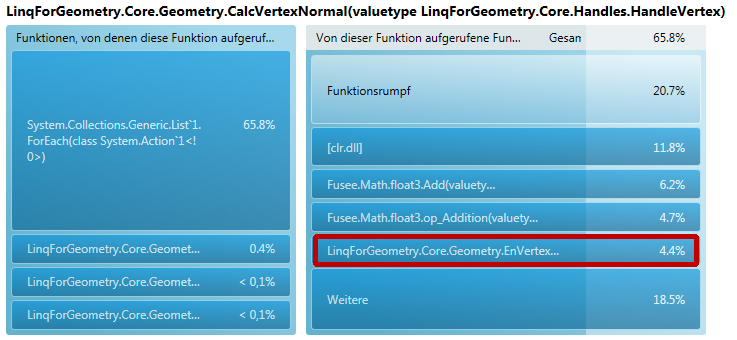
\includegraphics[width=\linewidth]{../Messung/2-linq-calcvertnormals-0}
\captionof{figure}{Messung der CalcVertexNormal() Methode}\label{messung:alg10}
\end{minipage}
Laut Profiler ist also der in der CalcVertexNormal() Methode benutze Enumerator EnVertexIncomingHalfEdge() \footnote{Beschriebener Wert blau markiert} mit 4.4\% Inklusiven Samplings in seiner Ausf"uhrung sehr sparsam. Der Algorithmus, welcher die Topologie der \HES ausnutzt um keine riesigen Datenmengen bearbeiten zu m"ussen, ist in dieser Form also sehr effizient.
\newline

Hier ist zu sehen, dass die Ausf"uhrung des Enumerators im gesamt Kontext einer Messung einen sehr kleinen Anteil sowohl an Inklusiven Samplings (4,38\%) und Exklusiven Samplings (1.74\% ) h"alt.
\begin{minipage}[c][7cm]{\linewidth}
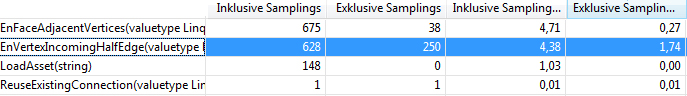
\includegraphics[width=\linewidth]{../Messung/2-linq-envertexinche-0}
\captionof{figure}{Messung des Enumerators EnVertexIncomingHalfEdge() im Gesamtkontext einer Demo Anwendung ohne LINQ. Die relevante Zeile ist blau markiert.}\label{messung:alg11}
\end{minipage}
%%%%%%%%%%%%%%%%%%%%%%%%%%%%%%%%%%%%Nativ%%%%%%%%%%%%%%%%%%%%%%%%%%%%%%%%
%%%%%%%%%%%%%%%%%%%%%%%%%%%%%%%%%%%%Methodensyntax%%%%%%%%%%%%%%%%%%%%%%%

\subsubsection{Messergebnis f"ur die Methodensyntax (alg2) aus \ref{code:alg2}}
\begin{minipage}[c][8cm]{\linewidth}
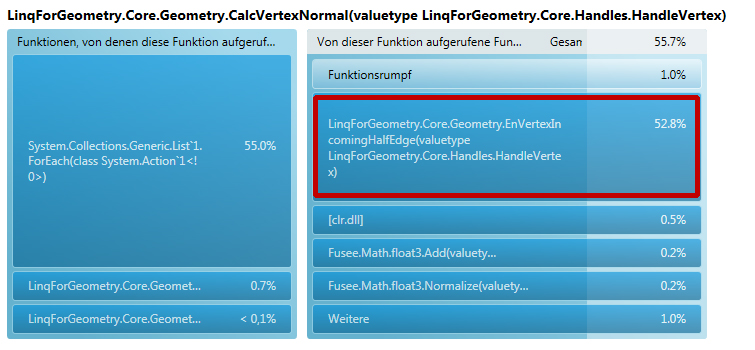
\includegraphics[width=\linewidth]{../Messung/2-linq-calcvertnormals-1}
\captionof{figure}{Messung der CalcVertexNormal() Methode.}\label{messung:alg20}
\end{minipage}
Bei dieser Variante sind die Inklusiv Samples f"ur den Enumerator mit 52.8\% sehr viel h"oher als im vorigen Vergleich \ref{messung:alg10}. Der hohe Wert ergibt sich hier durch die LINQ Abfrage innerhalb des Iterators und deren Aufrufe an das System. Zu sehen in Abbildung \ref{messung:alg210}.

\begin{minipage}[c][8.5cm]{\linewidth}
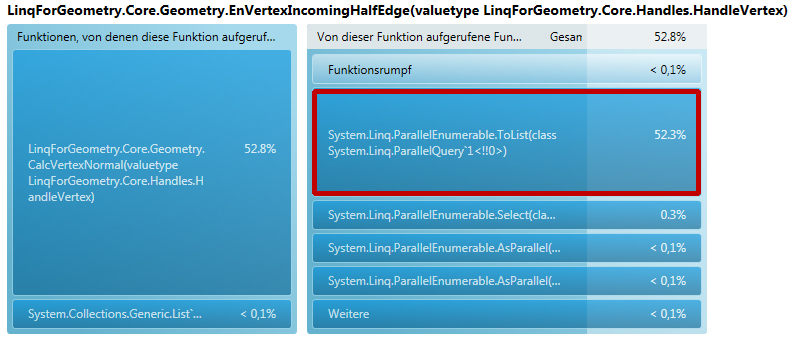
\includegraphics[width=\linewidth]{../Messung/2-linq-envertexinche-1-0}
\captionof{figure}{Messung des Enumerators EnVertexIncomingHalfEdge() in Methodensyntax.}\label{messung:alg210}
\end{minipage}
Die Inklusiven Samplings dieser Methode sind sehr gering. Dieser Zustand ergibt sich daraus, dass ausser dem LINQ Query Aufruf und dem Return Wert nichts weiter in dieser Funktion geschieht. Die gro"se Auslastung dieser Methode schl"agt sich im hohen Wert der Inklusiv Samples nieder. Zur Methode in \ref{messung:alg10} besteht ein Unterschied von 48,42\%. Die Auslastung des benutzen CPU KernsTest Systems lag mit dieser Methode nahe an 100\% und nie unter 80\%.

\begin{minipage}[c][5cm]{\linewidth}
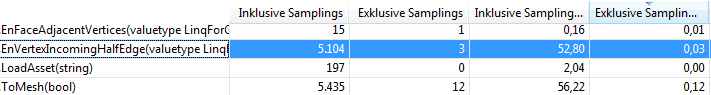
\includegraphics[width=\linewidth]{../Messung/2-linq-envertexinche-1}
\captionof{figure}{Messung des Enumerators EnVertexIncomingHalfEdge() in Methodensyntax im Kontext eines Demo Ablaufs.}\label{messung:alg21}
\end{minipage}

Die hohen Messergebnisse des Iterators resultieren aus der sehr gro"sen Collection an Half-Edges "uber welche die LINQ Abfrage iterieren muss, um alle eingehenden Half-Edges eines Vertex zu finden. Der Native Algorithmus ben"otigt hier im Gegenzug nur ein paar Pointer Spr"unge "uber Nachbar (Twin)Half-Edges wie in \ref{code:alg1} dargestellt. \label{ref:linqNativeSampling1}

%%%%%%%%%%%%%%%%%%%%%%%%%%%%%%%%%%%%Methodensyntax%%%%%%%%%%%%%%%%%%%%%%%
%%%%%%%%%%%%%%%%%%%%%%%%%%%%%%%%%%%%Abfragesyntax%%%%%%%%%%%%%%%%%%%%%%%

\subsubsection{Messergebnis f"ur die Abfragesyntax (alg3) aus \ref{code:alg3}}
\begin{minipage}[c][8cm]{\linewidth}
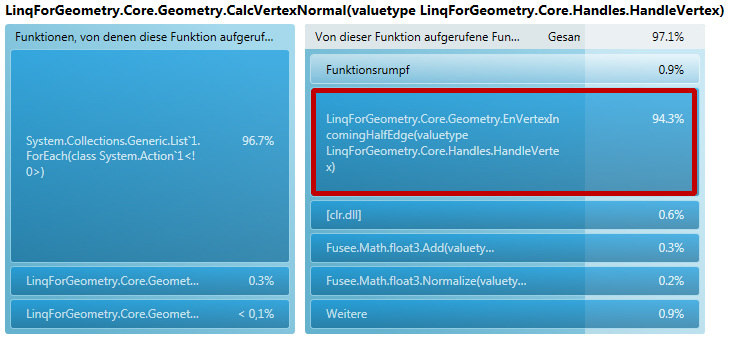
\includegraphics[width=\linewidth]{../Messung/2-linq-calcvertnormals-2}
\captionof{figure}{Messung der CalcVertexNormal() Methode.}\label{messung:alg30}
\end{minipage}

In der Abfragesyntax steigt der Wert der Inklusive Samples des Enumerators im Gegensatz zur Methodensyntax. Er liegt hier bei 94.3\%. Dieser Zustand ergibt sich wie in Abbildung \ref{messung:alg31} ersichtlich aus dem h"oheren Aufwand des ToList() Konverters. Eine weitere Parallelisierung im Enumerator durch Angabe von AsParallel(), wie in \ref{code:alg2}, kann hier wegen einer Einschr"ankung der Abfragesyntax nicht erfolgen.

\begin{minipage}[c][10cm]{\linewidth}
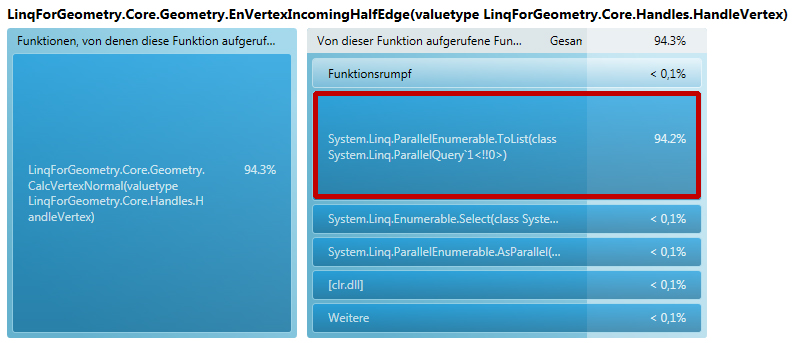
\includegraphics[width=\linewidth]{../Messung/2-linq-envertexinche-2-0}
\captionof{figure}{Messung des Enumerators EnVertexIncomingHalfEdge() in Abfragesyntax.}\label{messung:alg31}
\end{minipage}

Im Kontext einer kompletten Demo Anwendung steht der Enumerator mit 14846 Inklusiv Samples im Vergleich mit dem ersten vorgestellten Algorithmus in Abbildung \ref{messung:alg11} nicht sehr gut da.
\begin{minipage}[c][5cm]{\linewidth}
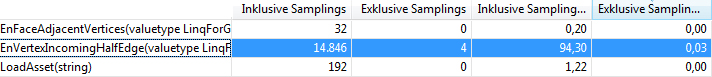
\includegraphics[width=\linewidth]{../Messung/2-linq-envertexinche-2}
\captionof{figure}{Messung des Enumerators EnVertexIncomingHalfEdge() in Abfragesyntax im Kontext eines Demo Ablaufs.}\label{messung:alg32}
\end{minipage}
%%%%%%%%%%%%%%%%%%%%%%%%%%%%%%%%%%%%Abfragesyntax%%%%%%%%%%%%%%%%%%%%%%%

\subsection{Zusammenfassung der Erkenntnisse aus den Messwerten}
Aus den genannten Werten ist also ersichtlich, dass LINQ Abfragen auf gro"sen Datenmengen in LFG nach M"oglichkeit vermieden werden sollten. Im Falle der Messwerte handelt es sich bei dem Utah Teapot um eine Liste aus 1400+ (Half-Edge) Elementen. Diese Elemente m"ussen f"ur jeden Vertice, um seine Normale zu berechnen, einmal durchsucht werden. Somit w"urde sich mit den LINQ Abfragen mindestens ein Algorithmus der Komplexit"at $n^2$ ergeben. Wann immer es m"oglich ist, sollten die Vorteile der Datenstruktur im Entwurf von Enumeratoren/Iteratoren auch benutzt werden um die Performance so gut es geht zu erhalten.
\newpage

\subsection{Benchmarking mit verschiedenen 3d Modellen}
Das folgende Diagramm \ref{diag:benchmark} beschreibt Benchmark Ergebnisse welche mit Hilfe einer Fusee Demo Anwendung\footnote{Die f"ur die Messung benutze Demo Anwendung befindet sich im Fusee Beispielprojekt von \LFG. Sie kann durch verschiedene Settings aktiviert werden. Der Quellcode dokumentiert die ben"otigten Variablen.} ermittelt wurden. Gemessen wurde die Transformation von verschiedenen beispielhaften 3d Modellen. Zu diesen Modellen z"ahlen einfachste geometrische Gebilde aber auch komplexere Modelle aus der Computergrafik und ein Modell aus dem 3D Computerspiel "`Doom 3"'. Insgesamt wurden zw"olf Messungen durchgef"uhrt. Die ermittelte Gr"o"se Frames per Second (FPS) kann hier an der x-Achse des Diagramms abgelesen werden. Alle Modelle wurden mit und ohne Vertex Normalen Berechnung gemessen. Die Fusee seitige Beleuchtung war nur im Falle der Messung mit der Vertex Normalen Berechnung aktiv. F"ur jedes Modell wurde die gleiche Textur verwendet.
\newline

Diese Messung zeigt den Einfluss der Vertex und Polygon Anzahl auf das System zur Laufzeit. Bei den komplexeren Modellen mit einer Polygonanzahl > 200 f"uhrt das Aktivieren der Vertex Normalen Berechnung zu einer reduktion der FPS auf $1/3$ der FPS der Basis Messung ohne Vertex Normalen Berechnung. Diese Tatsache zeigt, dass eine Berechnung solch gro"ser Datenmengen und der darin benutzen Iterationen einiges an Leistung kostet. Die verwendete Methode zur Berechnung der Vertex Normalen ist Kantenbasiert und kann daher nur in einer Datenstruktur wie der \HES eingesetzt werden. In einer Face basierten Datenstruktur w"are diese Berechnung nur noch weiteren erheblichen Mehraufwand zu schaffen.

%%%%%%%%%%%%%%%%%%%%%%%%%%%%%%%%%%%%Diagramm der Messungen%%%%%%%%%%%%%%%%%%%%%%%
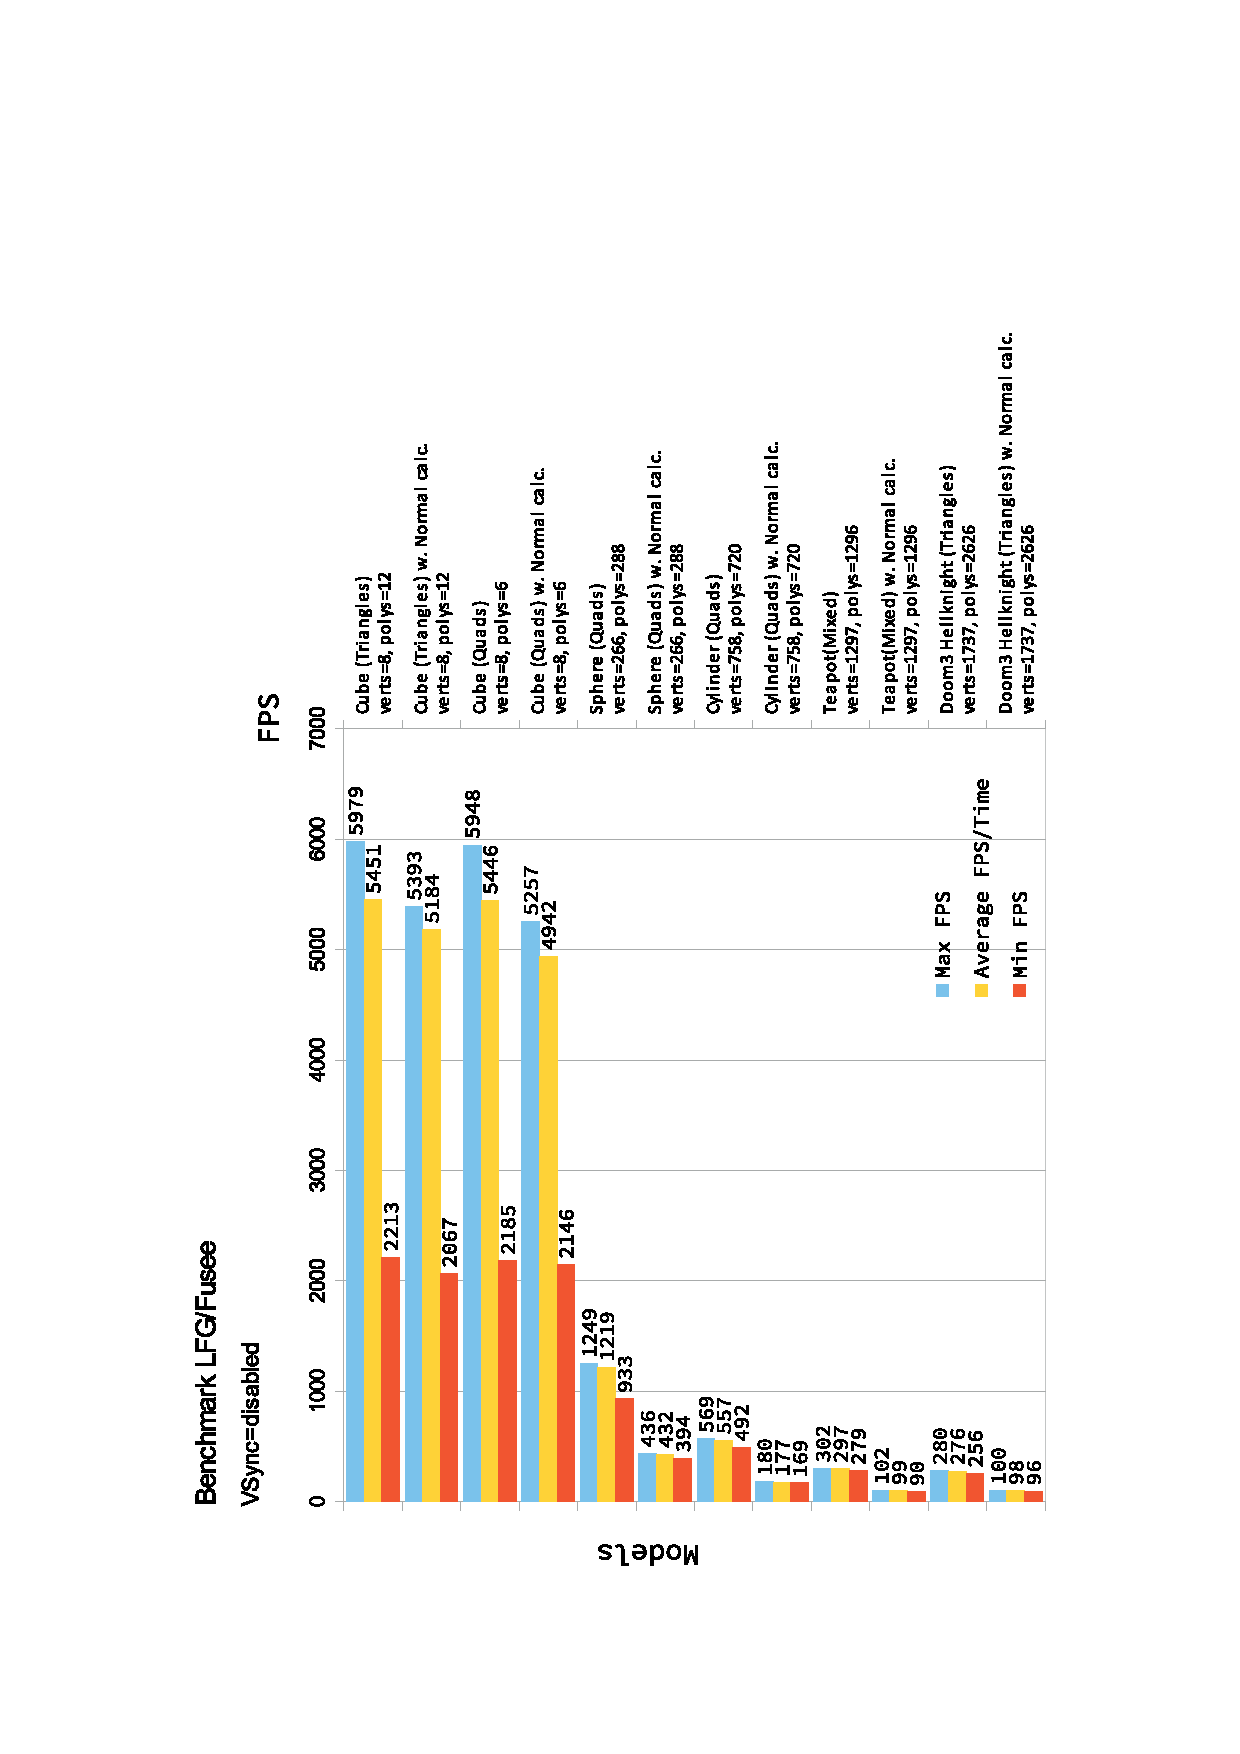
\includepdf[pages={1}, pagecommand={}]{../Messung/Benchmarks.pdf} \label{diag:benchmark}
%%%%%%%%%%%%%%%%%%%%%%%%%%%%%%%%%%%%Diagramm der Messungen%%%%%%%%%%%%%%%%%%%%%%%


			%Content
		%\subsection {Verwendete „Design-Patterns“ und Softwarelösungen}
			%Content
			%Content

	\section {Manipulation von Mesh Daten in der Datenstruktur}
		%Content
		Um die Mesh Daten eines Geometry Objektes zu manipulieren gibt es verschiedene M"oglichkeiten. Durch Manipulationen kann das Mesh geringf"ugig oder gar komplett ver"andert werden. Es ist allerdings wichtig, keine Verbindungen der Datenstruktur im Geometry Objekt zu besch"adigen. Ein Geometry Objekt h"alt zwei verschiedene Arten von Daten vor. Zum einen sind dies "`reale Daten"'. Dabei handelt es sich um tats"achliche Werte, also in etwa Vertex Koordinaten, Vertex Normalen, Face Normalen und UV Koordinaten. Zum anderen existieren virtuelle Beziehungen der einzelnen Elemente der Datenstruktur untereinander, die hier als Half-Edges, Edges, Vertices und Faces bezeichnet werden. Um also die Form eines Meshes zu ver"andern m"ussen also in aller Regel die Beziehungen der Elemente ver"andert werden. Ein einfaches Beispiel dazu w"are die Triangulation eines Meshs. Es werden hierbei keine neuen realen Daten erzeugt sondern lediglich Half-Edges, Edges und Faces manipuliert.
\newline

Beide Manipulationsarten k"onnen aber auch kombiniert werden. Ein klassischer Fall w"are ein Subdivision Surfacing Algorithmus welcher durch Erweiterung des Geometry Objektes das Mesh in seiner Form ver"andern w"urde. Hierbei ver"andern sich alle Teile eines Geometry Objektes. Es entstehen neue Kanten und Faces und es werden neue Vertices aus bereits vorhandenen berechnet und eingef"ugt. 
		%Content
		\subsection {Manipulation von Edges und Half-Edges}
			%Content
			Half-Edges sind das wichtigste Konstrukt in der Datenstruktur. Daher sind sie auch der interessanteste Ansatz zur Manipulation von Meshes. Die Triangulation eines Quadrilateral Meshes in \LFGS ist ein gutes Beispiel f"ur eine einschl"agige Ver"anderung des Mesh Objekts durch Manipulation und Einf"ugen neuer Half-Edges. Durch wenige "Anderungen an den Pointern der vorhandenen Half-Edges und das einf"ugen von zweier neuer Half-Edges kann ein Quad trianguliert werden.

			%Content
		\subsection {Manipulation von Vertices}
			%Content
			Vertices k"onnen in \LFGS durch Ver"anderung ihrer Half-Edge Pointer oder durch direkte "Anderung ihrer tats"achlichen Werte manipuliert werden. Diese Tatsache wird von \LFGS im Algorithmus f"ur die Mesh Skalierung eingesetzt. Durch Matrixmultiplikation jedes Vertex mit der gleichen Skalierungsmatrix kann das Objekt entlang aller drei Achsen (X, Y, Z) gleichzeitig oder getrennt skaliert werden. Um z.B. eine Translation zu erreichen werden alle Vertices mit einer anderen Matrix multipliziert. Das gleiche gilt f"ur eine Rotation. Vertex Manipulation ist also unersetzlich f"ur die Ver"anderung der Daten im dreidimensionalen Raum.
			%Content
		\subsection {Manipulation von Faces}
			%Content
			Faces bieten am wenigsten Manipulationsm"oglichkeiten in \LFG. Nur der Index auf die Normale und der Pointer auf eine begrenzenden Half-Edge des Face kann ver"andert werden. Faces besitzen keine physischen Daten (bis auf die Face Normale). Sie sind darum aber nicht weniger wichtig. Denn viele Manipulationsalgorithmen wie die Triangulation eines Meshes oder die Vertex Normalen Berechnung befassen sich mit den Faces als Einstiegspunkt in die geometrische Operation.
			%Content
	\section {Beispielhafte Implementierung von Standard Algorithmen zur Geometriemanipulation als Modul}
			%Content
	\LFGS bietet zur beispielhaften Manipulation eines Geometry Objekts verschiedene Methoden an. Alle diese Methoden sind im Modul Projekt LinqForGeometry.ExternalModules in der Static Klasse Transformations zu finden.

Zu ihnen z"ahlen:
\begin{itemize}
\item Die Transformation des Objekts durch die "Ubergabe von Faktoren pro Achse.
\item Die Skalierung durch die Angabe von Faktoren pro Achse.
\item Eine Translation durch Übergabe von Faktoren pro Achse.
\item Eine Rotation um die Globale X, Y oder Z Achse.
\end{itemize}

\subsection {Transformation mit einer Transformationsmatrix}
%Content
Um die Vertices eines Meshes zu transformieren wird eine zuvor in der Methode zusammengestellte Transformationsmatrix auf jeden Vertex des Meshes angewendet. Ohne LINQ w"urde man in einer Schleife "uber jeden Vertex laufen und das Ergebnis wieder in eine neue Liste schreiben "mussen. Diese Liste m"usste dann die aktuelle Vertex Liste im Mesh "uberschreiben um die neuen Werte zu "ubernehmen.

Durch die Nutzung von LINQ entwickelt sich der oben genannte Algorithmus zu einem Einzeiler und zeigt hier sehr gut warum LINQ die Entwicklung solcher Algorithmen sehr viel lesbarer und einfacher gestaltet. Die hier gezeigte LINQ Abfrage ist in der Methodensyntax geschrieben.
\lstinputlisting
			[caption={Transformation.cs - Manipulation der Vertices}, label=code:transform, firstline=95, lastline=108]
			{../../HFU_Fusee/Fusee/src/Engine/LinqForGeometry/LinqForGeometry.ExternalModules/Transformations/Transformations.cs}

Das Geometry Objekt wird dieser Methode lediglich Call by Reference "ubergeben um die ben"otigte Rechenleistung zu minimieren und die Bearbeitung mit der einzeiligen LINQ Funktion m"oglich zu machen. So werden die Daten direkt ohne zwischenspeichern ressourcenschonend auf der Quelle ver"andert, ohne dass das Ergebnisset dann nochmal explizit gespeichert oder "ubergeben werden muss.
			%Content
\newpage
	\section {Berechnungen f"ur die Darstellung eines Meshes in der Fusee Engine}
	%Content
	Um ein in der \LFGS \HES gespeichertes Mesh in der Fusee Engine zu rendern bedarf es einiger Operationen. Die wichtigsten Operationen f"ur die Vorbereitung der Darstellung sind alle in der LFG Methode ToMesh() zu finden. Diese Methode kann als Konverter bezeichnet werden. Um LFG an eine andere Engine anzupassen m"usste diese Operation falls n"otig ge"andert werden. ToMesh() pr"uft zuerst ob der Benutzer eine Triangulation des Meshes w"unscht. Falls ja wird das Mesh beim ersten Rendern nach ToMesh trianguliert. Diese "Anderung ist zur Laufzeit nicht R"uckg"angig zu machen. Es folgen jetzt einige Schritte die f"ur eine sp"atere Beleuchtungsberechnung in Fusee n"otig sind.

Die Face Normalen werden jetzt durch CalcFaceNormal(HandleFace face) berechnet. Diese Methode sucht alle Vertices eines Faces heraus und berechnet aus den ersten drei Vertices des Faces durch das Kreuzprodukt eine Normale f"ur das aktuelle Face. Diese Normale wird jetzt in eine Liste eingetragen und ein Handle auf sie wird am Face gespeichert. Die Face Normalen sind ein wichtiges Element um im n"achsten Schritt die Vertex Normalen berechnen zu k"onnen welche in Fusee f"ur eine korrekte Beleuchtung des Modells verantwortlich sind.

Vertex Normalen f"ur Fusee werden in \LFGS durch die Methode CalcVertexNormal(HandleVertex vertex) berechnet. Diese Berechnung ist eine der aufw"andigsten Kalkulationen im Projekt. F"ur jede Eingehende Half-Edge auf einen Vertex wird eine Vertex Normale berechnet. Daraus ergibt sich, dass jedes Face beim Konvertieren nach Fusee.Mesh f"ur den Vertex jeden Vertex eine Normale erh"alt um Kanten und Abstufungen korrekt auszuleuchten. Die Methode gliedert sich wie folgt:

\begin{itemize}
\item Es werden alle eingehenden Half-Edges eines Vertex gesucht.
\item F"ur jede Half-Edge gilt Folgendes:
	\begin{itemize}
	\item Pr"ufe ob die Half-Edge zu einem Face geh"ort um keine L"ocher im Mesh anzusprechen und dadurch Nullpointer zu provozieren.
	\item Frage die Normale des zur Half-Edge geh"orenden Faces ab.
	\item Lege eine Ergebnisvariable an welche sp"ater alle n"otigen aufsummierten Normalen enth"alt.
		\begin{itemize}
		\item Iteriere "uber jede andere eingehende Half-Edge.
		\item Entspricht diese Half-Edge jener f"ur welche gerade die Normale berechnet wird, so addiere einmal ihre Normale zum Ergebnis.
		\item Ist es eine andere Half-Edge, dann vergleiche den Winkel zwischen beiden Face Normalen und addiere die Half-Edge nur wenn der Winkel kleiner als der in \_constSmoothingAngle gew"ahlte Threshold ist.
		\end{itemize}
	\item Sind alle n"otigen Normalen addiert muss der erhaltene Ergebniswert an der Half-Edge gespeichert und der Algorithmus bearbeitet die n"achste Half-Edge im gesamt Set.
	\end{itemize}
\end{itemize}

Diese Berechnung der Vertex Normalen kann durch Setzen der Boolean Variable \_VertexNormalActive in Geometry ein oder ausgeschaltet werden. Diese Funktion wurde zu Test Zwecken w"ahrend dieser Arbeit implementiert und kann zum Debugging benutzt werden.
\newline

Sind jetzt alle Normalen berechnet, iteriert ToMesh() noch einmal "uber alle Faces und Half-Edges und sammelt die relevanten Informationen in Collections, die f"ur Fusee sp"ater in Arrays konvertiert werden. Hierbei werden, da Fusee aktuell nur mit Triangles arbeitet (Stand Juli 2013), auch die Triangles neu berechnet. Dazu "lauft ein Iterator "uber die Half-Edges des Meshes und speichert die Indizes der Vertices in der richtigen Reihenfolge in einer Liste ab.

Die meisten OpenGL Echtzeit 3D Engines benutzen aktuell nur noch Triangles f"ur die repr"asentation der Meshes. OpenGL hat die Funktion GL\_QUADS in OpenGL 3.1 und dar"uber entfernt und in 3.0 gilt diese Funktion als "deprecated".
\begin{quote}"`GL\_QUADS [...] have been removed from core OpenGL 3.1 and above (they are only deprecated in OpenGL 3.0).\footnote{\url{http://www.opengl.org/wiki/Primitive} (gepr"uft 30.07.2013 Abschnitt "`Quads"')}
"'\end{quote}

Man hat sich f"ur Triangles entschieden, da sie zur Repr"asentation von Meshes sehr gut geeignet sind. Ein Quad besteht genauer gesagt nur aus zwei Triangles und deswegen sollte die OpenGL API nicht mit zus"atzlichen Konvertierungen belastet werden. Die Khronos Group, welche f"ur die Entwicklung und Wartung von OpenGL zust"andig ist beschrieb im M"arz 2009 in der Spezifikation zu OpenGL 3.1, dass die OpenGL API in Zukunft "`ausged"unnt"' oder "`schlanker"' gemacht werden soll.\footnote{\url{https://www.khronos.org/news/press/khronos-releases-streamlined-opengl-3.1-specification}}
\newpage
\begin{quote}"`Many algorithms use triangle meshes for representing geometric surfaces. The simple triangle can serve as a basic surface primitive to adaptively approximate smooth freeform geometry. A triangle mesh naturally allows to adapt the required number of primitives to the geometric shape instead of the basic topology of an arbitrary object. Triangle meshes are efficient, since the triangle is currently the only surface patch that is directly supported by computer graphics hardware and even software rendering methods like ray tracing or radiosity prefer to use piecewise linear primitives to represent geometric objects due to gains in performance."' \cite[S.~1]{Campagna.1998}\end{quote}

Um die Konvertierung in ein Fusee Mesh Objekt abzuschliessen, muss die ToMesh() Methode ein Objekt von dem Fusee bekannten Datentypen "`Fusee.Mesh"' erzeugen und es an den Aufrufer, in Fall dieses Projektes dem Fusee Beispiel Projekt "`LinqForGeometry"', zur"uckgeben. Das so erzeugte Objekt kann dann in der eigenen Fusee App oder eben dem Beispielprojekt mit einem Aufruf auf die im RenderContext enthaltene Methode "`Render()"', RC.Render(Mesh meshObjekt), angezeigt werden.

	%Content
	%\section {Implementierung von Catmull Clark als Modul f"ur \LFG}
			%Content
			%Content
	%	\subsection {Was ist der Catmull Clark Algorithmus?}
				%Content
				%Content
	%	\subsection {Vorteile der Implementierung in der HES}
				%Content
				%Content

%\section {Welche M"oglichkeiten zur Erweiterung durch eigenen Code bietet \LFG}
				%Content
				% Module, zb das Transformationsmodul. Zusätzlich schauen ob man sagen kann das Catmull Clark als Modul läuft etc.

%%%%%%
%	Hauptteil ENDE
%%%%%%



%%%%%%
%	Schluss START
%%%%%%

\chapter {Schluss}
	\section {Fazit}
		%Content
		Zum Ende dieser Arbeit hat sich \LFGS von einer simplen Datenstruktur in eine in die Fusee Engine integrierte Umgebung zum Handling und zur Manipulation von 3D Meshes entwickelt. Das Projekt hat einen Zustand erreicht, in welchem es m"oglich ist, Meshes zu laden, sie anzuzeigen und verschiedene Elemente des Meshes gezielt zur Laufzeit zu ver"andern. Texturen und Vertex Normalen Beleuchtungsberechnung werden in der Datenstruktur durch die Integration in Fusee unterst"utzt. Das Projekt kann um eigenen Code erweitert werden und bietet eine grundlegende Auswahl an Enumeratoren/Iteratoren f"ur sp"atere Entwicklungen. Es w"are interessant mit diesem Projekt einen 3D Echtzeit Editor in der Fusee Engine zu implementieren. LINQ Abfragen k"onnen nach Wunsch verwendet werden um eigene Enumeratoren/Iteratoren zu entwicklen oder bestehende zu kombinieren. Einige LINQ Abfragen werden f"ur Transformationen auf den Meshes genutzt. Hierzu werden Transformationsmatrizen mit Vertices multipliziert.

Trotz der vielen M"oglichkeiten in Iteratoren und Transformationen muss bei der Verwendung der \HES in Verbindung mit LINQ auf die Gr"o"se der Quelldatens"atze in Relation mit dem erwarteten Ergebnisset geachtet werden. Auch hier gelten die allgemeinen Regeln zur Entwicklung von Algorithmen. "Uber eine gro"se Liste mit hunderten von Datens"atzen zu iterieren um einen oder wenige Werte abzurufen l"asst sich auch durch LINQ kaum performant gestalten. Vor allem bei zeitkritischen Operationen kann dies ein Problem darstellen. Algorithmen sollten in einem solchen Fall die Topologie der Datenstruktur nutzen.

Die gr"ossten St"arken zeigen LINQ und Lambda dann, wenn relativ kleine oder bereits gefilterte Ergebnis Datens"atze bearbeitet, weiter gefiltert oder auf andere Datentypen gemapped werden m"ussen. Diese LINQ Statements sind oft als sehr effektive Einzeiler zu schreiben und leicht zu verstehen und zu ver"andern. Im Projekt wurden also komplexe, zeitkritische Algorithmen als "`native"' Operationen direkt auf der Topologie Datenstruktur entworfen. Es hat sich gezeigt, dass aus wenigen dieser Algorithmen, eine ganze Reihe an grundlegenden LINQ basierten Iteratoren kombiniert werden konnte. Die Basis f"ur f"unf der sieben bereit gestellten Iteratoren bilden die zwei wichtigsten Iteratoren des Programms, welche wiederum als direkte Operationen auf der Datenstruktur entworfen wurden.

%!TODO! Erweiterung für Code? internal und so ...

Der Support f"ur LINQ und Lambda in einer Echtzeit 3D Datenstruktur ist also durchaus m"oglich. Er unterliegt durch die genannten Punkte einigen wenigen Einschr"ankungen, ist aber sicherlich als n"utzliche Erweiterung der Datenstruktur und dem gesamten \LFGS System als Datenstruktur zur Bearbeitung von Meshes zu verstehen.
		%Content
\section{Ausblick auf die zuk"unftige Verwendung von \LFG}
\LFGS ist an sich nur eine Basis f"ur weitere Entwicklungen. Das System kann an manchen Stellen noch optimiert werden. Den Anspruch an eine vollst"andig integrierte Version einer Echtzeit 3D Datenstruktur hatte \LFGS ohnehin nie. In Zukunft ist es angedacht, das Projekt m"oglicherweise als Datenstruktur f"ur einen Fusee internen 3D Echtzeit Mesh Editor zu verwenden und weitere Algorithmen zur Geometriemanipulation zu formulieren. Das System kann aber auch auf andere 3D Editoren oder Viewer angepasst werden und darf selbstverst"andlich unter Beachtung der bestehenden Lizenzen in diese integriert werden. So ist also zu hoffen, dass diese Arbeit einen Grundstein f"ur weitere interessante Projekte, nicht zuletzt in der Echtzeit 3D Engine Fusee von Herrn Prof. M"uller und seinem Team der Hochschule Furtwangen, legen konnte.

\newpage
\section {Wo ist der Code und die Dokumentation zu \LFGS zu beziehen und einzusehen?}
	%Content
	Sollte am Code von \LFGS Interesse bestehen, ist dieser f"ur alle Interessenten, auch hochschulextern, unter den folgenden GitHub Links abzurufen.
\begin{itemize}
\item Im Branch feat\_dsteffen\_LFG unter \url{https://github.com/FUSEEProjectTeam/Fusee} (gepr"uft 01.08.2013)
\item Oder im LFG eigenen GitHub Repository ohne Fusee Integration. Hier ist der Code allerdings nicht ohne Anpassungen in den Methoden zur Meshkonvertierung lauff"ahig. \url{https://github.com/DomS23/LinqForGeometry} (gepr"uft 01.08.2013)
\end{itemize}

Der gesamte Code dieser Arbeit ist "`Open Source"' und steht unter der MIT Lizenz, abrufbar auf der Webseite der "'Open Source Initative"` unter \url{http://opensource.org/licenses/MIT} (geprueft: 07.08.2013). Weitere Lizenz Informationen zum Code finden sich in der MIT-License.txt im Root Verzeichnis des Softwareprojekts.
			% Spielraum für Verbesserungen, Beleuchtung, Konvertierung in Fusee Mesh, Kanten mit mehr als 2 Faces möglich aber nicht schön, etc.

%%%%%%
%	Schluss ENDE
%%%%%%


%%%%%%%%%%%%%%%%%%%%%%%%%%%%%%%%%%%%%%%%%%%%%%%%%%%%%%%%%%%%%%%%%%%%%%%%%%%%%%%%
% Inhalt ENDE
%%%%%%%%%%%%%%%%%%%%%%%%%%%%%%%%%%%%%%%%%%%%%%%%%%%%%%%%%%%%%%%%%%%%%%%%%%%%%%%%
\part*{Appendix}


%%%%%%%%%%%%%%%%%%%%%%%%%%%%%%%%%%%%%%%%%%%%%%%%%%%%%%%%%%%%%%%%%%%%%%%%%%%%%%%%
% Source Code Verzeichnis START
%%%%%%%%%%%%%%%%%%%%%%%%%%%%%%%%%%%%%%%%%%%%%%%%%%%%%%%%%%%%%%%%%%%%%%%%%%%%%%%%
\lstlistoflistings
%%%%%%%%%%%%%%%%%%%%%%%%%%%%%%%%%%%%%%%%%%%%%%%%%%%%%%%%%%%%%%%%%%%%%%%%%%%%%%%%
% Source Code Verzeichnis ENDE
%%%%%%%%%%%%%%%%%%%%%%%%%%%%%%%%%%%%%%%%%%%%%%%%%%%%%%%%%%%%%%%%%%%%%%%%%%%%%%%%

%%%%%%%%%%%%%%%%%%%%%%%%%%%%%%%%%%%%%%%%%%%%%%%%%%%%%%%%%%%%%%%%%%%%%%%%%%%%%%%%
% Tabellen Verzeichnis START
%%%%%%%%%%%%%%%%%%%%%%%%%%%%%%%%%%%%%%%%%%%%%%%%%%%%%%%%%%%%%%%%%%%%%%%%%%%%%%%%
\listoftables
%%%%%%%%%%%%%%%%%%%%%%%%%%%%%%%%%%%%%%%%%%%%%%%%%%%%%%%%%%%%%%%%%%%%%%%%%%%%%%%%
% Tabellen Verzeichnis ENDE
%%%%%%%%%%%%%%%%%%%%%%%%%%%%%%%%%%%%%%%%%%%%%%%%%%%%%%%%%%%%%%%%%%%%%%%%%%%%%%%%

%%%%%%%%%%%%%%%%%%%%%%%%%%%%%%%%%%%%%%%%%%%%%%%%%%%%%%%%%%%%%%%%%%%%%%%%%%%%%%%%
% Abbildungsverzeichnis START
%%%%%%%%%%%%%%%%%%%%%%%%%%%%%%%%%%%%%%%%%%%%%%%%%%%%%%%%%%%%%%%%%%%%%%%%%%%%%%%%
\listoffigures
%%%%%%%%%%%%%%%%%%%%%%%%%%%%%%%%%%%%%%%%%%%%%%%%%%%%%%%%%%%%%%%%%%%%%%%%%%%%%%%%
% Abbildungsverzeichnis ENDE
%%%%%%%%%%%%%%%%%%%%%%%%%%%%%%%%%%%%%%%%%%%%%%%%%%%%%%%%%%%%%%%%%%%%%%%%%%%%%%%%

%%%%%%%%%%%%%%%%%%%%%%%%%%%%%%%%%%%%%%%%%%%%%%%%%%%%%%%%%%%%%%%%%%%%%%%%%%%%%%%%
% Bilbiographie START
%%%%%%%%%%%%%%%%%%%%%%%%%%%%%%%%%%%%%%%%%%%%%%%%%%%%%%%%%%%%%%%%%%%%%%%%%%%%%%%%
\nocite{*}
\bibliography{Citavi}
\addcontentsline{toc}{chapter}{Literaturverzeichnis}
\newpage
%%%%%%%%%%%%%%%%%%%%%%%%%%%%%%%%%%%%%%%%%%%%%%%%%%%%%%%%%%%%%%%%%%%%%%%%%%%%%%%%
% Bilbiographie ENDE
%%%%%%%%%%%%%%%%%%%%%%%%%%%%%%%%%%%%%%%%%%%%%%%%%%%%%%%%%%%%%%%%%%%%%%%%%%%%%%%%

%%%%%%%%%%%%%%%%%%%%%%%%%%%%%%%%%%%%%%%%%%%%%%%%%%%%%%%%%%%%%%%%%%%%%%%%%%%%%%%%
% UML START
%%%%%%%%%%%%%%%%%%%%%%%%%%%%%%%%%%%%%%%%%%%%%%%%%%%%%%%%%%%%%%%%%%%%%%%%%%%%%%%%
\chapter{UML Diagramme}
\subsection {UML Diagramme zur Implementierung von \LFG}
				%Content
				%TODO Ablaufdiagramm!
Die hier angeh"angten UML Diagramme wurden w"ahrend dieser Arbeit entwickelt und stellen die Basis der Implementierung dar. Diese Diagramme wurden vor der tatsächlichen Entwicklung der betreffenden Funktionen geschrieben und können kleine Unterschiede zum tatsächlichen Code aufweisen.

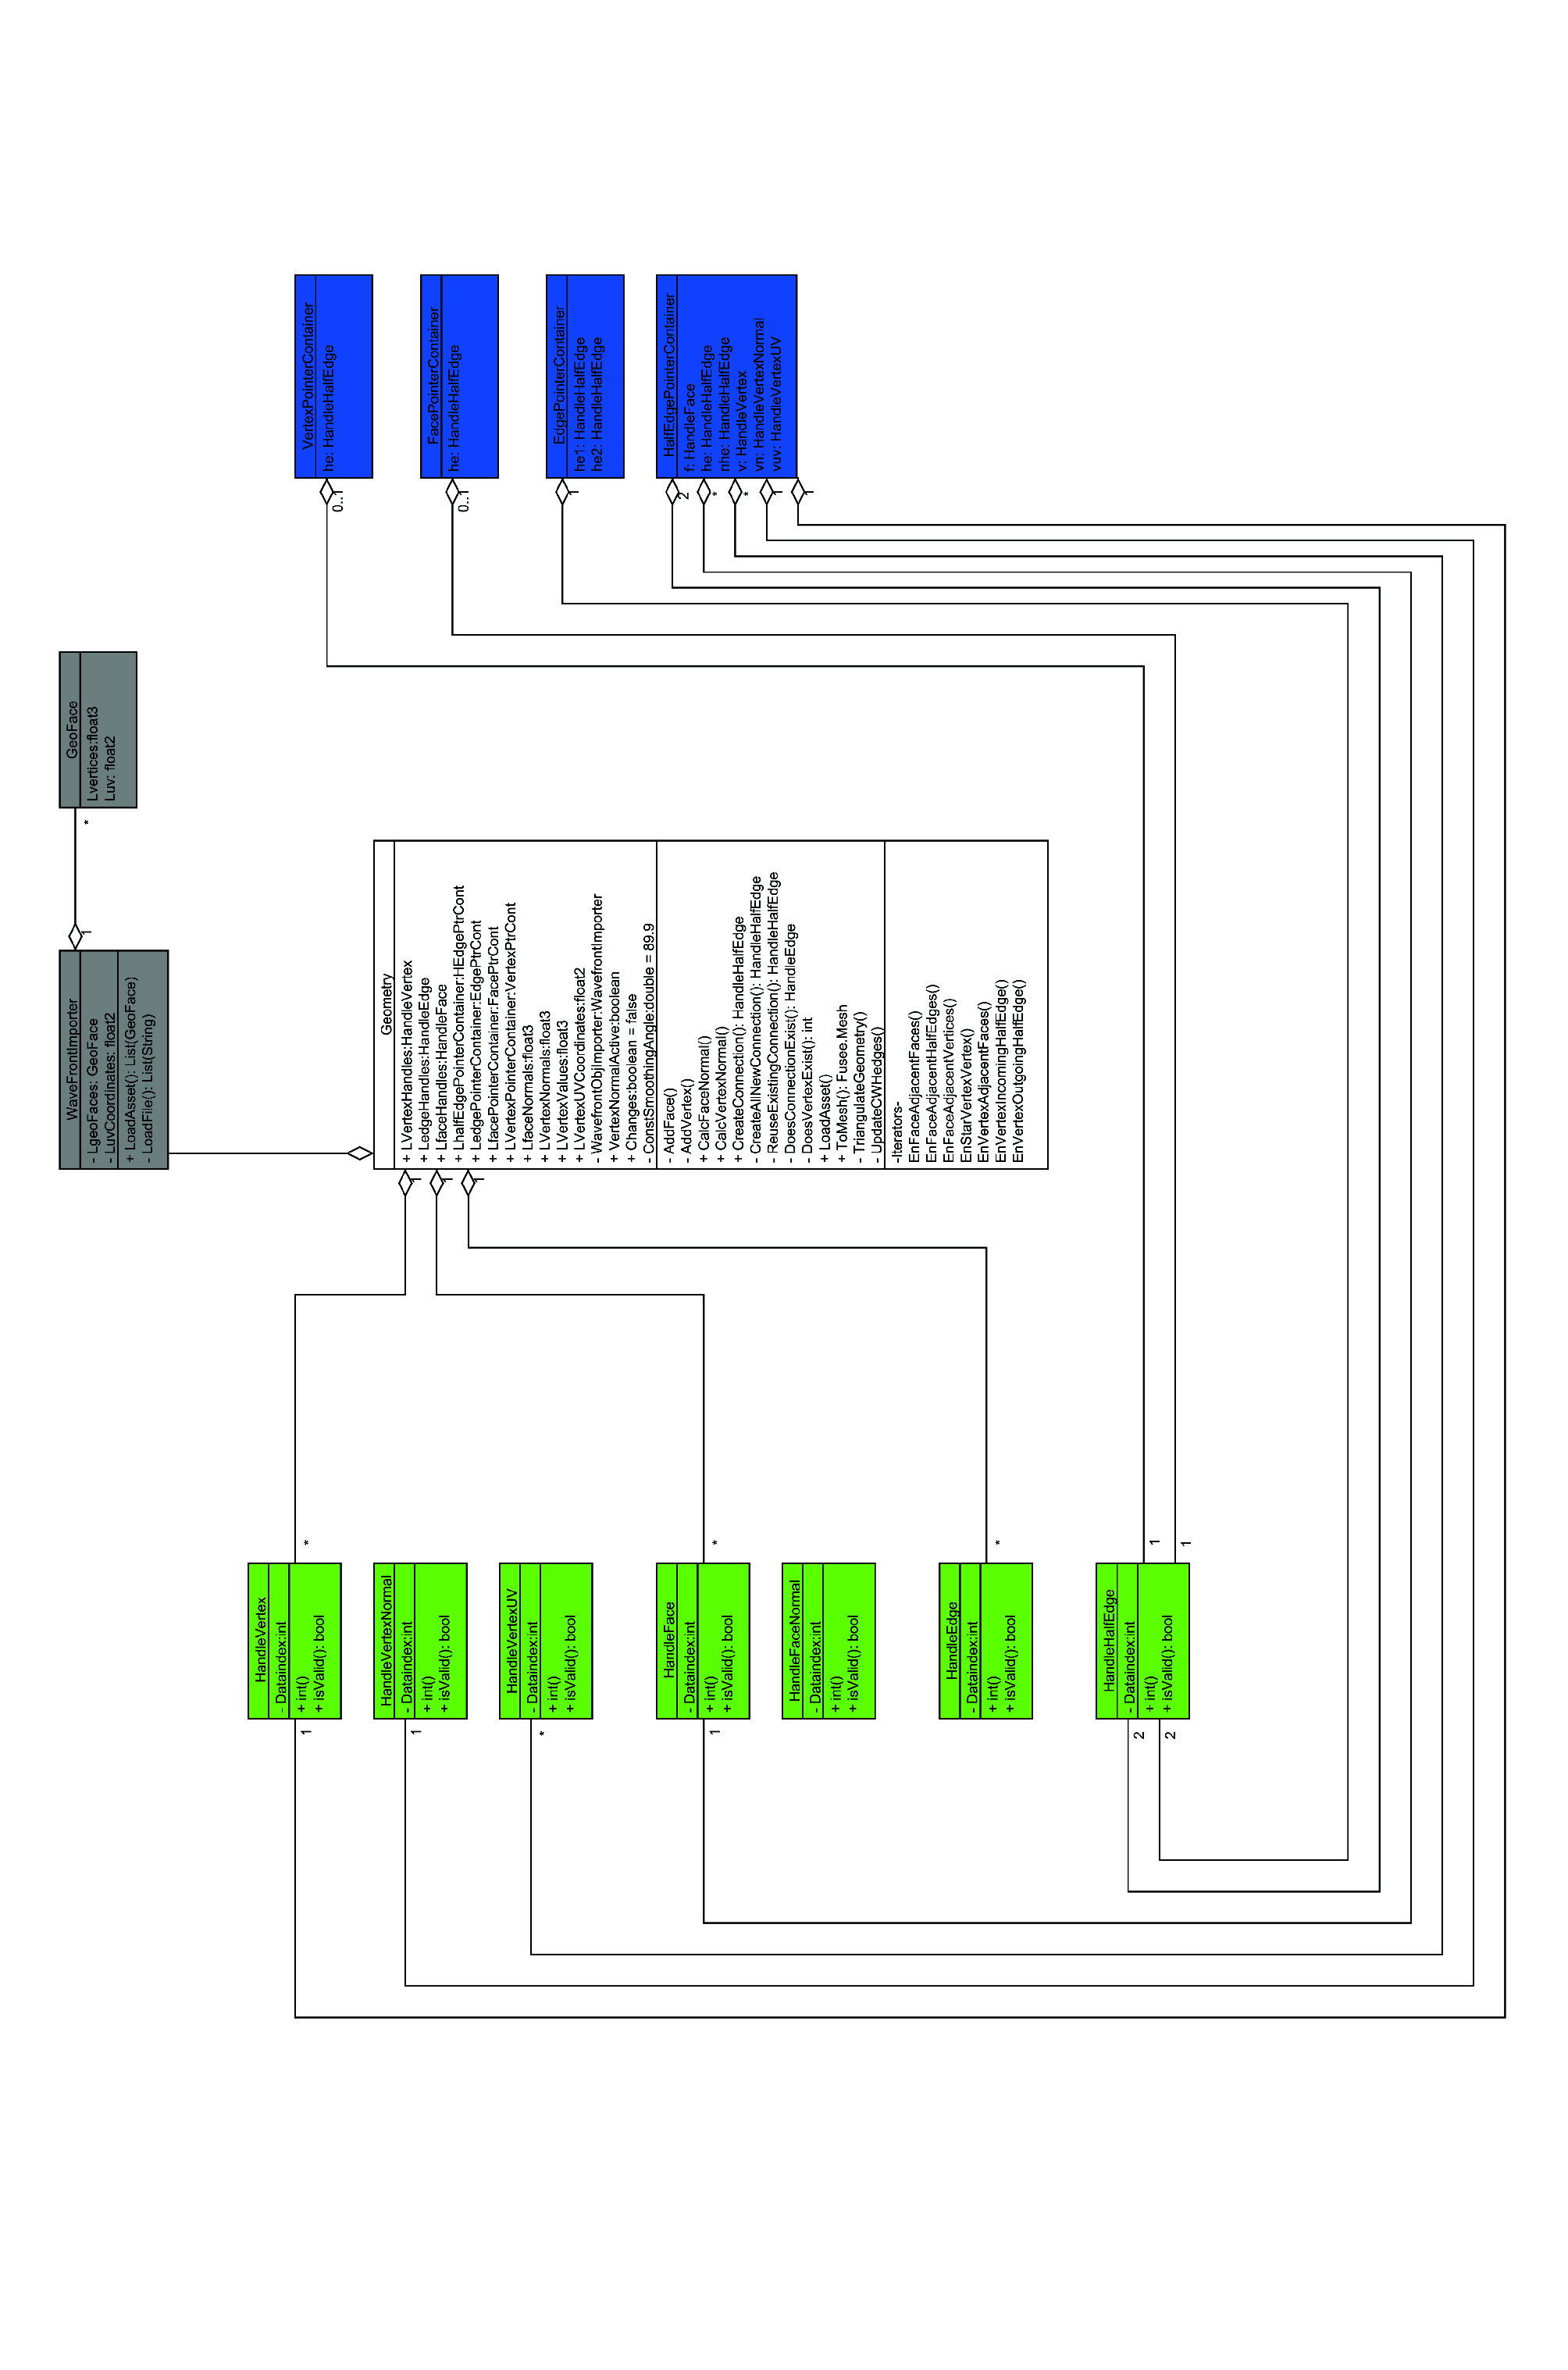
\includegraphics[width=\linewidth]{../UML/Klassendiagramm}
%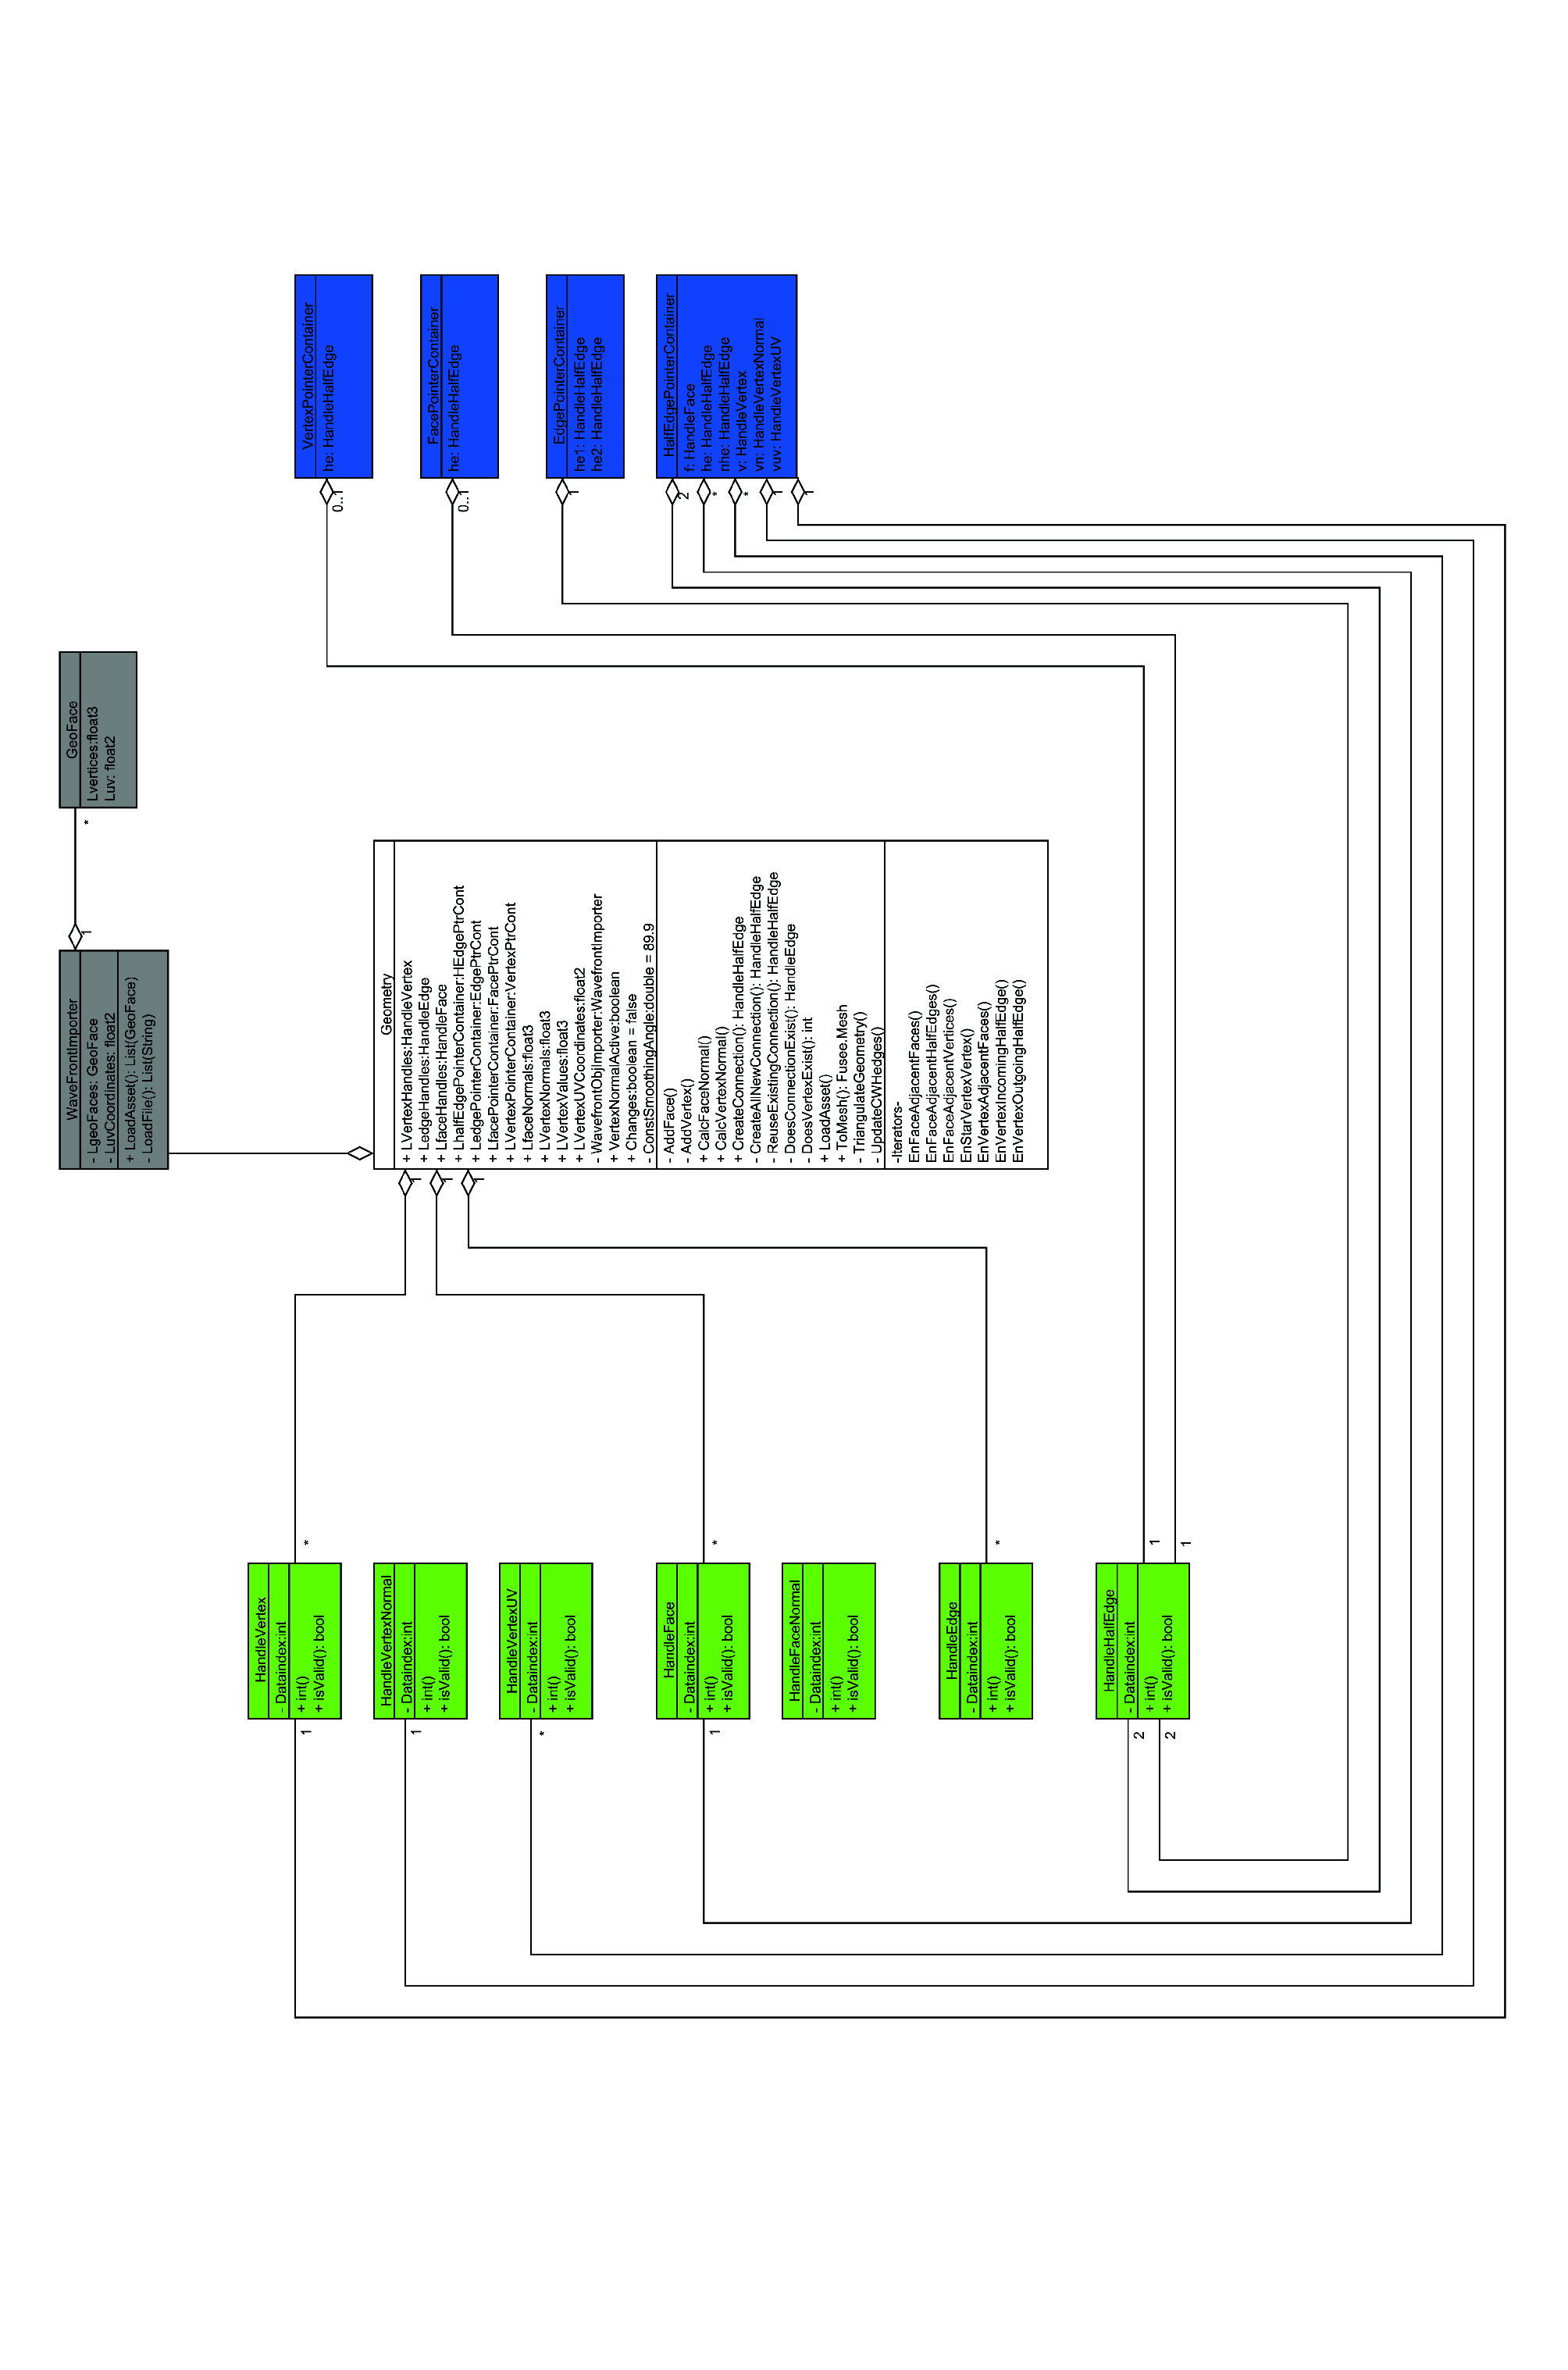
\includepdf[pages={1}, pagecommand={}]{../UML/Klassendiagramm}
\captionof{figure}{Klassendiagramm: Dieses UML Diagramm beschreibt die Implementierung des Projektes.}\label{uml:klassendiagramm}
\newpage
%\includepdf[pages={1}, pagecommand={}]{../UML/Activity-VertexIncHE}
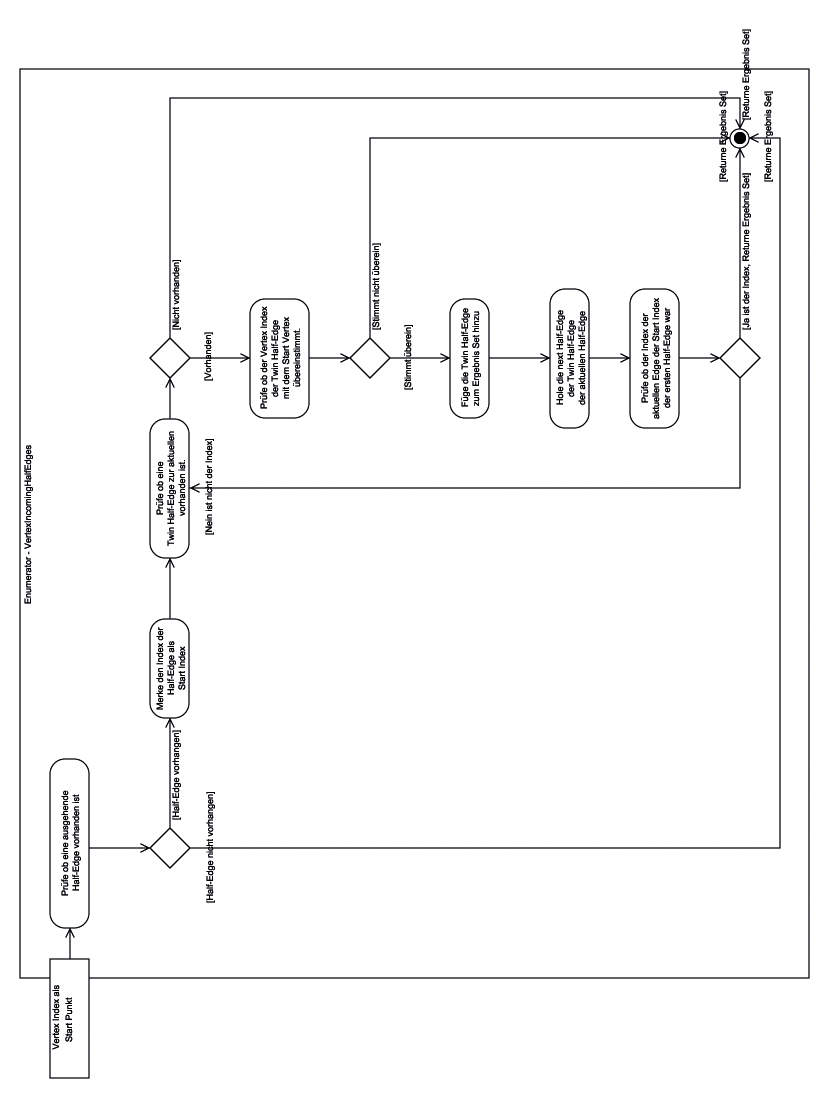
\includegraphics[width=\linewidth]{../UML/act-VertexIncHE}
\captionof{figure}{Aktivit"atsdiagramm: Der Iterator zum Finden von eingehenden Half-Edges an einem Vertex.}\label{uml:vertinche}
\newpage
%\includepdf[pages={1}, pagecommand={}]{../UML/Activity-CalcVertexNormals}
\includegraphics[width=\linewidth]{../UML/act-CalcVertexNormals}
\captionof{figure}{Aktivit"atsdiagramm: Die Methode zum Berechnen von Vertex Normalen}\label{uml:vertnc}
%%%%%%%%%%%%%%%%%%%%%%%%%%%%%%%%%%%%%%%%%%%%%%%%%%%%%%%%%%%%%%%%%%%%%%%%%%%%%%%%
% UML ENDE
%%%%%%%%%%%%%%%%%%%%%%%%%%%%%%%%%%%%%%%%%%%%%%%%%%%%%%%%%%%%%%%%%%%%%%%%%%%%%%%%

\end{document}